
\section{Benchmark CG}
\subsection{Wyniki benchmarków - platforma ARM64}

\begin{figure}[H]
    \centering
    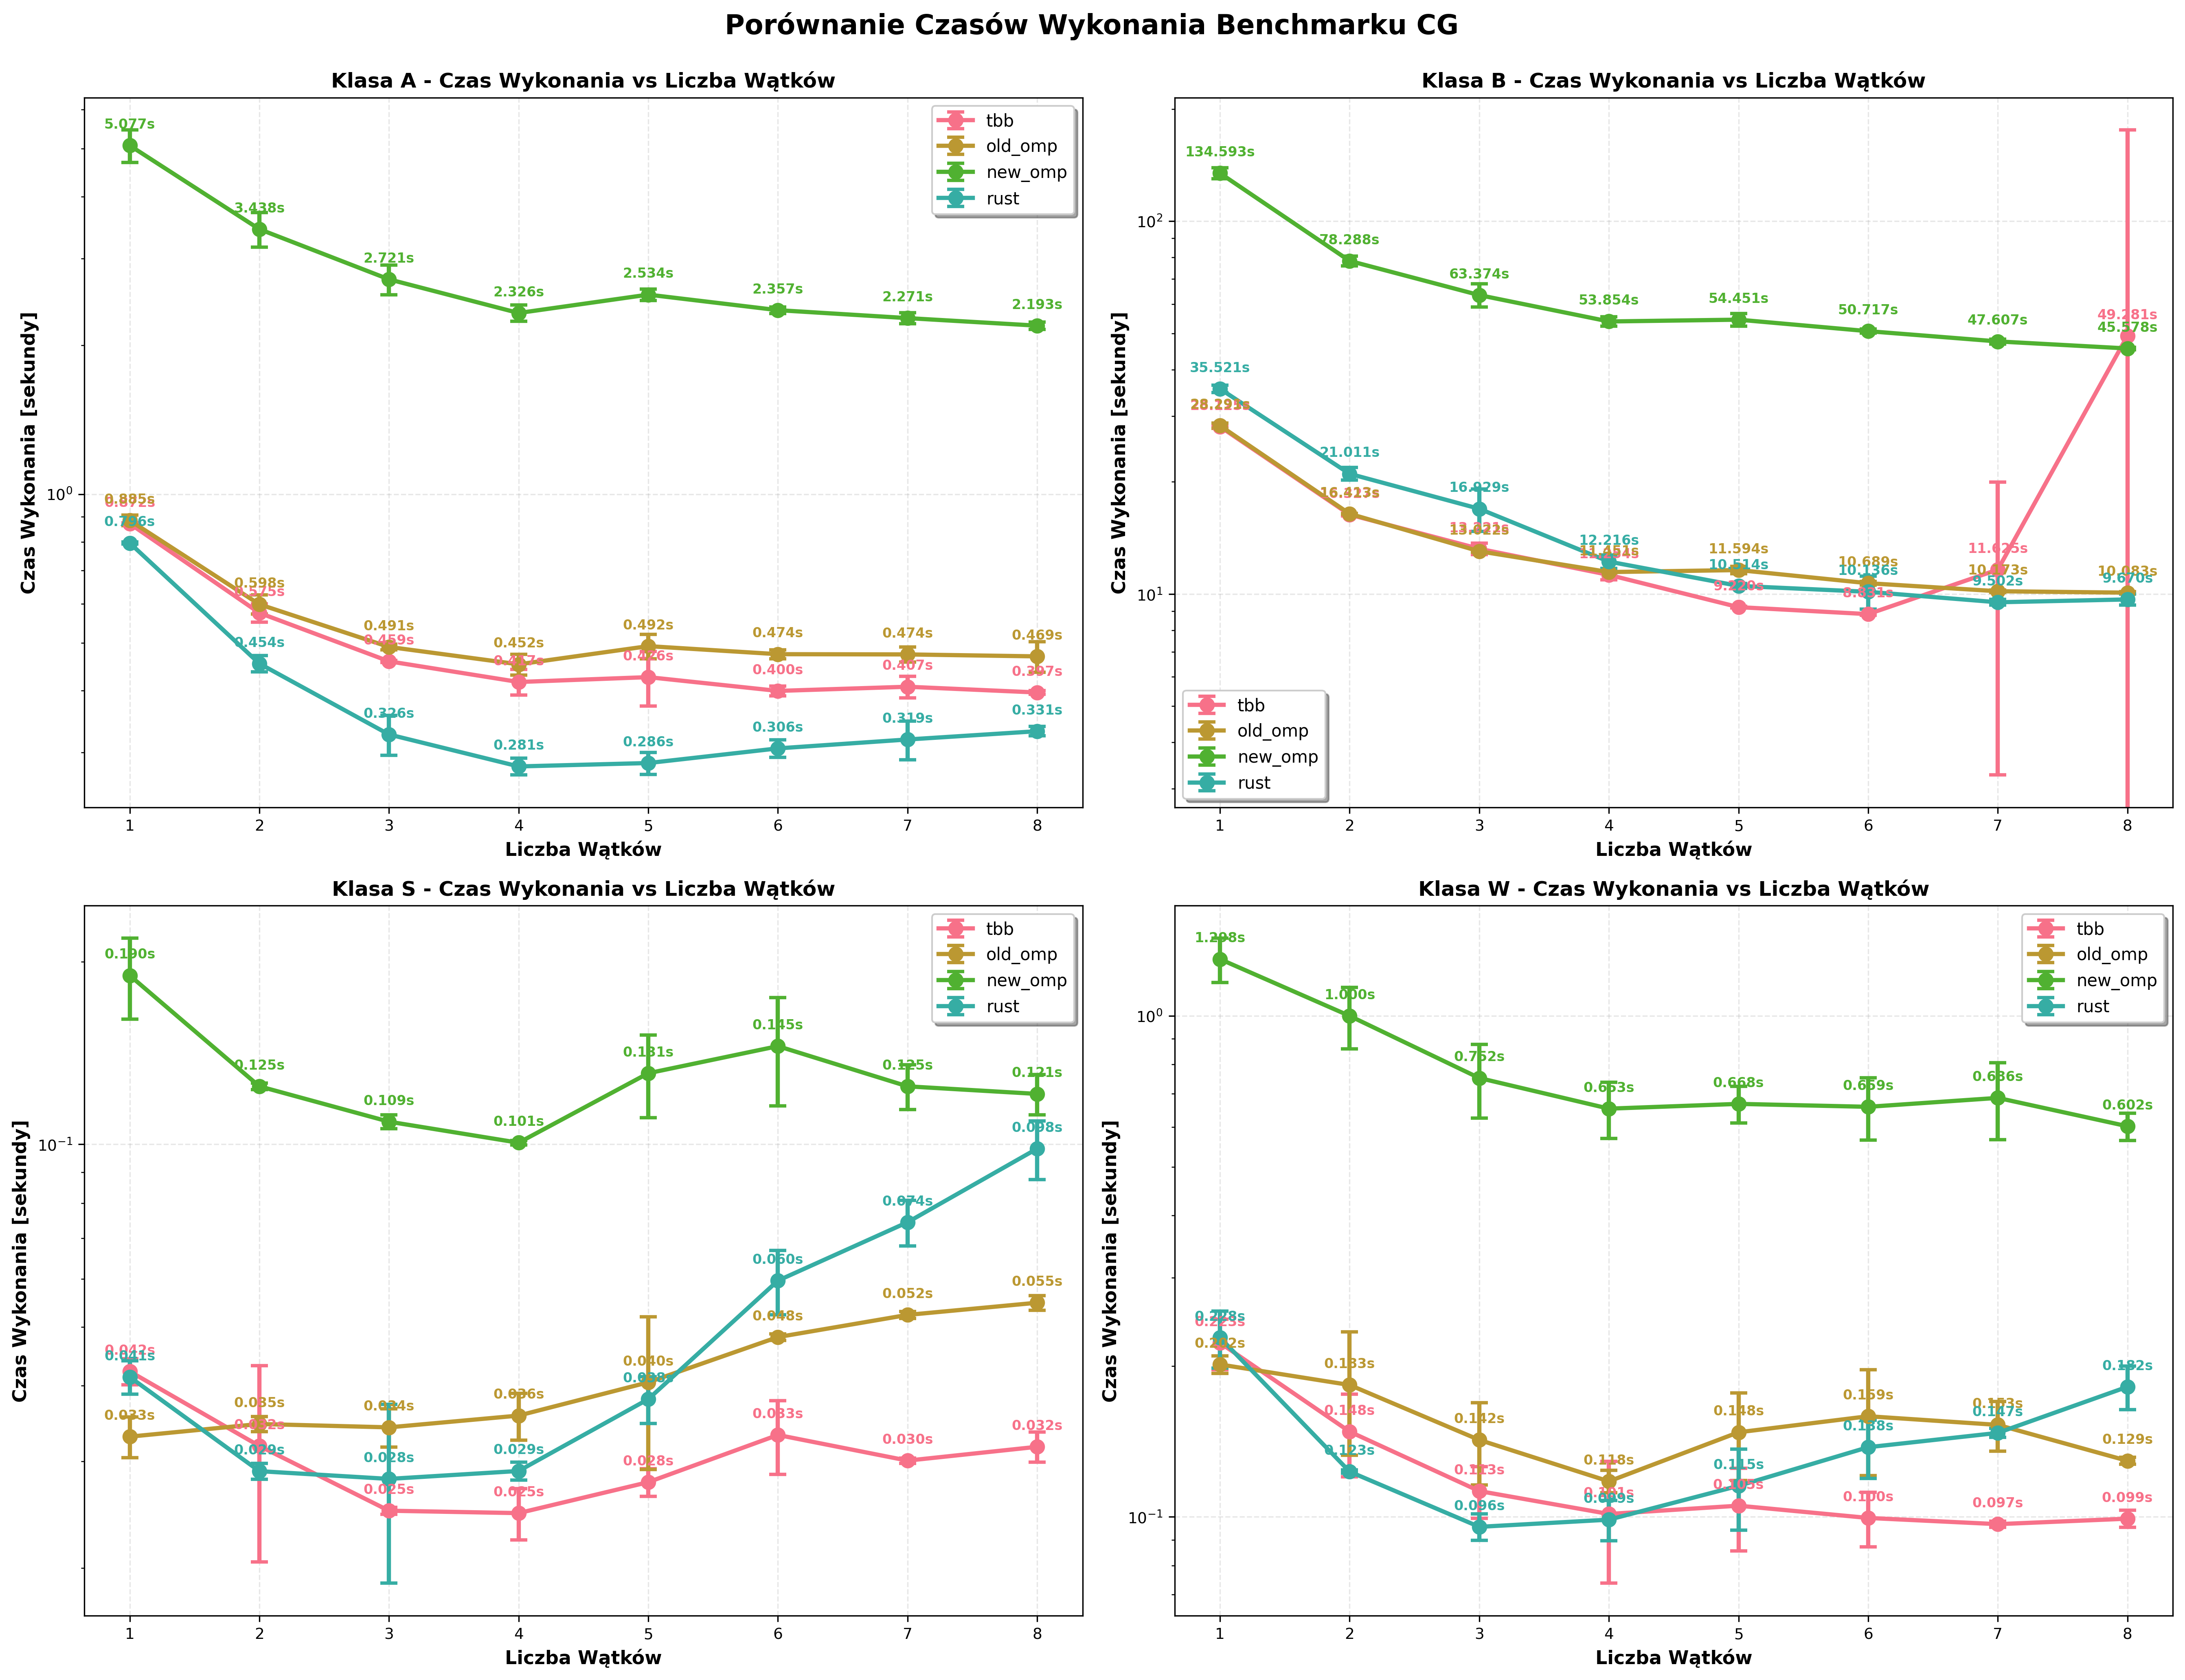
\includegraphics[width=\textwidth]{analiza/images/parallel/cg/arm/cg_porownanie_czasow_wykonania.png}
    \caption{Porównanie czasów wykonania benchmarku CG dla klas S, W, A, B względem liczby użytych wątków na platformie ARM64}
    \label{cg_porownanie_czasow_wykonania}
\end{figure}

Na rysunku \ref{cg_porownanie_czasow_wykonania} zaprezentowano zestawienie czasów wykonania benchmarku CG dla czterech klas problemu: S, W, A oraz B, przy użyciu czterech różnych implementacji równoległości: TBB, OpenMP w wersji oryginalnej w stylu języka Fortran (old\_omp), OpenMP w wersji nowszej (new\_omp) oraz implementacji w języku Rust. Dla każdej z klas przedstawiono zależność czasu wykonania od liczby wątków (od 1 do 8). Wartości zostały zaprezentowane w skali logarytmicznej.\\
Analiza czasów wykonania algorytmu CG ujawnia wyraźne różnice w wydajności poszczególnych implementacji, z dominującym problemem dotyczącym new\_omp. Najbardziej uderzającą obserwacją jest znacząco gorsza wydajność tej implementacji we wszystkich klasach problemu. Czasy wykonania new\_omp są wielokrotnie - nawet dziesięciokrotnie - dłuższe w porównaniu z pozostałymi rozwiązaniami. Dysproporcja ta jest szczególnie wyraźna w klasach A i B, gdzie new\_omp operuje w zakresie sekund, podczas gdy inne implementacje osiągają czasy rzędu dziesiątych części sekundy. Może to wskazywać na fundamentalne niedociągnięcia nowej wersji OpenMP w kontekście testowanego algorytmu, potencjalnie wynikające z nieefektywnej dekompozycji zadań lub kosztownych mechanizmów synchronizacji.

Pozostałe implementacje prezentują bardziej zbliżone wyniki, z pewnymi zauważalnymi różnicami. W klasie A, implementacja Rust wykazuje najlepsze czasy wykonania przy większej liczbie wątków (4-8), osiągając około 0,28-0,33 sekundy. W klasie B różnice są minimalne - wszystkie trzy implementacje (tbb, old\_omp, rust) osiągają porównywalne wartości rzędu 0,09-0,10 sekundy przy większej liczbie wątków. Warto jednak zauważyć istotną niestabilność czasów wykonania dla implementacji tbb przy 8 wątkach, co sygnalizuje duży rozrzut wyników. W mniejszych klasach problemowych - S i W - tbb często okazuje się najszybszą implementacją, zwłaszcza przy średnim poziomie równoległości (3-6 wątków).

Analizując wzorce skalowania, wszystkie implementacje wykazują wzrost wydajności przy przejściu z 1 do 3-4 wątków. Powyżej tego progu obserwuje się tendencję do stabilizacji lub wręcz nieznacznego pogorszenia wydajności, co może być związane z narzutami na synchronizację oraz ograniczeniami sprzętowymi. Szczególnie pozytywnie wyróżnia się tu implementacja Rust w klasie A, która prezentuje najbardziej stabilny i przewidywalny wzorzec skalowania. W pozostałych klasach implementacja ta wykazuje większą nieregularność.

\begin{figure}[H]
    \centering
    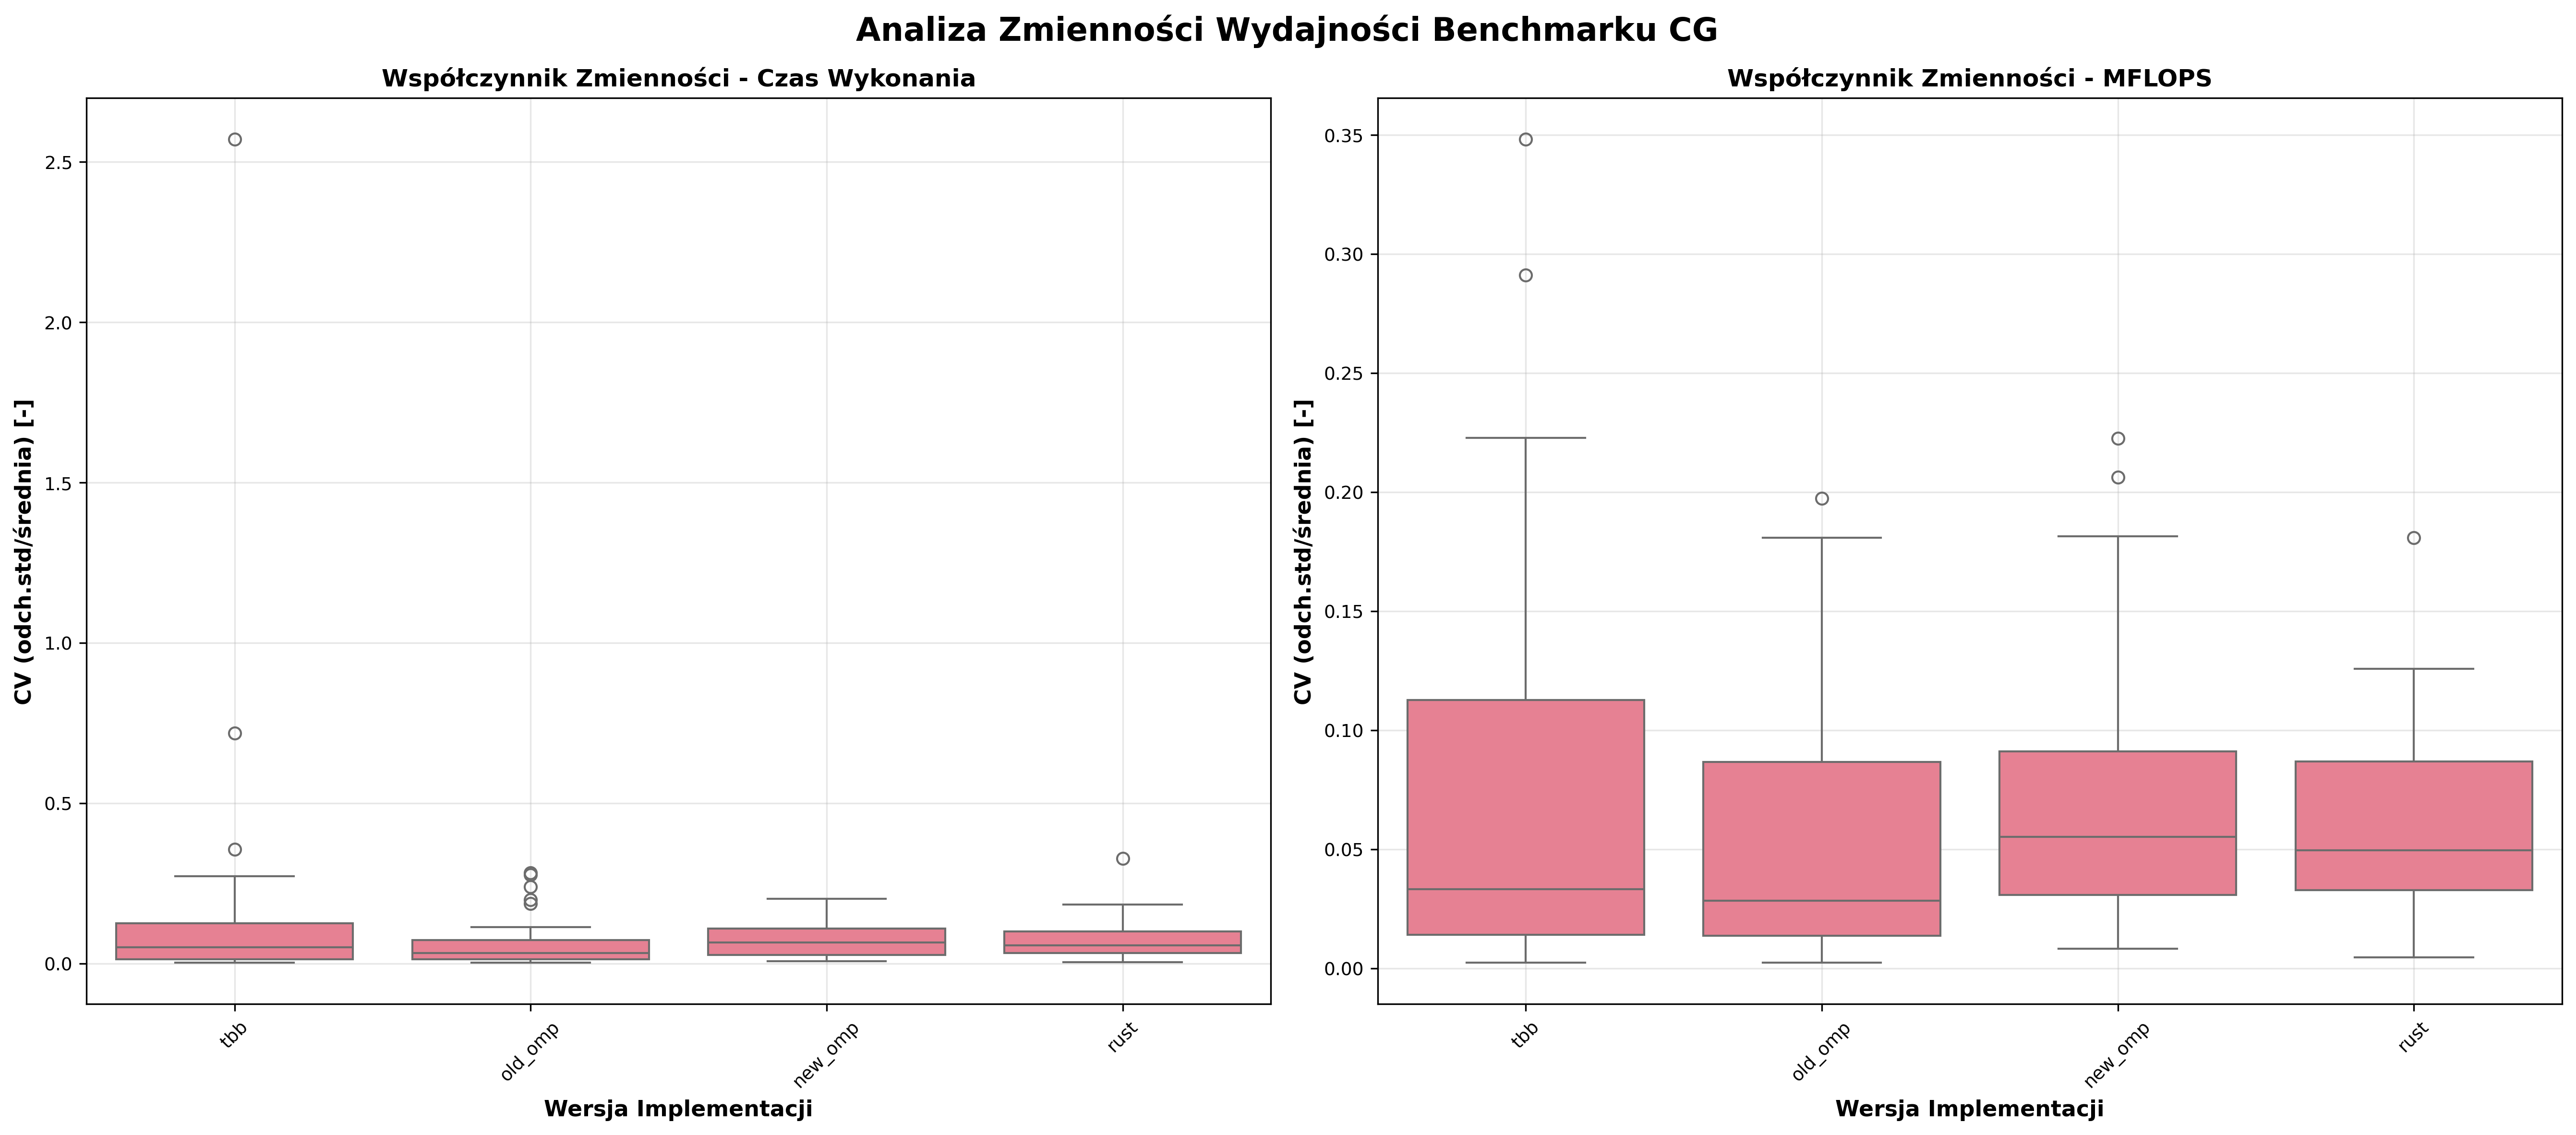
\includegraphics[width=\textwidth]{analiza/images/parallel/cg/arm/cg_analiza_zmiennosci.png}
    \caption{Analiza zmienności czasów wykonania benchmarku CG dla klas S, W, A, B względem liczby użytych wątków na platformie ARM64}
    \label{cg_analiza_zmiennosci}
\end{figure}
Powyższy wykres - rysunek \ref{cg_analiza_zmiennosci} pudełkowy prezentuje współczynnik zmienności \eng{CV - coefficient of variation}, obliczony jako stosunek odchylenia standardowego do wartości średniej, w odniesieniu do czasu wykonania (lewy wykres) oraz uzyskiwanej wydajności (prawy wykres) dla różnych wersji implementacji benchmarku.\\
Ogólnie rzecz biorąc, czasy wykonania cechują się niską zmiennością - mediana CV dla wszystkich implementacji mieści się w przedziale 0,05-0,10, co świadczy o dobrej powtarzalności wyników. Na tym tle wyróżnia się old\_omp, który osiąga najniższy poziom zmienności, sygnalizując wysoką stabilność działania. Z kolei tbb, mimo niskiej mediany, wykazuje wartości odstające, z ekstremalnymi przypadkami CV przekraczającymi 2,5.

Zmienność wartości MFLOPS jest wyraźnie wyższa niż czasów wykonania, co sugeruje, że mimo podobnych czasów działania, efektywność obliczeniowa może się znacznie wahać. Największe odchylenia obserwuje się ponownie dla implementacji tbb, gdzie wartości CV sięgają nawet 0,35. Rust wyróżnia się najbardziej konsekwentnym profilem zmienności, z wąskim zakresem rozrzutu wyników, co może wskazywać na dobrze zoptymalizowany model obliczeń wewnętrznych.

Z punktu widzenia poszczególnych klas problemowych, klasy A i B - reprezentujące większe zbiory danych - wykazują najczytelniejsze i najbardziej regularne wzorce skalowania. To właśnie w tych klasach ujawniają się największe bezwzględne różnice w czasach wykonania między implementacjami, a korzyści z równoległości są najbardziej wyraźne. W przeciwieństwie do nich, klasy S i W - charakteryzujące się mniejszymi rozmiarami danych - wykazują większą względną zmienność wyników i mniej przewidywalne zyski z równoległego przetwarzania. Nieregularne wzorce wydajności oraz większe odchylenia wskazują, że dla małych problemów korzyści z wielowątkowości są mniej oczywiste i bardziej zależne od szczegółów implementacyjnych.
%------------------------------

\begin{figure}[H]
    \centering
    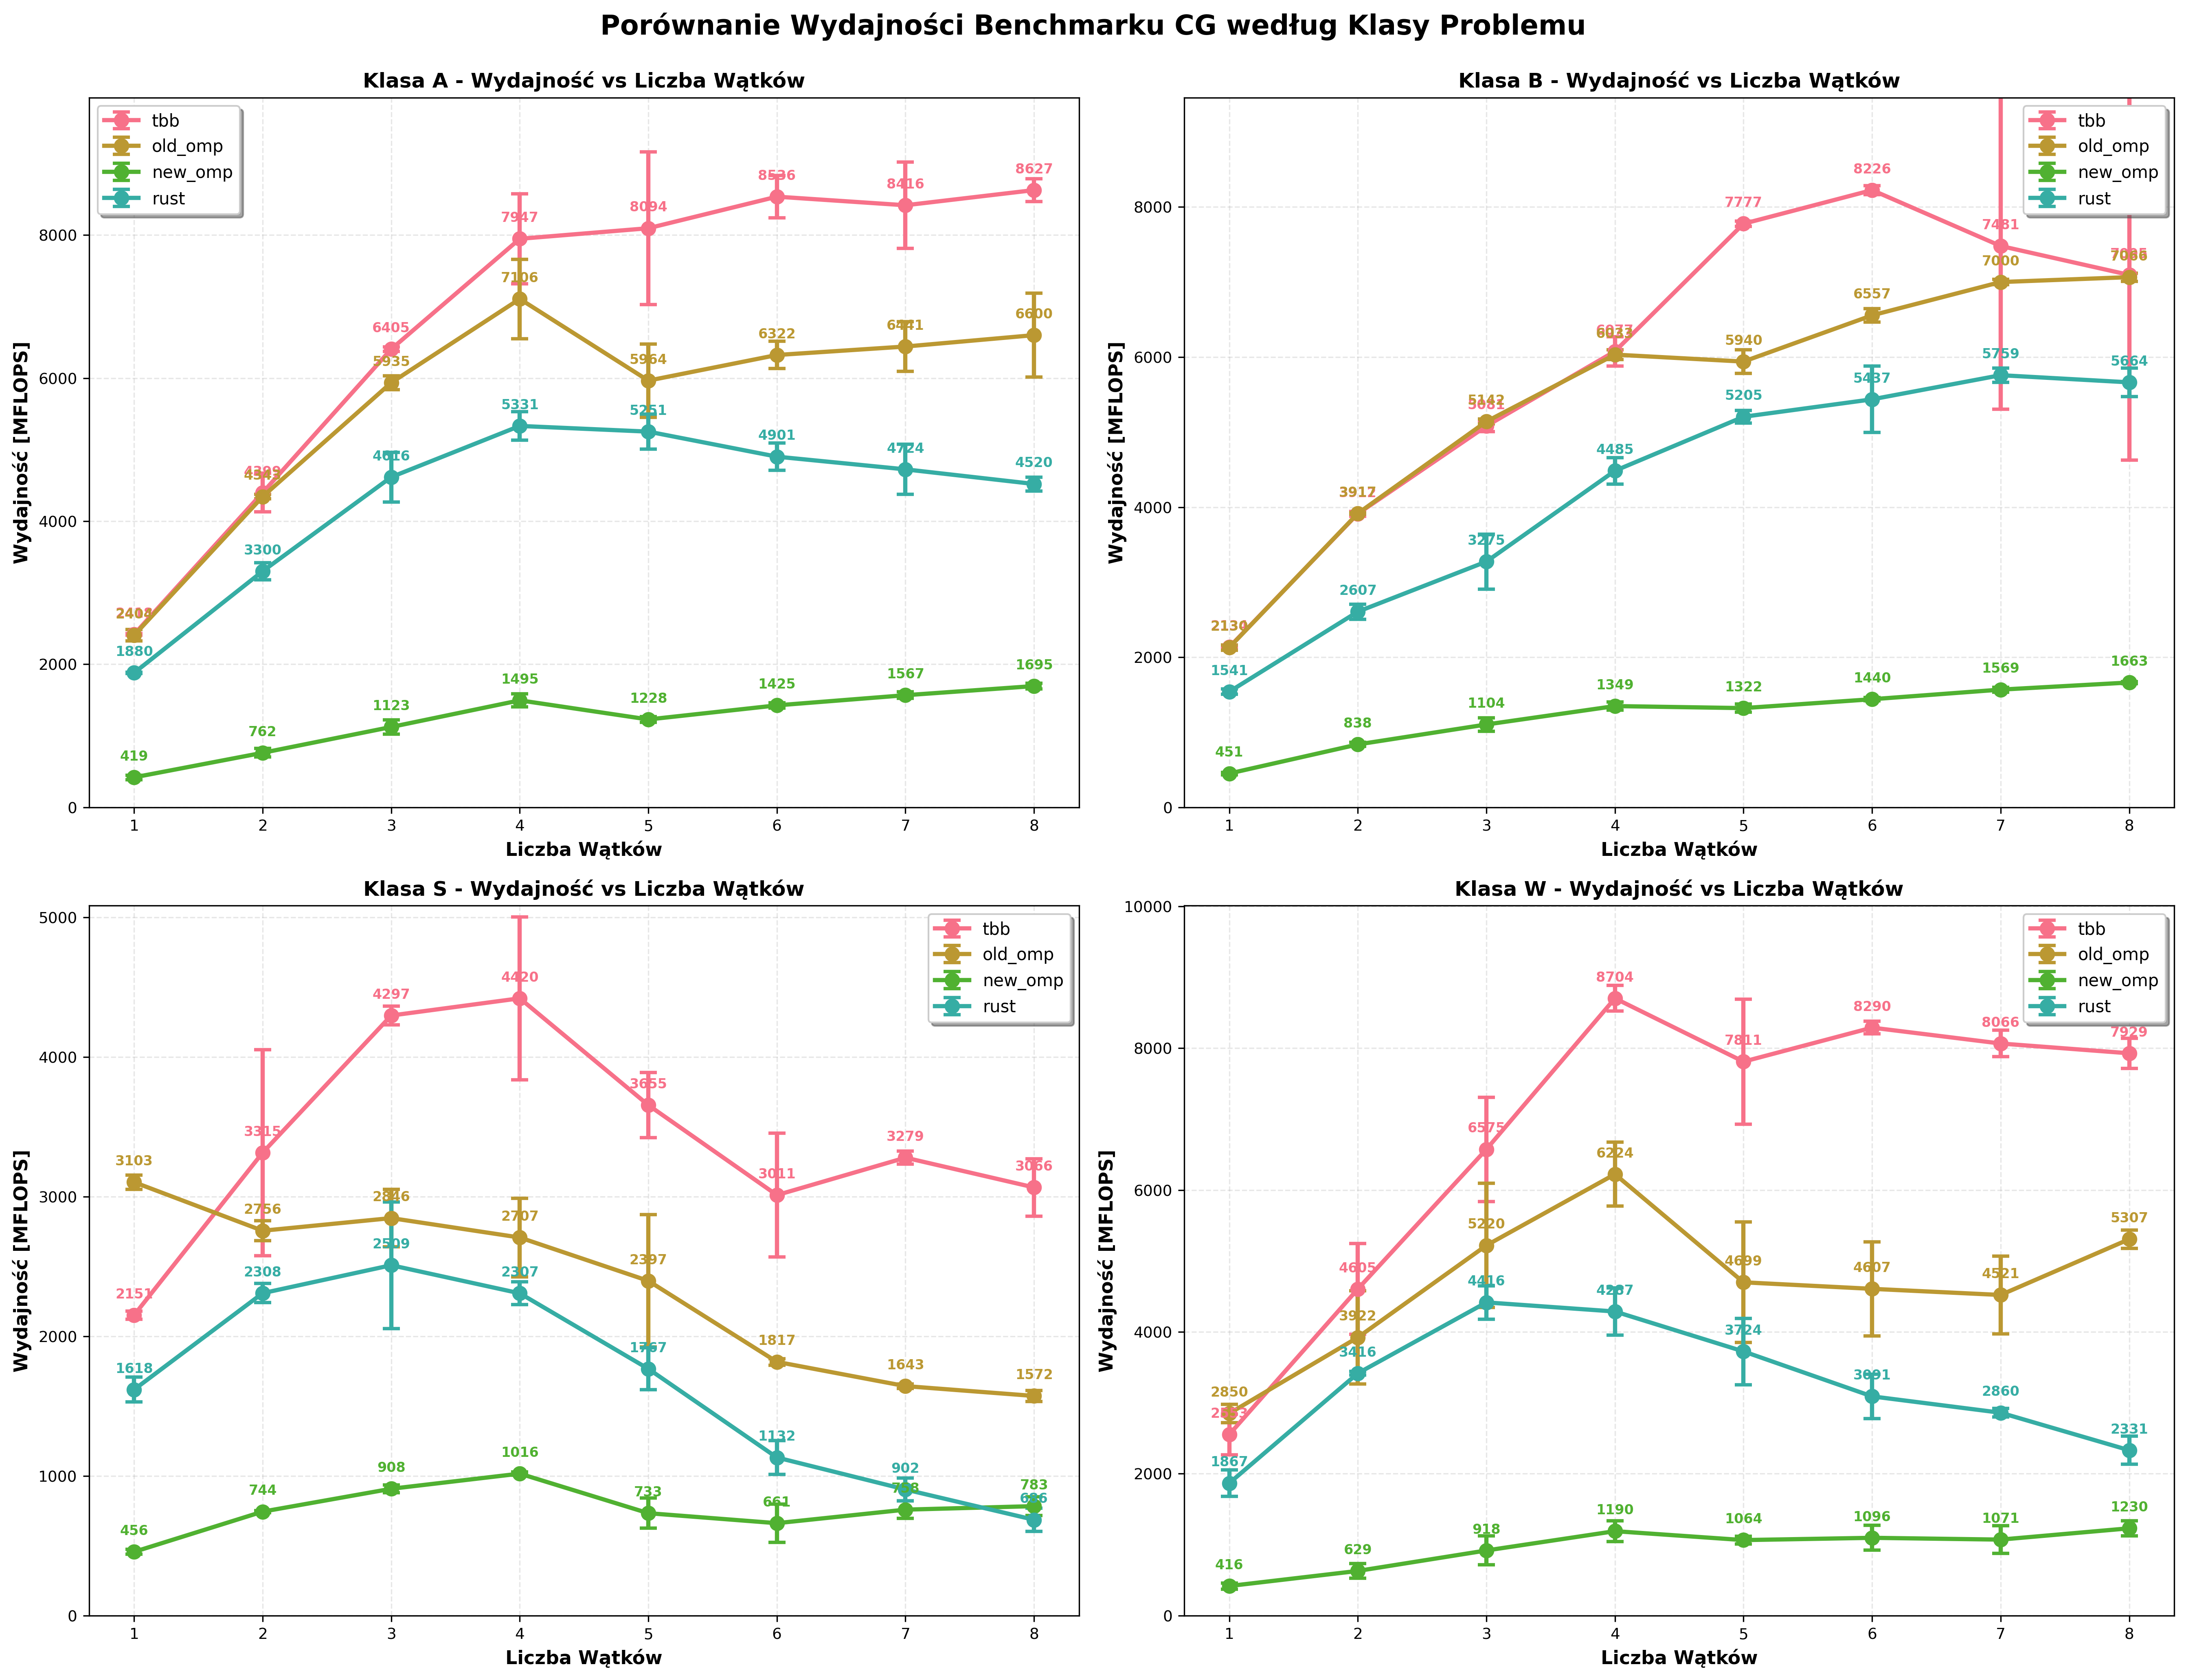
\includegraphics[width=\textwidth]{analiza/images/parallel/cg/arm/cg_porownanie_wydajnosci.png}
    \caption{Porównanie wydajności benchmarku CG dla klas S, W, A, B względem liczby użytych wątków na platformie ARM64}
    \label{cg_porownanie_wydajnosci}
\end{figure}
Na wykresach na rysunku \ref{cg_porownanie_wydajnosci} zaprezentowano porównanie wydajności benchmarku CG mierzonej w MFLOPS (milionach operacji zmiennoprzecinkowych na sekundę). Wydajność została przedstawiona jako funkcja liczby wątków (1-8) dla czterech implementacji równoległych.

\subsubsection{Analiza trendów wydajnościowych}
Implementacja oparta na bibliotece Intel TBB konsekwentnie wykazuje najwyższą wydajność we wszystkich klasach problemów, osiągając szczytowe wartości MFLOPS (miliony operacji zmiennoprzecinkowych na sekundę) przy wykorzystaniu 3-6 wątków. Szczególnie widoczna jest jej przewaga w klasach A, B i W, gdzie osiąga wartości przekraczające 8000 MFLOPS.

Implementacja OpenMP w starszej wersji (old\_omp) plasuje się na drugiej pozycji pod względem wydajności, osiągając wyniki o około 20-30\% niższe niż TBB. Wykazuje ona podobny charakter skalowania, jednak z mniejszą efektywnością przy większej liczbie wątków.

Implementacja w języku Rust prezentuje umiarkowaną wydajność, osiągając wyniki zbliżone do old\_omp w niektórych konfiguracjach, jednak generalnie niższe. Warto zauważyć, że w klasie S wykazuje ona znaczący spadek wydajności powyżej 4 wątków.

Implementacja OpenMP w nowszej wersji (new\_omp) osiąga konsekwentnie najniższe wyniki wydajności spośród wszystkich testowanych wariantów, z wartościami MFLOPS kilkukrotnie niższymi od lidera.

\subsubsection{Charakterystyka skalowania}
Większość implementacji osiąga szczytową wydajność przy wykorzystaniu 3-4 wątków, po czym następuje stabilizacja lub nawet spadek wydajności. Zjawisko to jest szczególnie wyraźne w klasie S, gdzie wszystkie implementacje wykazują znaczący spadek wydajności przy większej liczbie wątków, co sugeruje, że problemy tej klasy cechują się wysokim stosunkiem komunikacji do obliczeń.

Klasy A i B wykazują podobne charakterystyki skalowania, z wyraźnym wzrostem wydajności do około 4 wątków i późniejszym wypłaszczeniem. Klasa W charakteryzuje się podobnym trendem, jednak z większymi fluktuacjami wydajności.

\begin{figure}[H]
    \centering
    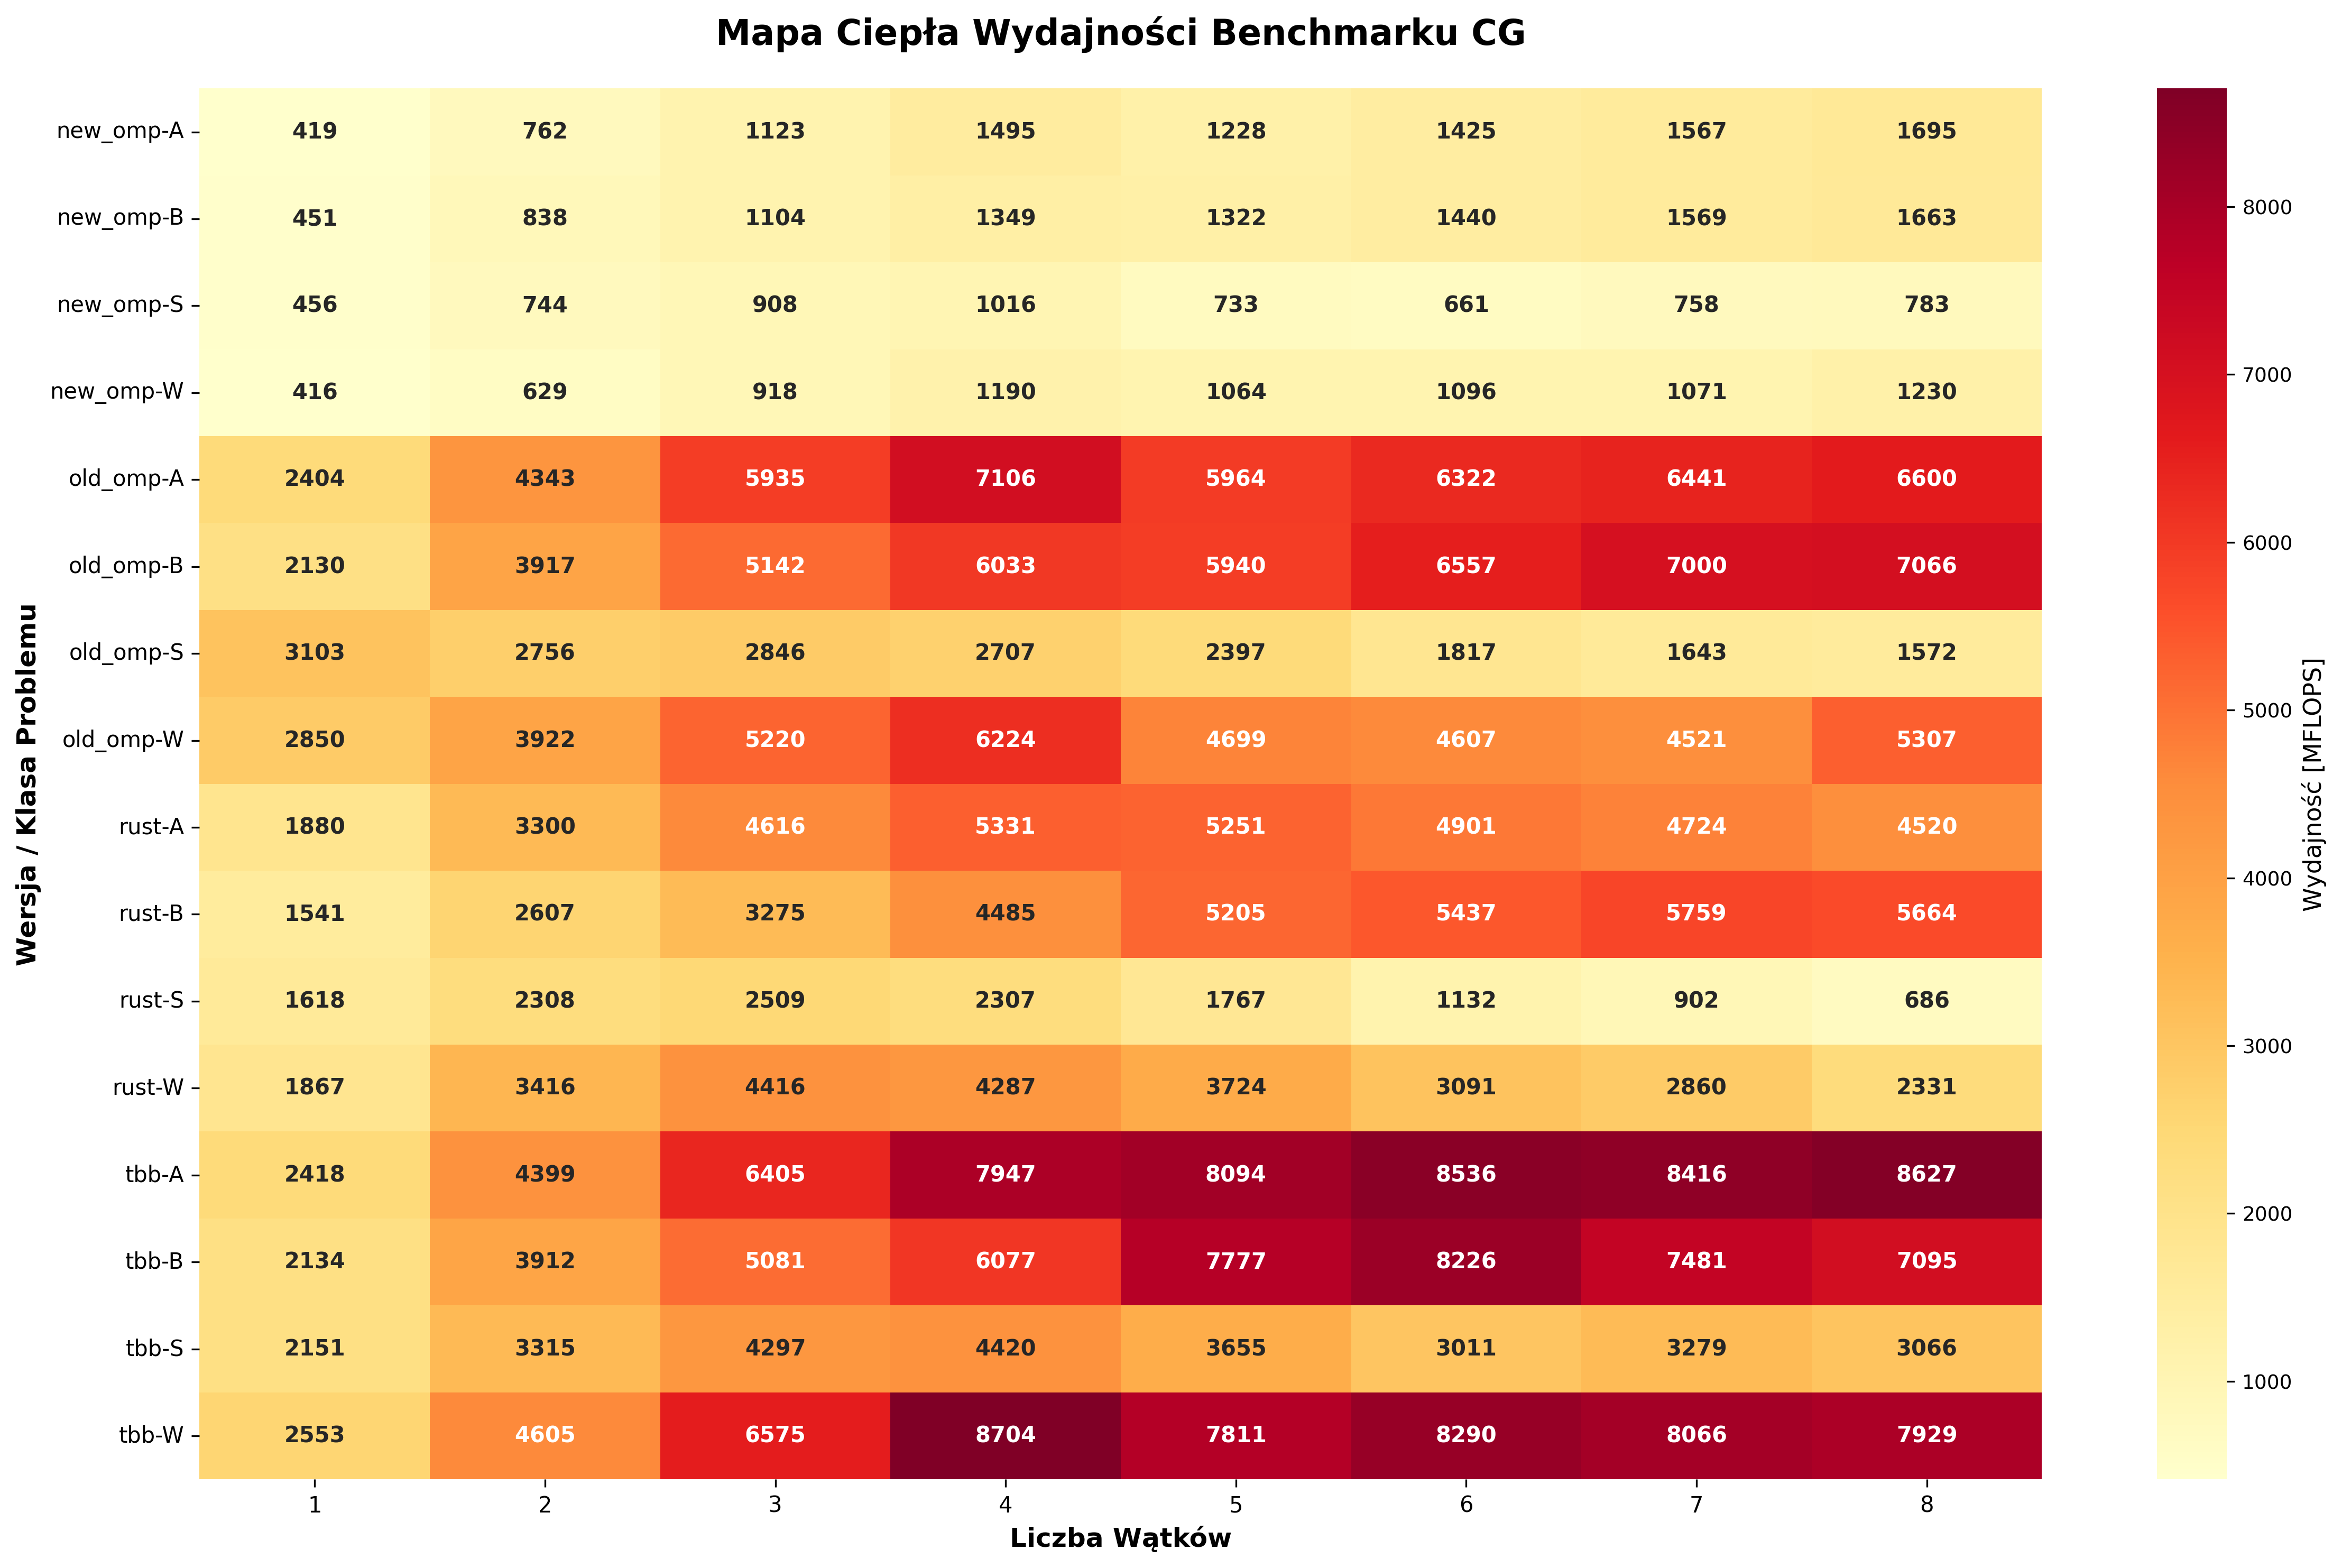
\includegraphics[width=\textwidth]{analiza/images/parallel/cg/arm/cg_mapa_ciepla_wydajnosci.png}
    \caption{Mapa ciepła wydajności benchmarku CG dla klas S, W, A, B względem liczby użytych wątków na platformie ARM64}
    \label{cg_heatmap_wydajnosci}
\end{figure}
Mapa ciepła wydajności - rysunek \ref{cg_heatmap_wydajnosci} potwierdza powyższe obserwacje, dostarczając kompleksowego widoku na zachowanie wszystkich implementacji w funkcji klasy problemu i liczby wątków. Najwyższe wartości wydajności (reprezentowane cieplejszymi, czerwonymi odcieniami) koncentrują się w obszarze implementacji TBB dla klas A, B i W przy liczbie wątków 3-8. Zimniejsze obszary mapy (żółte i jasnożółte) odpowiadają konsekwentnie implementacji new\_omp dla wszystkich klas problemów.

Zauważalny jest również gradient wydajności w przypadku klasy S, gdzie wszystkie implementacje wykazują wyraźny spadek wydajności wraz ze wzrostem liczby wątków powyżej wartości optymalnej (3-4), co manifestuje się przejściem od cieplejszych do chłodniejszych odcieni w prawej części mapy ciepła.


\begin{figure}[H]
    \centering
    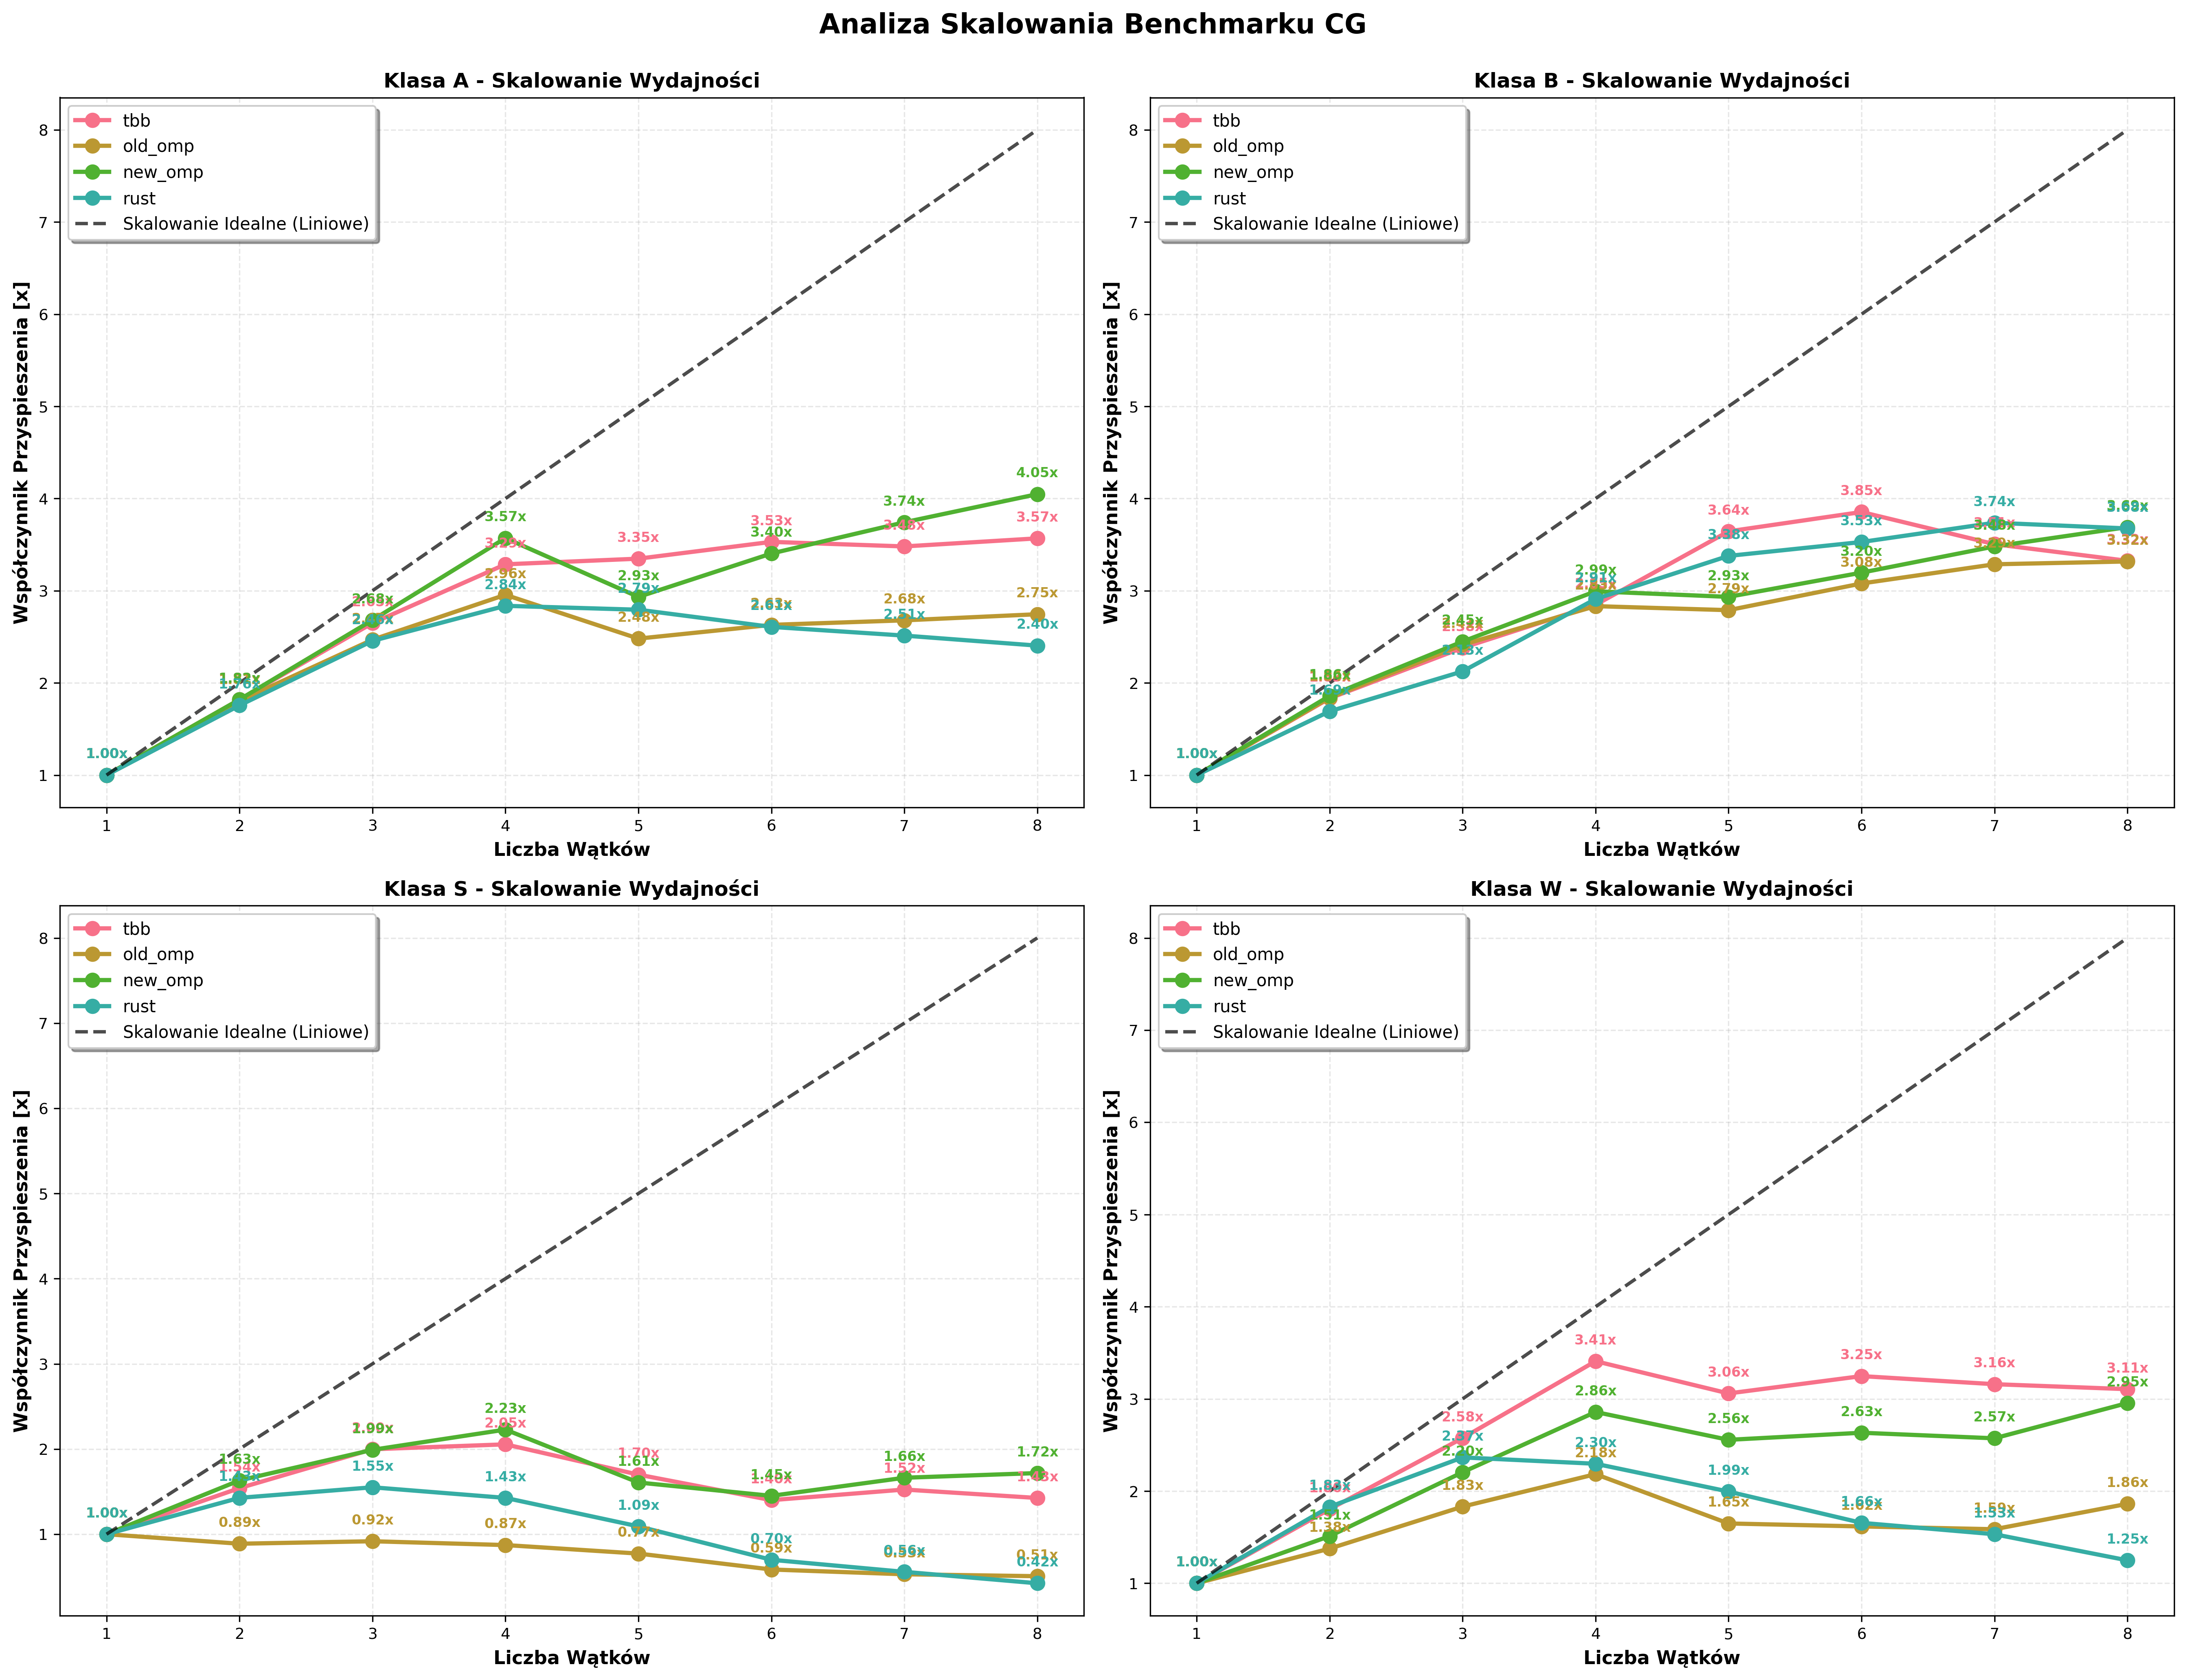
\includegraphics[width=\textwidth]{analiza/images/parallel/cg/arm/cg_analiza_skalowania.png}
    \caption{Analiza skalowania benchmarku CG dla klas S, W, A, B względem liczby użytych wątków na platformie ARM64}
    \label{cg_analiza_skalowania}
\end{figure}
Powyższy wykres - rysunek \ref{cg_analiza_skalowania} przedstawia skalowanie wydajności benchmarku CG. Skalowanie wyrażone zostało za pomocą współczynnika przyspieszenia względem wykonania jednowątkowego i odniesione do skalowania idealnego (liniowego).

\subsubsection{Analiza porównawcza implementacji}
Żadna z badanych implementacji nie osiąga idealnego skalowania liniowego, co wskazuje na istnienie inherentnych ograniczeń w równoległym wykonaniu algorytmu CG. Większość implementacji osiąga punkt maksymalnego przyspieszenia przy wykorzystaniu 3-4 wątków, po czym efektywność skalowania ulega wyraźnemu spłaszczeniu lub nawet spadkowi. Zjawisko to można przypisać rosnącym kosztom synchronizacji, kontencji pamięci podręcznej oraz ograniczeniom przepustowości pamięci.

Implementacja Intel TBB wykazuje generalnie najlepsze charakterystyki skalowania w większości klas problemów, szczególnie widoczne w klasach A, B i W. W optymalnym przypadku osiąga przyspieszenie rzędu 3,0-3,6x przy wykorzystaniu 4-5 wątków. Implementacja ta wykazuje najwyższą efektywność równoległą, co może świadczyć o skutecznych mechanizmach zarządzania zadaniami i minimalizacji narzutu synchronizacji.

Implementacja OpenMP w nowszej wersji prezentuje interesującą charakterystykę skalowania, osiągając w klasie problemu A najwyższe zaobserwowane przyspieszenie około 4,5x przy 8 wątkach. Wynik ten sugeruje, że nowa implementacja OpenMP może efektywniej wykorzystywać zasoby obliczeniowe w przypadku określonych wzorców dostępu do pamięci.

Starsza implementacja OpenMP wykazuje umiarkowane skalowanie w klasach A i B, jednak znacząco gorsze w klasie S, gdzie przyspieszenie pozostaje minimalne niezależnie od liczby wątków. Wskazuje to na potencjalne problemy w obsłudze problemów o wysokim stosunku komunikacji do obliczeń.

Implementacja w języku Rust cechuje się początkowym wzrostem wydajności, który szybko ulega nasyceniu, a przy wyższej liczbie wątków często obserwuje się spadek przyspieszenia. Szczególnie widoczne jest to w klasie S, gdzie przy 7-8 wątkach współczynnik przyspieszenia spada poniżej 1,0, co oznacza degradację wydajności względem wykonania jednowątkowego.

\subsubsection{Wpływ klasy problemu na skalowanie}
Klasy problemów A i B wykazują zbliżone charakterystyki skalowania dla wszystkich badanych implementacji, co sugeruje podobne właściwości dostępu do pamięci i intensywności obliczeniowej.

Klasa S charakteryzuje się zdecydowanie najgorszym skalowaniem spośród wszystkich badanych klas, z maksymalnym przyspieszeniem nieprzekraczającym 2x. Wynik ten wskazuje na wysokie koszty komunikacji w stosunku do wykonywanych obliczeń lub nieefektywne wykorzystanie lokalności danych.

Klasa W prezentuje charakterystykę skalowania pośrednią między klasami A/B a klasą S, z maksymalnym przyspieszeniem w granicach 3x dla implementacji TBB.


\subsection{Wyniki benchmarków - platforma x86\_64}
\begin{figure}[H]
    \centering
    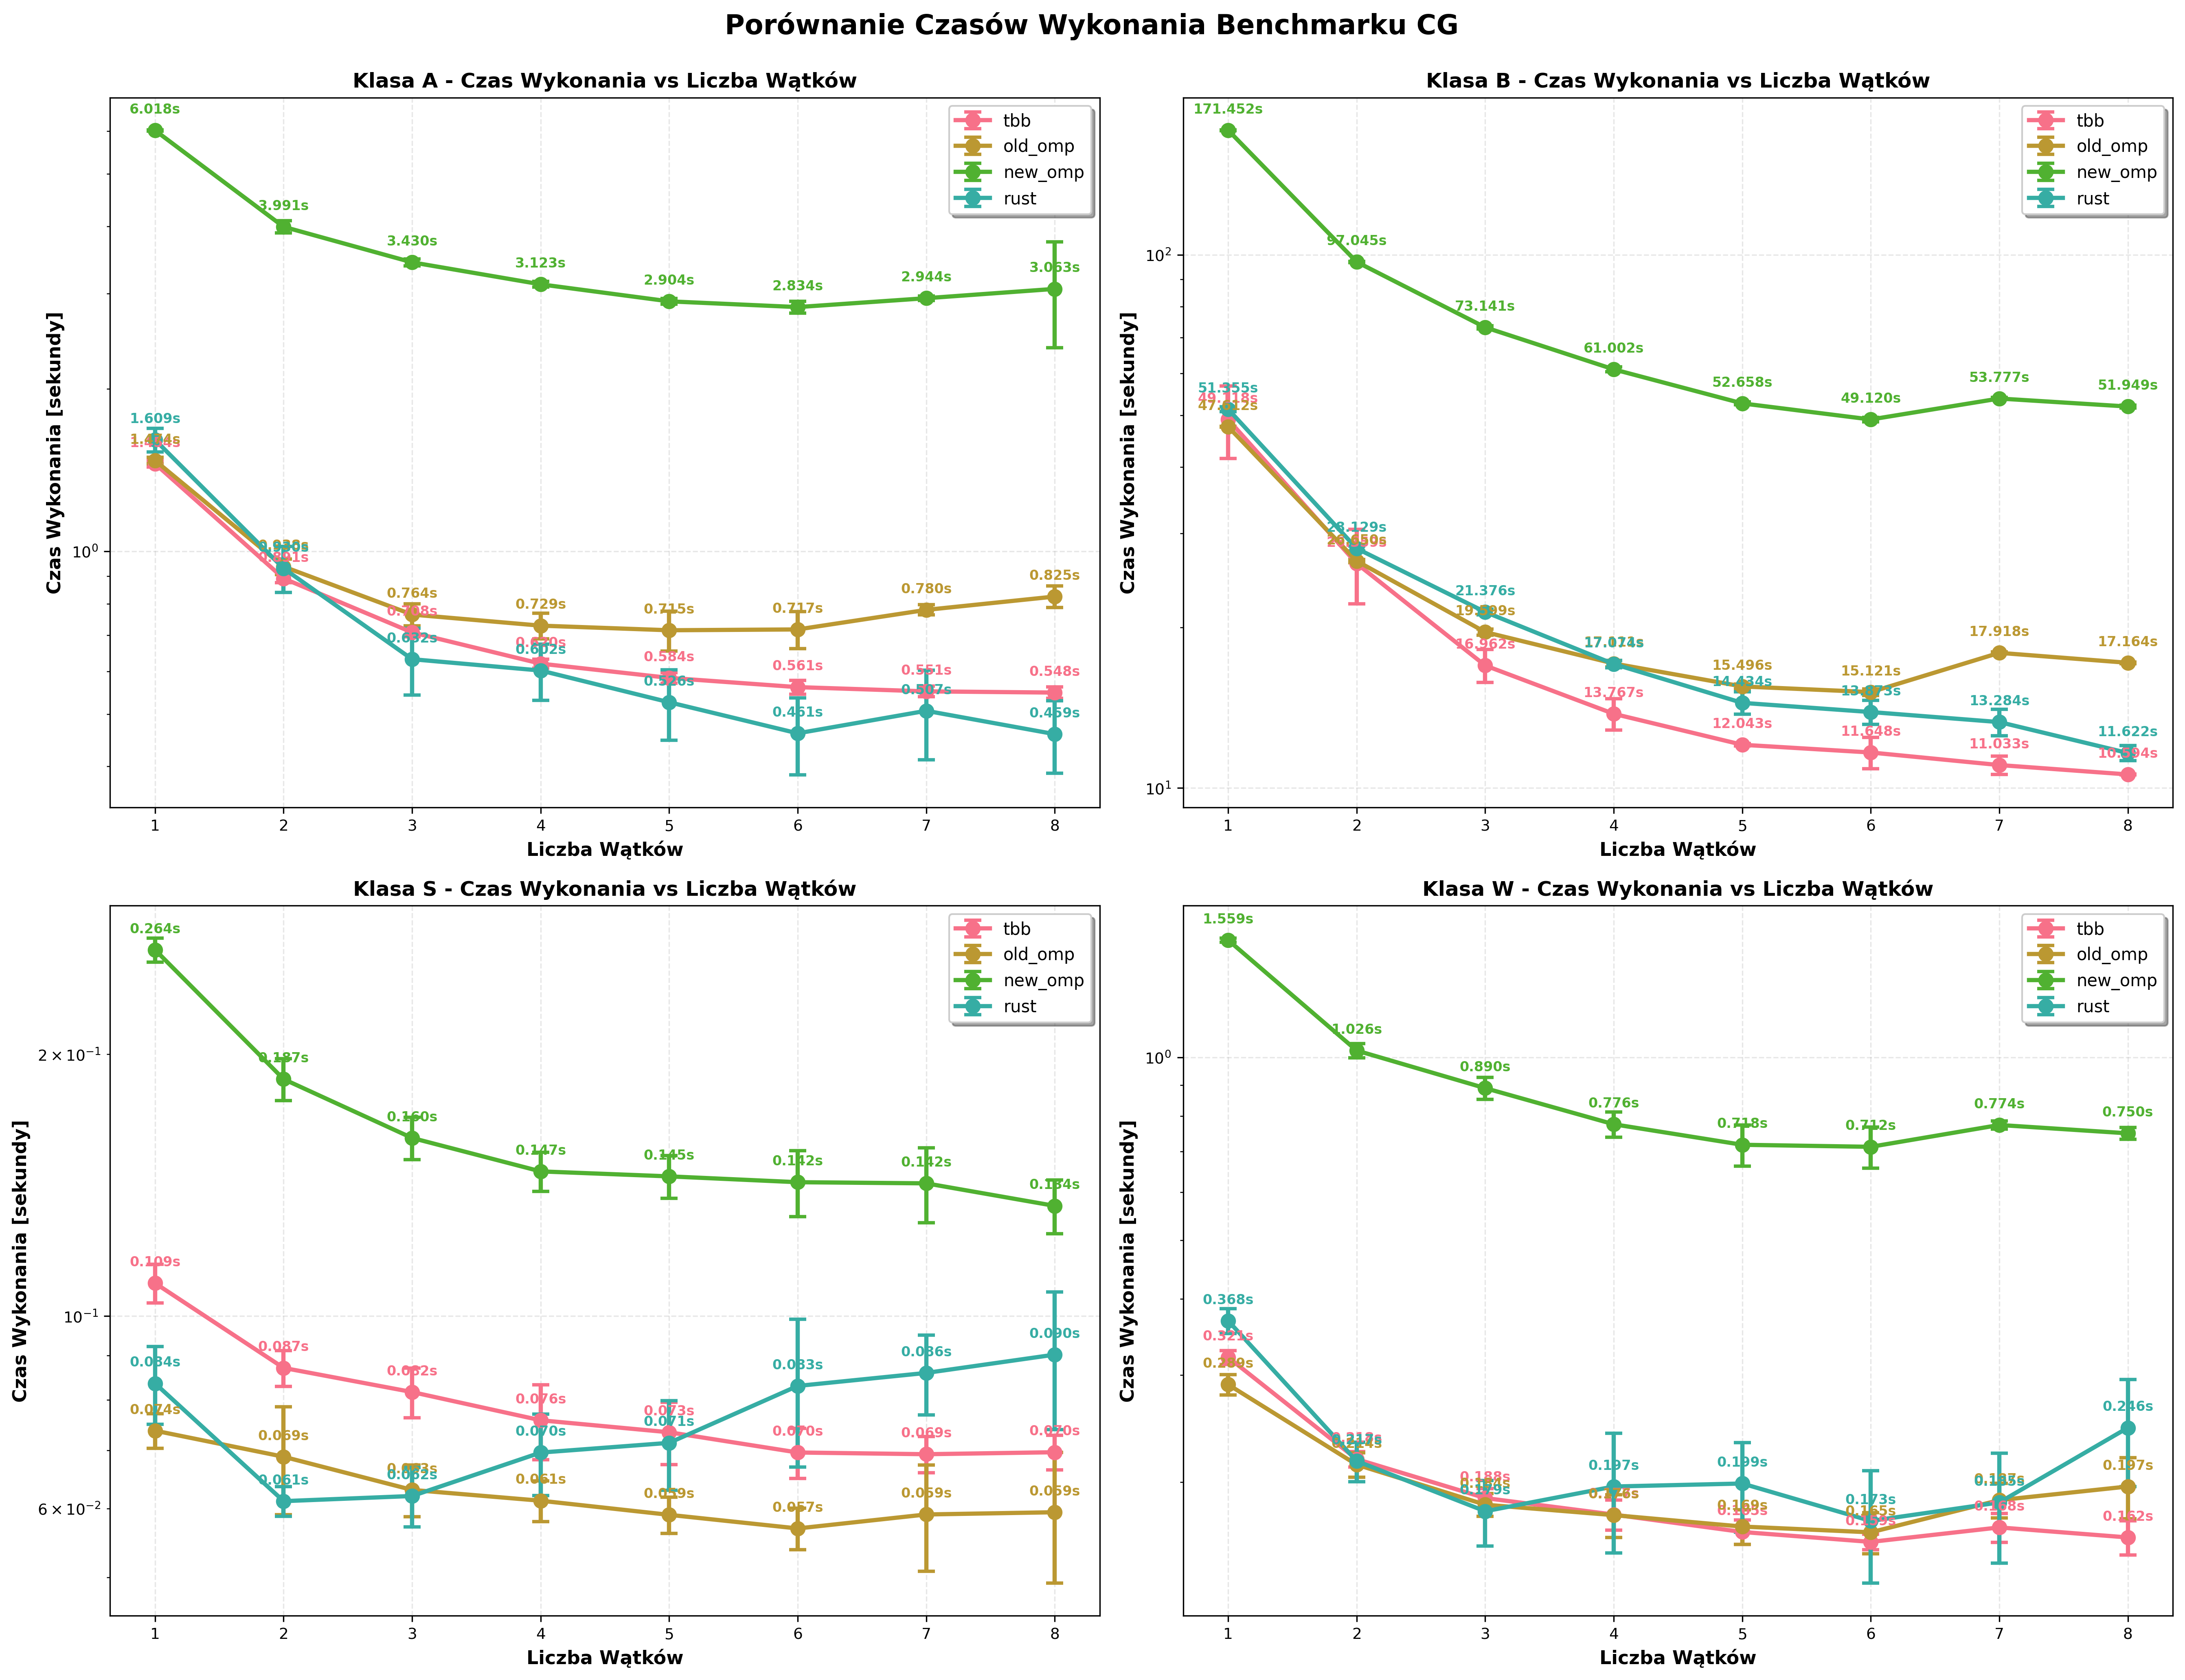
\includegraphics[width=\textwidth]{analiza/images/parallel/cg/x86/cg_porownanie_czasow_wykonania.png}
    \caption{Porównanie czasów wykonania benchmarku CG dla klas S, W, A, B względem liczby użytych wątków na platformie x86\_64}
    \label{cg_porownanie_czasow_wykonania_x86_64}
\end{figure}
Na wykresach - rysunek \ref{cg_porownanie_czasow_wykonania_x86_64} porównujących czasy wykonania poszczególnych implementacji benchmarku CG (przedstawione w skali logarytmicznej) dla czterech klas problemów (A, B, S, W), zaobserwować można wyraźne różnice w wydajności poszczególnych implementacji oraz ich skalowaniu wraz ze wzrostem liczby wątków.

Implementacja new\_omp konsekwentnie wykazuje najdłuższe czasy wykonania we wszystkich klasach problemów, z wartościami o rząd wielkości wyższymi niż pozostałe implementacje. Szczególnie widoczne jest to w klasach problemów A i B, gdzie różnica między implementacją new\_omp a pozostałymi jest najbardziej znacząca. Pomimo stosunkowo dobrej stabilności tej implementacji, jej niska wydajność czyni ją najmniej optymalnym wyborem spośród badanych wariantów.

Implementacja TBB generalnie osiąga najkrótsze czasy wykonania, zwłaszcza przy wykorzystaniu większej liczby wątków (4-8). W przypadku klasy B dla 8 wątków, implementacja TBB osiąga czas wykonania rzędu 11 milisekund, co stanowi najlepszy wynik spośród wszystkich badanych konfiguracji.

Implementacje Rust i starsza wersja OpenMP (old\_omp, kolor żółty) prezentują zbliżone charakterystyki czasów wykonania, często naprzemiennie zajmując drugą lub trzecią pozycję pod względem wydajności. W klasie problemu S można zaobserwować interesujące punkty przecięcia krzywych wydajności, gdzie implementacje zmieniają swoją relatywną efektywność w zależności od liczby wątków.

Wszystkie implementacje wykazują poprawę wydajności wraz ze wzrostem liczby wątków, jednak skala tej poprawy jest zróżnicowana. Najlepsze skalowanie obserwowane jest dla implementacji TBB, która wykazuje największy spadek czasu wykonania przy przejściu od 1 do 4 wątków. Dla większości implementacji, korzyści wynikające z dodawania kolejnych wątków powyżej 4-6 stają się marginalne, co wskazuje na osiągnięcie punktu nasycenia skalowania.

\begin{figure}[H]
    \centering
    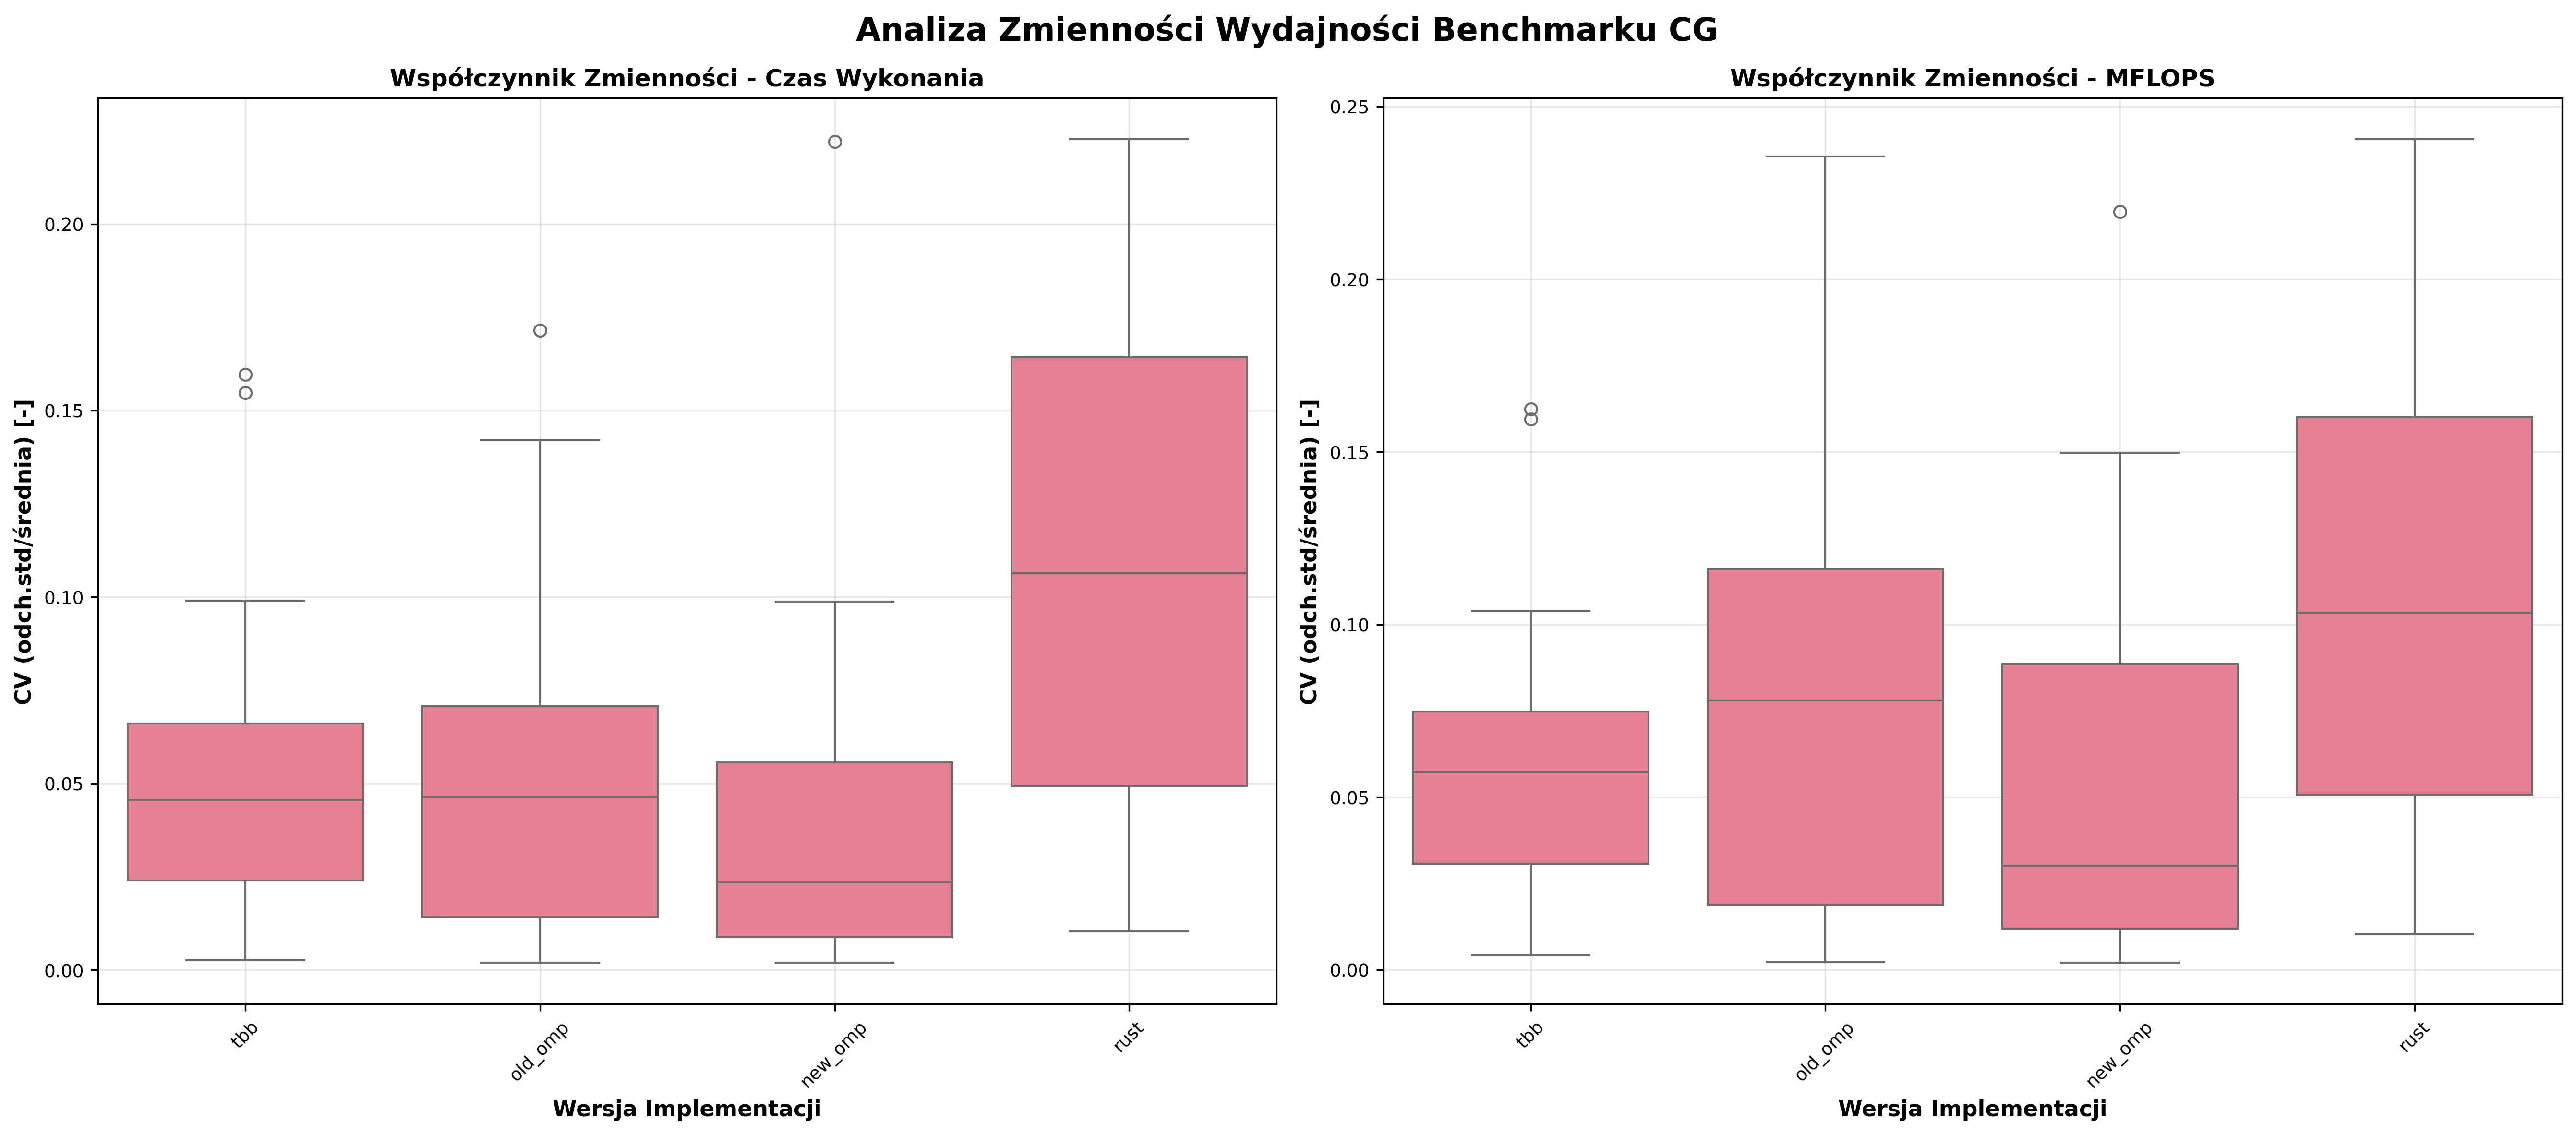
\includegraphics[width=\textwidth]{analiza/images/parallel/cg/x86/cg_analiza_zmiennosci.png}
    \caption{Analiza zmienności czasów wykonania benchmarku CG dla klas S, W, A, B względem liczby użytych wątków na platformie x86\_64}
    \label{cg_analiza_zmiennosci_x86_64}
\end{figure}
Wykresy - rysunek \ref{cg_porownanie_czasow_wykonania_x86_64} przedstawiają czasy wykonania benchmarku CG dla czterech klas problemu (A, B, S, W) w zależności od liczby wątków, dla czterech implementacji równoległych: tbb, old\_omp, new\_omp i rust.

Implementacja w języku Rust charakteryzuje się najwyższym współczynnikiem zmienności zarówno dla czasu wykonania, jak i dla wydajności MFLOPS. Mediana CV dla implementacji Rust jest znacząco wyższa niż dla pozostałych implementacji, co wskazuje na niższą przewidywalność wydajności tej implementacji. Rozstęp międzykwartylowy jest również największy dla implementacji Rust, co sugeruje większą dyspersję wyników pomiarów w porównaniu do innych wariantów.

Implementacja oparta na Intel TBB oraz starsza wersja implementacji OpenMP (old\_omp) wykazują zbliżone charakterystyki zmienności, ze średnimi wartościami CV dla czasu wykonania oscylującymi wokół 0.05. Jednocześnie implementacja new\_omp prezentuje najniższy medianowy współczynnik zmienności dla czasu wykonania, co sugeruje jej wysoką stabilność pomimo niższej wydajności bezwzględnej.

Interesującym aspektem jest obecność pojedynczych obserwacji odstających widocznych szczególnie dla implementacji new\_omp i old\_omp, które mogą wskazywać na sporadyczne zakłócenia spowodowane czynnikami zewnętrznymi lub specyficznymi przypadkami brzegowymi w algorytmie.

\begin{figure}[H]
    \centering
    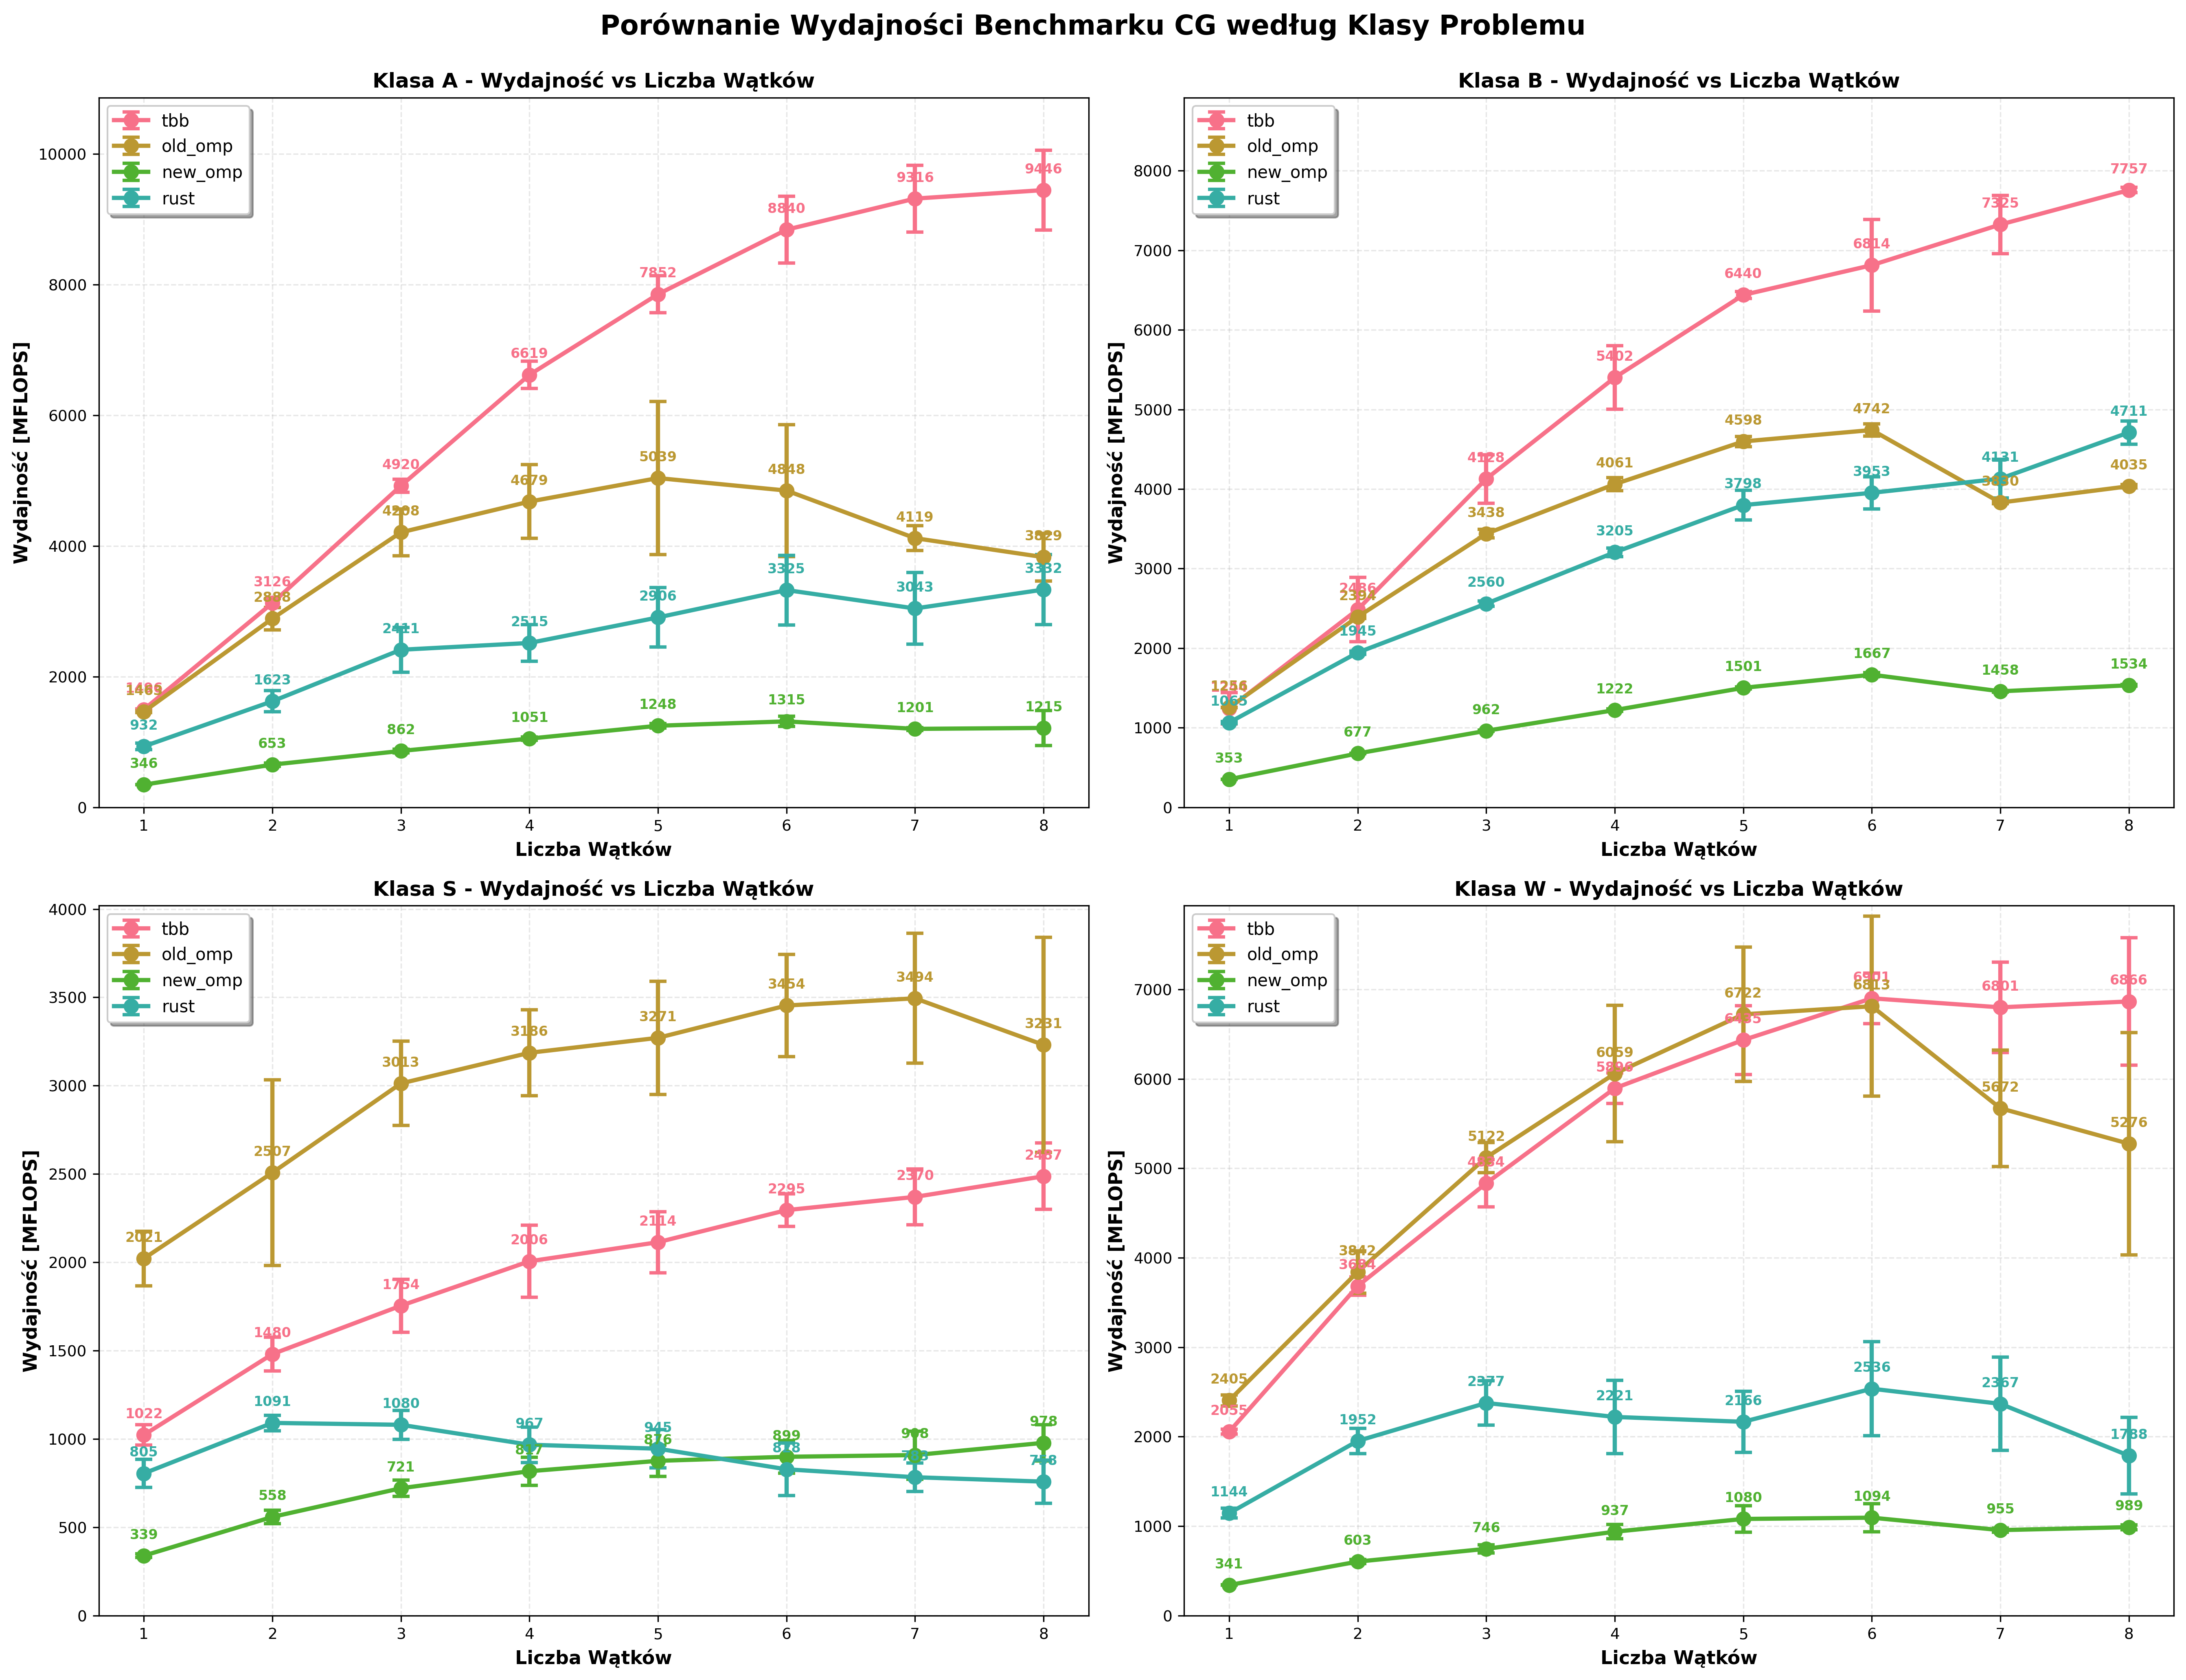
\includegraphics[width=\textwidth]{analiza/images/parallel/cg/x86/cg_porownanie_wydajnosci.png}
    \caption{Porównanie wydajności benchmarku CG dla klas S, W, A, B względem liczby użytych wątków na platformie ARM64}
    \label{cg_porownanie_wydajnosci_x86_64}
\end{figure}
Na wykresach na rysunku \ref{cg_porownanie_wydajnosci_x86_64} zaprezentowano porównanie wydajności benchmarku CG mierzonej w MFLOPS (milionach operacji zmiennoprzecinkowych na sekundę). Wydajność została przedstawiona jako funkcja liczby wątków (1-8) dla czterech implementacji równoległych.

Implementacja bazująca na bibliotece TBB, wykazuje najwyższą wydajność obliczeniową w klasach problemów A, B i W. Dla klasy A osiąga ona maksymalną wydajność przekraczającą 9400 MFLOPS przy wykorzystaniu 7-8 wątków, wykazując przy tym dobre właściwości skalowania wraz ze wzrostem liczby jednostek wykonawczych. Szczególnie godne uwagi jest stabilne zwiększanie wydajności nawet przy wysokiej liczbie wątków, co sugeruje efektywne zarządzanie zadaniami i minimalizację narzutów synchronizacji w tej implementacji.

Implementacja wykorzystująca starszą wersję OpenMP (old\_omp), prezentuje zróżnicowane charakterystyki wydajnościowe w zależności od klasy problemu. Interesującym przypadkiem jest jej wyjątkowo dobra wydajność w klasie problemu S, gdzie osiąga najwyższe wartości spośród wszystkich badanych implementacji, przekraczając 3500 MFLOPS. Jednocześnie w klasach A i B wykazuje ona tendencję do osiągania maksimum wydajności przy 4-5 wątkach, po czym następuje spadek efektywności przy dalszym zwiększaniu liczby jednostek wykonawczych.

Implementacja w języku Rust charakteryzuje się umiarkowaną wydajnością z wyraźnymi ograniczeniami skalowania przy większej liczbie wątków. W klasie problemu B osiąga ona konkurencyjne wyniki względem implementacji old\_omp przy 7-8 wątkach, jednak w pozostałych klasach pozostaje na niższym poziomie wydajności. W klasie S obserwowany jest nawet spadek wydajności powyżej 3 wątków, co wskazuje na potencjalne problemy z równoległą implementacją dla tego typu zadań.

Implementacja wykorzystująca nowszą wersję OpenMP (new\_omp), konsekwentnie wykazuje najniższe wartości wydajności we wszystkich klasach problemów, rzadko przekraczając 1500 MFLOPS nawet przy maksymalnej liczbie wątków. Charakterystycznym elementem jest jednak stosunkowo stabilny, choć ograniczony wzrost wydajności wraz ze zwiększaniem liczby jednostek wykonawczych.

\begin{figure}[H]
    \centering
    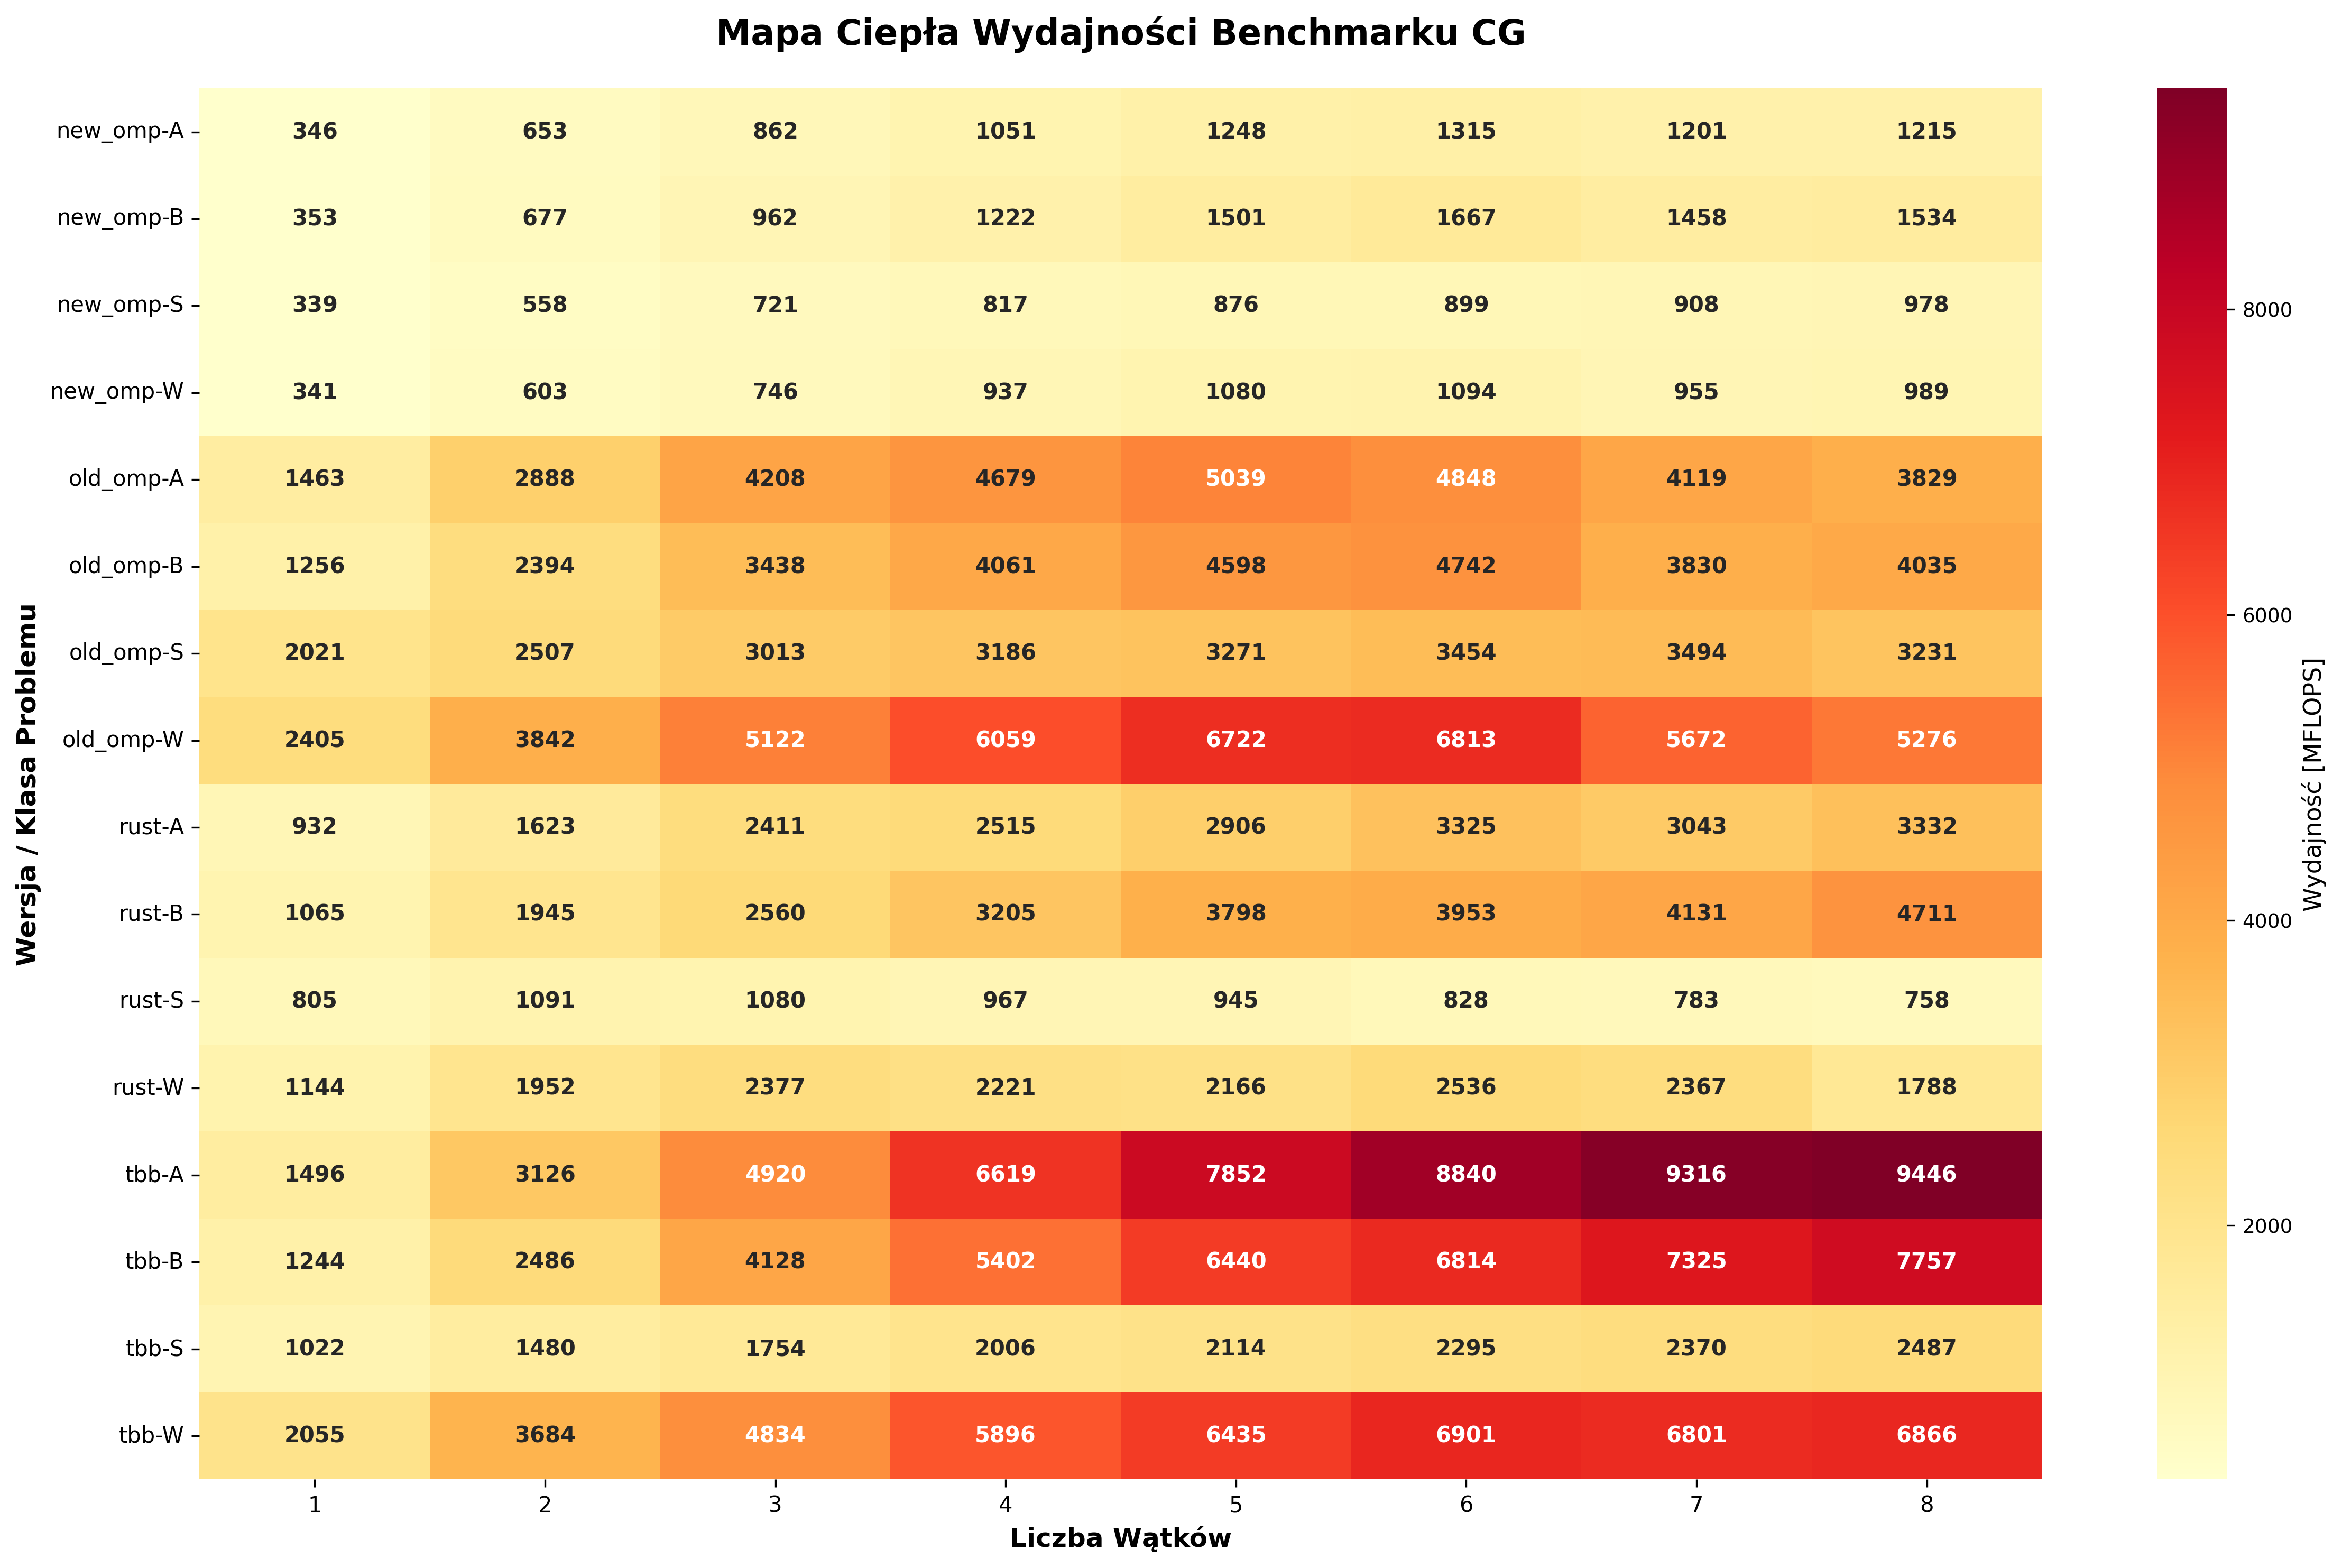
\includegraphics[width=\textwidth]{analiza/images/parallel/cg/x86/cg_mapa_ciepla_wydajnosci.png}
    \caption{Mapa ciepła wydajności benchmarku CG dla klas S, W, A, B względem liczby użytych wątków na platformie ARM64}
    \label{cg_heatmap_wydajnosci_x86_64}
\end{figure}
Mapa ciepła - rysunek \ref{cg_heatmap_wydajnosci_x86_64} wydajności benchmarku CG dostarcza komplementarnego widoku na zachowanie wszystkich implementacji. Intensywność koloru odpowiada wydajności obliczeniowej wyrażonej w MFLOPS, co pozwala na szybką identyfikację obszarów optymalnej wydajności. Najwyższe wartości (reprezentowane ciemnoczerwonymi odcieniami) koncentrują się w obszarze implementacji TBB dla klas A, B i W przy wyższej liczbie wątków. Szczególnie widoczna jest równomierna poprawa wydajności TBB dla klasy A wraz ze wzrostem liczby wątków.

Mapa ciepła potwierdza również wyjątkową charakterystykę klasy S, gdzie najwyższe wartości osiągane są przez implementację old\_omp, a nie TBB jak w pozostałych klasach. Dodatkowo uwydatniony jest gradient wydajności dla implementacji rust i old\_omp w klasach A i W, gdzie wydajność najpierw rośnie, a następnie spada przy wyższych liczbach wątków. wydajności.

\begin{figure}[H]
    \centering
    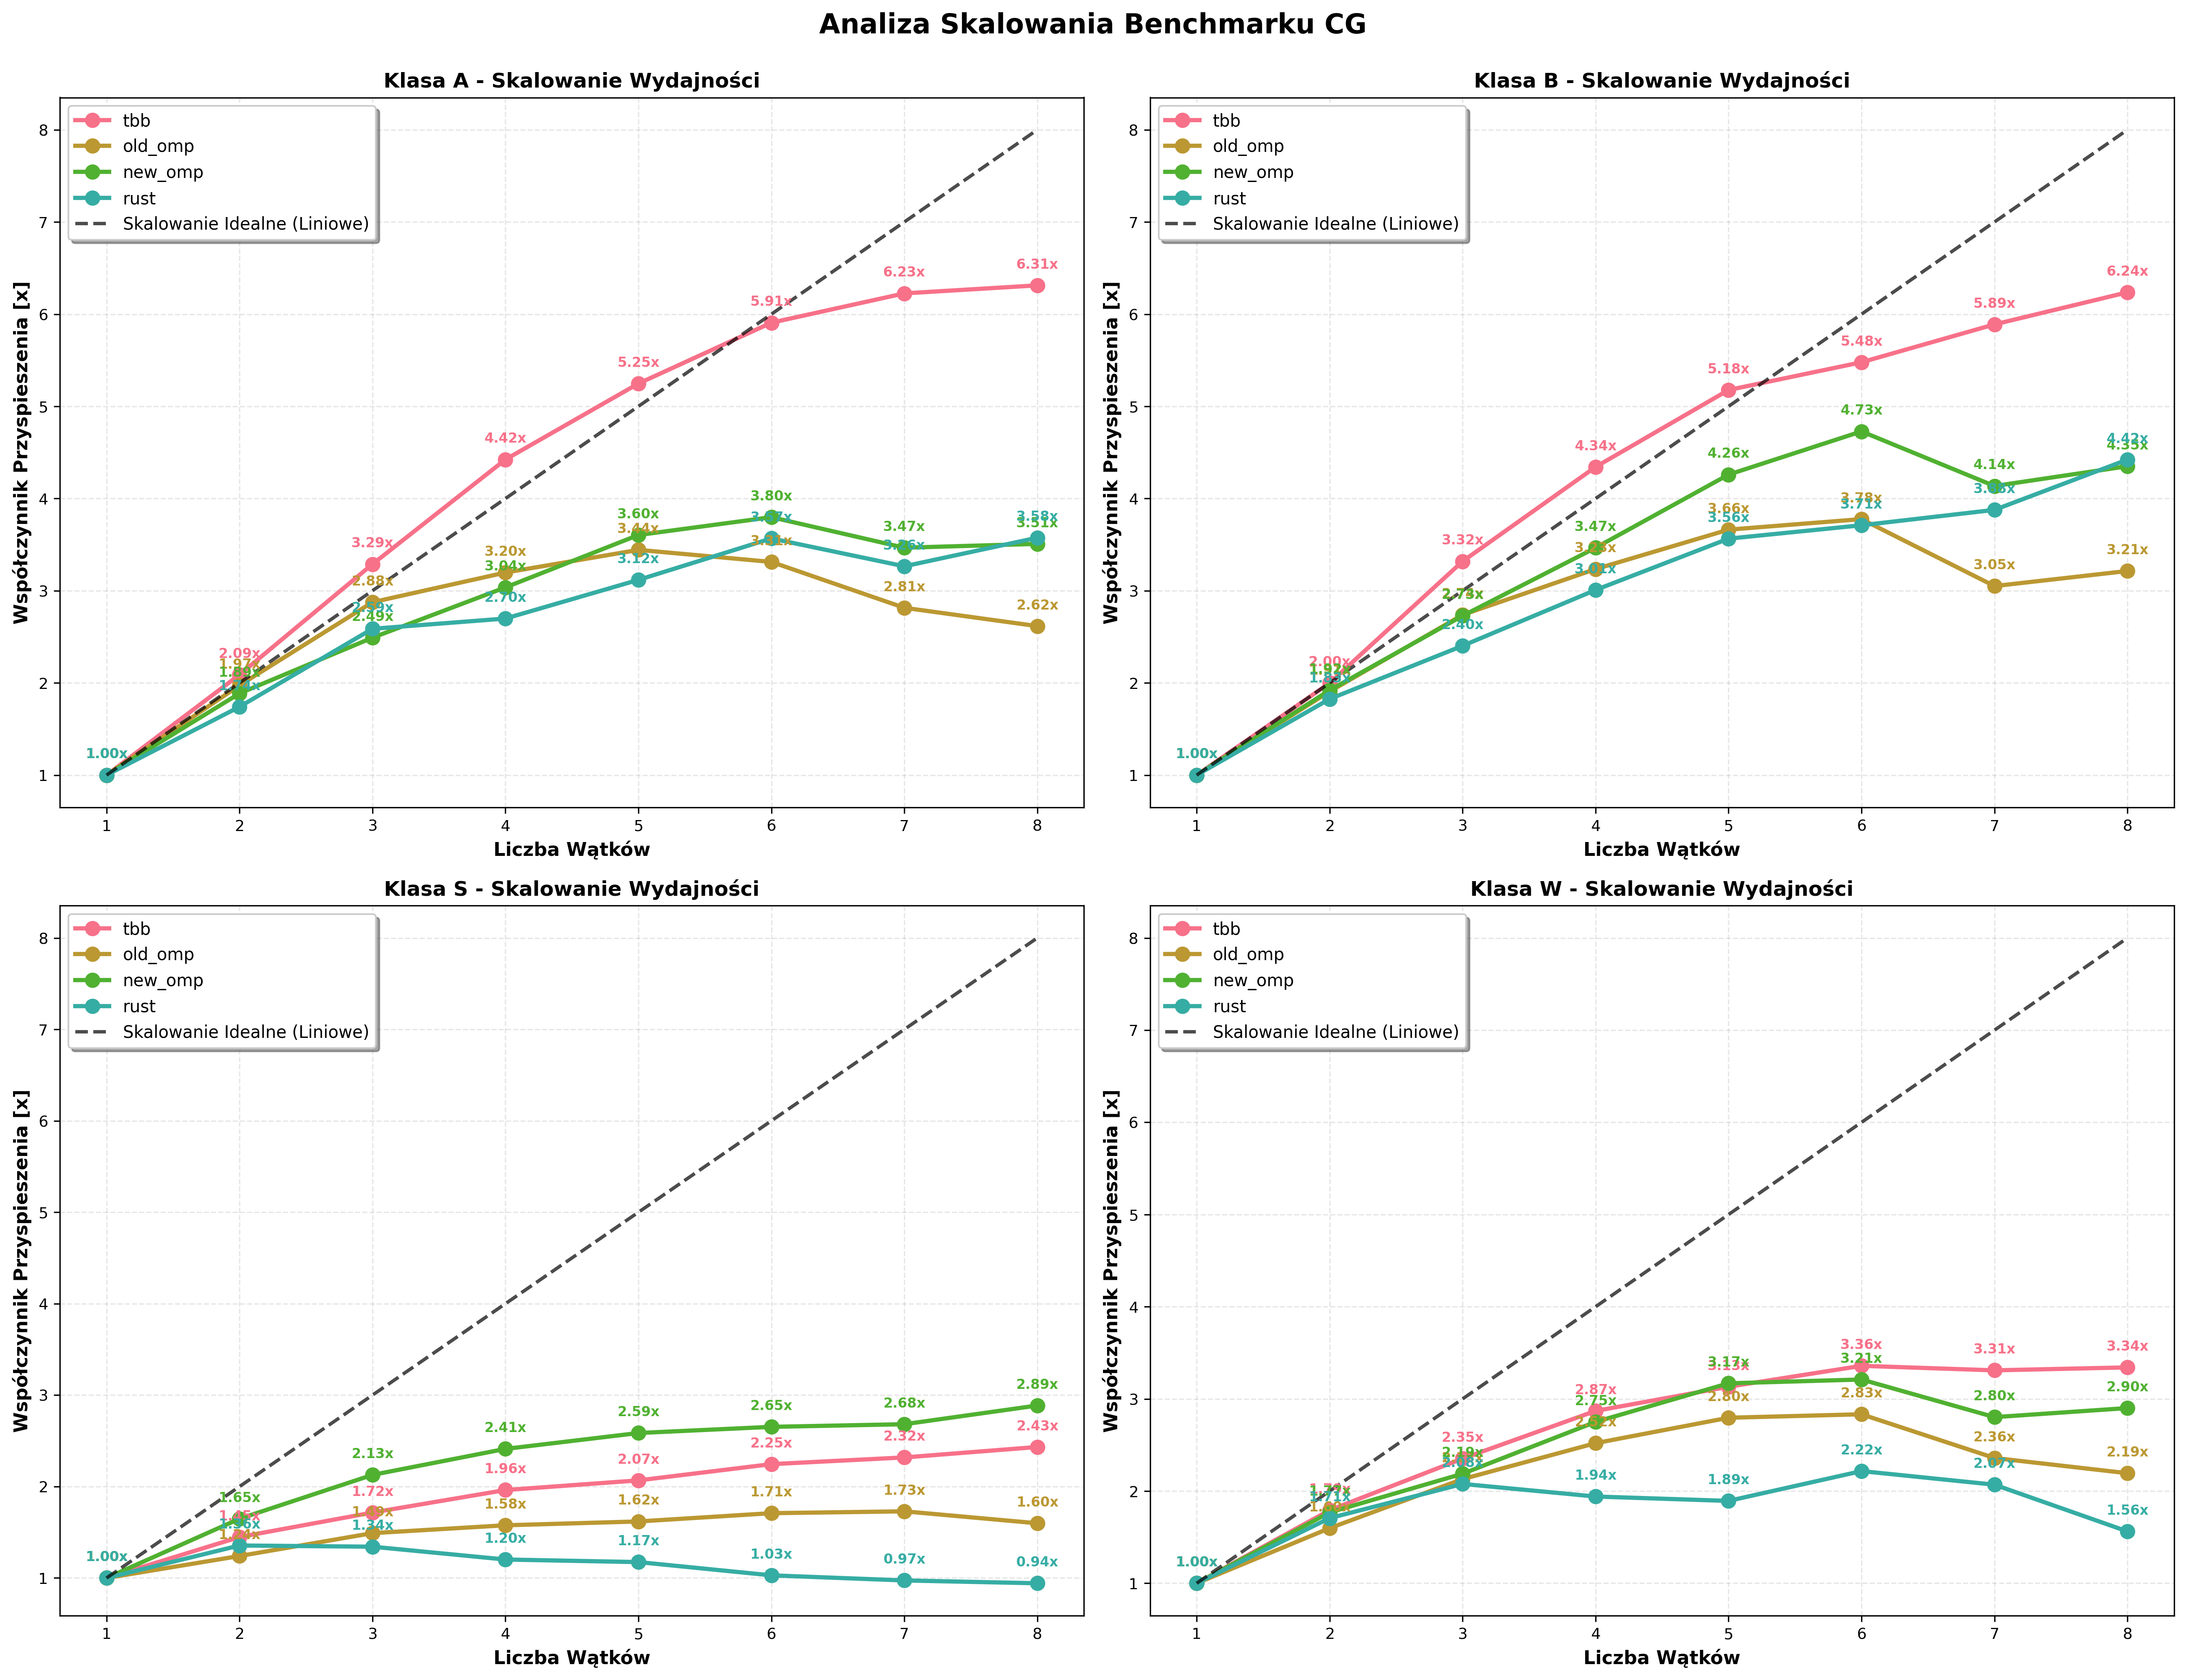
\includegraphics[width=\textwidth]{analiza/images/parallel/cg/x86/cg_analiza_skalowania.png}
    \caption{Analiza skalowania benchmarku CG dla klas S, W, A, B względem liczby użytych wątków na platformie ARM64}
    \label{cg_analiza_skalowania_x86_64}
\end{figure}
Powyższy wykres - rysunek \ref{cg_analiza_skalowania_x86_64} przedstawia skalowanie wydajności benchmarku CG. Skalowanie wyrażone zostało za pomocą współczynnika przyspieszenia względem wykonania jednowątkowego i odniesione do skalowania idealnego (liniowego).
\subsubsection{Porównanie efektywności skalowania implementacji}
Wśród badanych implementacji najlepsze właściwości skalowania wykazuje TBB, szczególnie w klasach A i B, gdzie osiąga przyspieszenie przekraczające 6x przy maksymalnej liczbie wątków. W klasie A zaobserwowano nawet zjawisko superliniowego przyspieszenia (powyżej 6x), co może wynikać z lepszej lokalności pamięci podręcznej.

New\_omp prezentuje umiarkowane, ale stabilne skalowanie. W klasie B osiąga maksymalnie 4,7x przy 6 wątkach, a w innych klasach - niższe wartości. Jej charakterystyczną cechą jest brak gwałtownych spadków wydajności przy rosnącej liczbie wątków.

Rust wykazuje silne zróżnicowanie: w klasach A i B uzyskuje do 3,5x przy 8 wątkach, ale w klasie S dochodzi do degradacji - przyspieszenie spada poniżej 1.0, co świadczy o poważnych problemach z równoległością przy małych problemach.

Old\_omp wypada najsłabiej. Dla większości klas przyspieszenie przestaje rosnąć po 3-4 wątkach. W klasie A przy 8 wątkach osiąga tylko 2,5x, co sugeruje nieefektywność synchronizacji.

\subsubsection{Wpływ klasy problemu}
Najlepsze skalowanie występuje w klasach A i B, gdzie implementacja TBB osiąga przyspieszenia ponad 6x. Klasy te są najbardziej podatne na równoległość.

Klasa S wypada najgorzej - żadna implementacja nie przekracza 3x przyspieszenia, co sugeruje ograniczenia wynikające z wysokiego stosunku komunikacji do obliczeń.

Klasa W wykazuje umiarkowane skalowanie, do ok. 3,5x, przy czym do 3-4 wątków wydajność implementacji jest podobna, po czym zaczynają się różnić.
%------------------------------
%------------------------------
\subsection{Wyniki profilowania wydajności - platforma ARM64}
\begin{figure}[H]
    \centering
    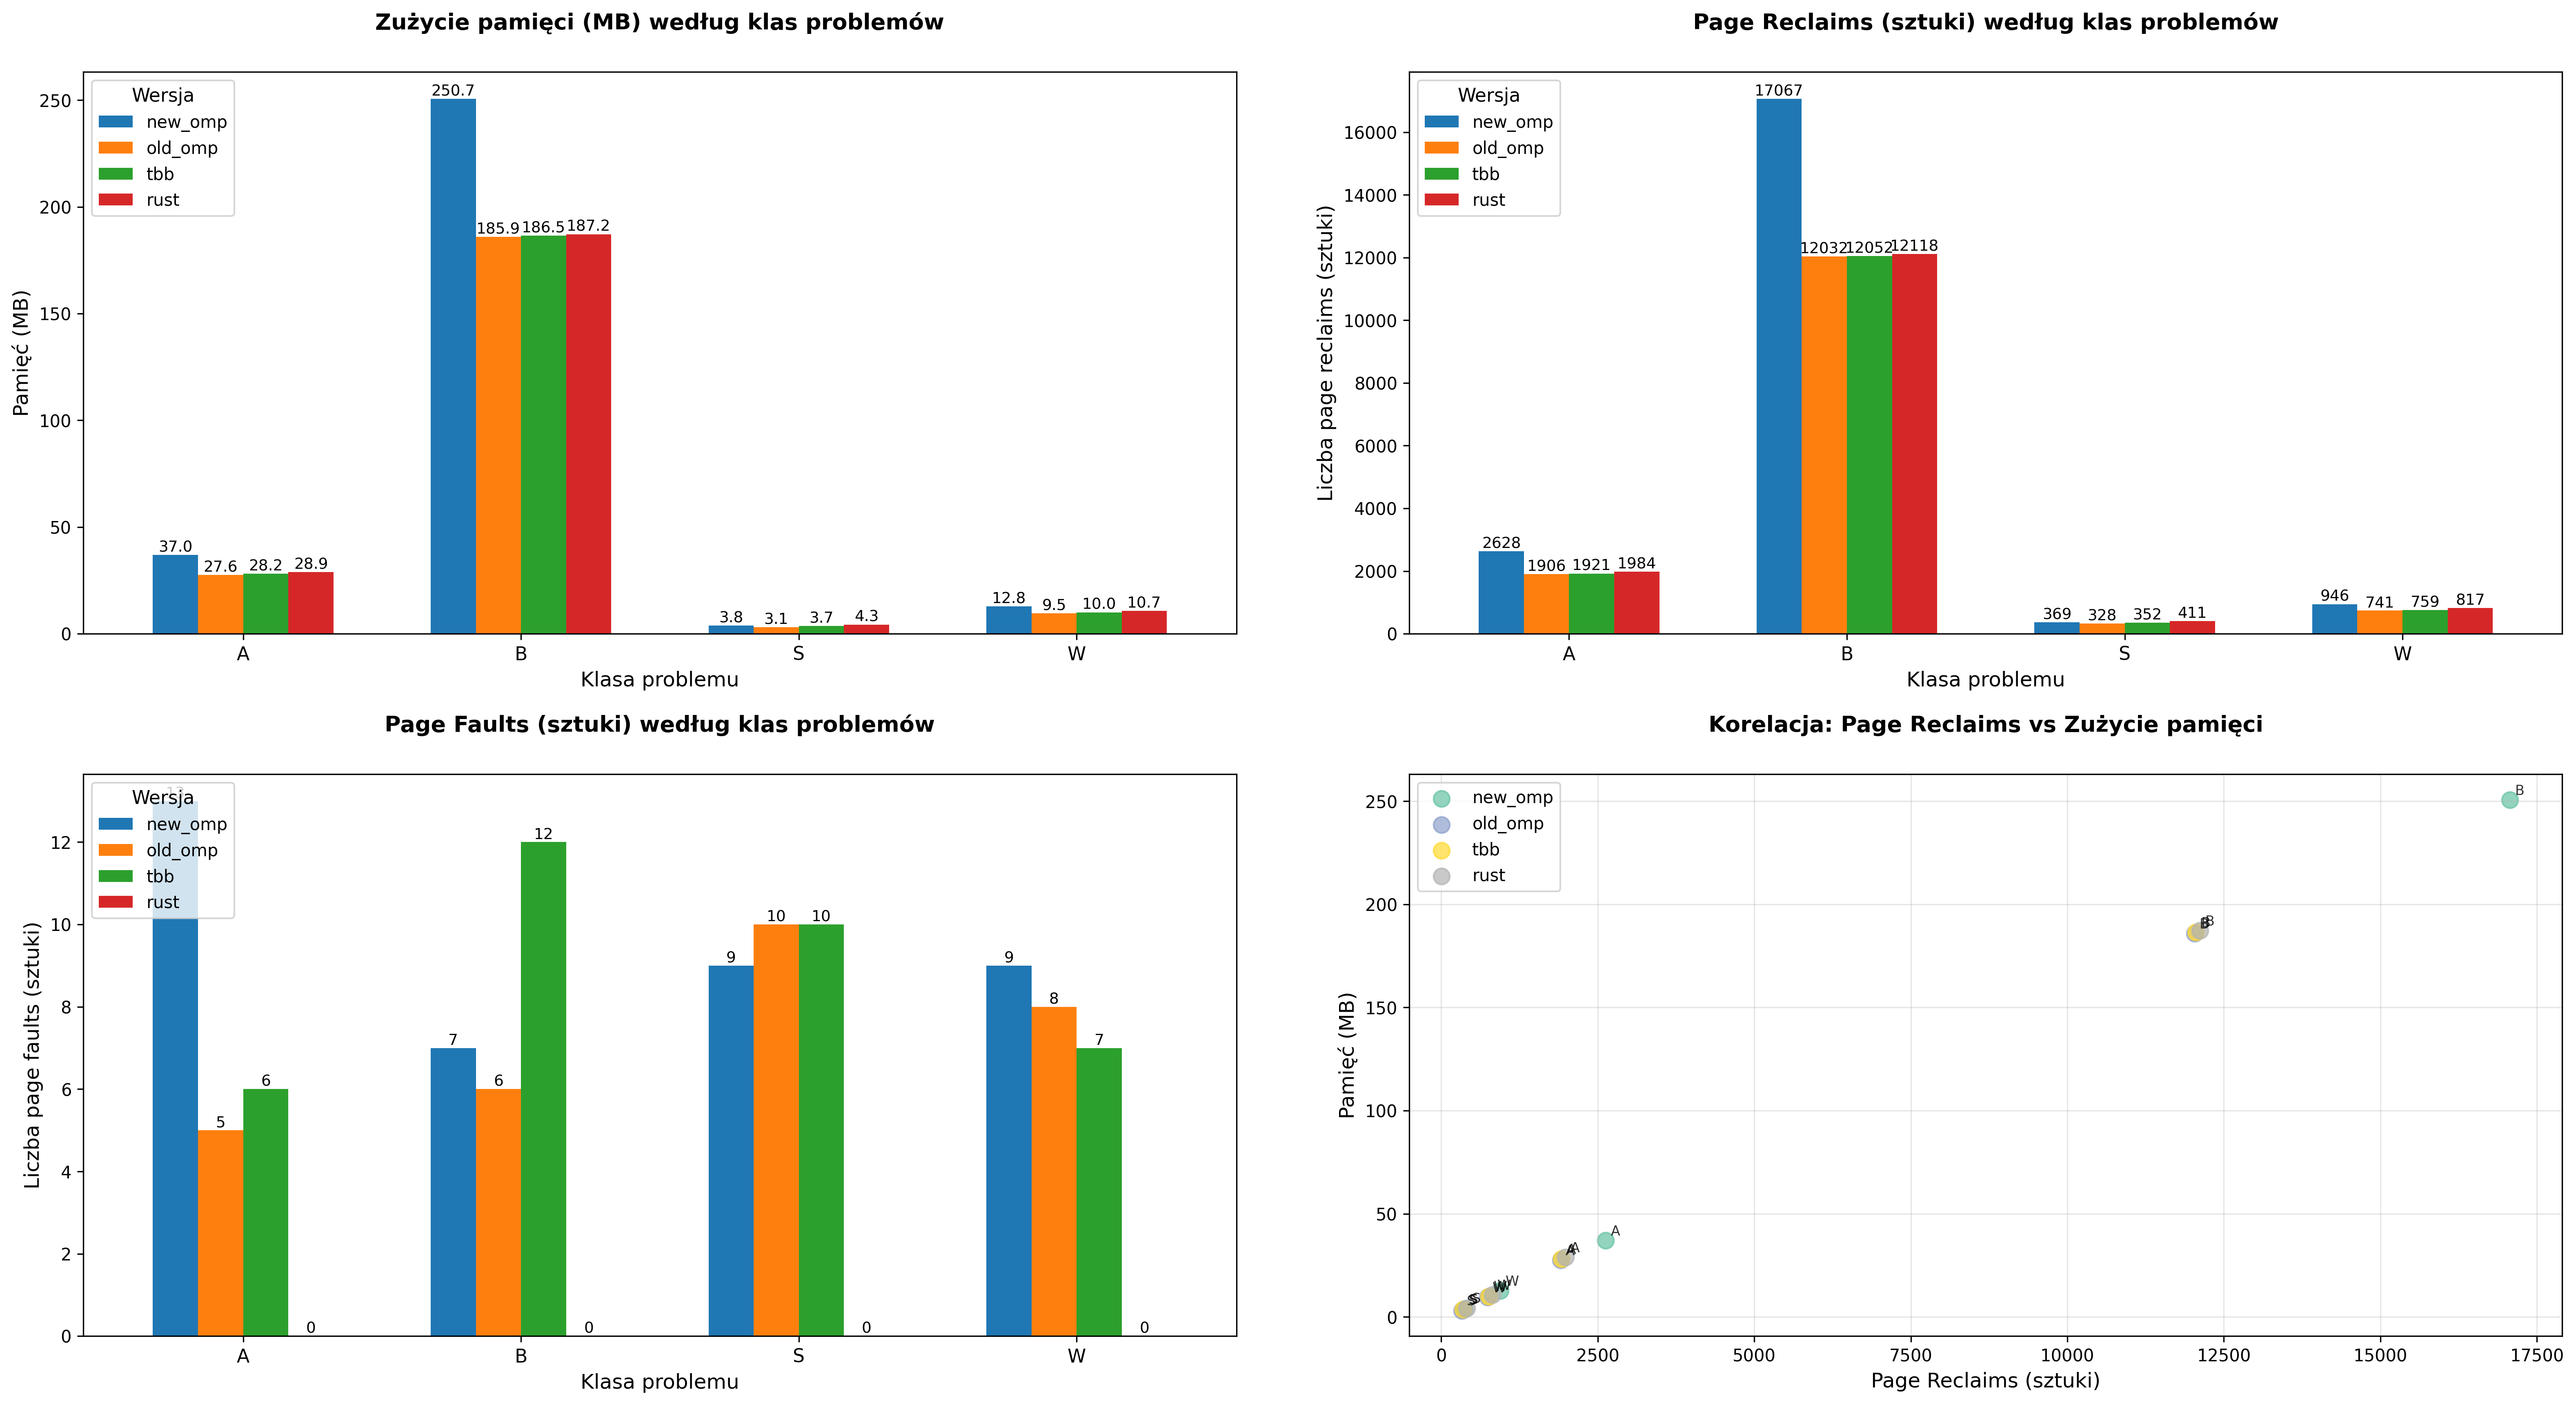
\includegraphics[width=\textwidth]{analiza/images/parallel/cg/arm/chart_01_memory_comparison.png}
    \caption{Profilowanie wydajności benchmarku CG dla klas S, W, A, B względem liczby użytych wątków na platformie ARM64}
    \label{cg_porownanie_zuzycia_pamieci}
\end{figure}

\subsubsection{Zużycie pamięci (MB)}
Na pierwszym wykresie - rysunek \ref{cg_porownanie_zuzycia_pamieci} (lewy górny róg) przedstawiono zużycie pamięci operacyjnej (w MB) dla czterech wersji implementacji algorytmu:
\begin{itemize}
    \item W klasie problemu B występuje najwyższe zużycie pamięci we wszystkich wersjach. Szczególnie zauważalny jest wynik dla new\_omp (250,7 MB), który znacząco przekracza wartości dla pozostałych wersji (około 185-187 MB).
    \item W klasie A new\_omp również zużywa najwięcej pamięci (37 MB), natomiast pozostałe wersje wykazują zbliżony i niższy poziom zużycia (około 27-29 MB).
    \item W klasach S i W różnice są mniej wyraźne, jednak nadal new\_omp wykazuje największe zużycie pamięci.
    \item Wersja rust generalnie charakteryzuje się najmniejszym lub jednym z najmniejszych zużyć pamięci w większości klas problemów.
\end{itemize}

\subsubsection{Liczba zwalniania stron pamięci (w sztukach)}
Drugi wykres - rysunek \ref{cg_porownanie_zuzycia_pamieci} (prawy górny róg) ilustruje liczbę zwalniania stron pamięci \eng{page reclaim}, czyli sytuacji, w których system operacyjny odzyskuje strony pamięci.
\begin{itemize}
    \item Najwięcej zwalnianych stron pamięci występuje w klasie B dla wersji new\_omp (17067), co koresponduje z jej wysokim zużyciem pamięci.
    \item W pozostałych wersjach liczba zwolnionych stron w klasie B jest znacznie niższa (około 12000-12100).
    \item W klasie A new\_omp ponownie osiąga najwyższy wynik (2628), przy niższych wartościach pozostałych wersji (około 1900).
    \item W klasach S i W różnice są mniej zauważalne, choć new\_omp nadal wykazuje wyższe wartości.
\end{itemize}

\subsubsection{Odwołania do nieobecnych stron (w sztukach)}

Trzeci wykres - rysunek \ref{cg_porownanie_zuzycia_pamieci} (lewy dolny róg) przedstawia odwołania do nieobecnych stronliczbę \eng{page fault} - czyli sytuacji, w których wymagany fragment pamięci nie znajduje się aktualnie w RAM-ie.
\begin{itemize}
    \item W klasie A new\_omp wykazuje najwyższą liczbę page faults (13), zaś rust nie generuje żadnych błędów.
    \item W klasie B najwięcej błędów generuje TBB (12), podczas gdy rust ponownie nie wykazuje żadnych.
    \item W klasach S i W rust również nie generuje page faults, a inne wersje wykazują umiarkowane wartości (7-10).
    \item Wyniki te sugerują bardzo efektywną gospodarkę pamięciową w wersji rust.
\end{itemize}

\subsubsection{Korelacja: Liczba zwalniania stron pamięci a Zużycie pamięci}
Ostatni wykres - rysunek \ref{cg_porownanie_zuzycia_pamieci} (prawy dolny róg) ilustruje zależność pomiędzy liczbą zwolnionych stron pamięci a zużyciem pamięci.
\begin{itemize}
    \item Widoczna jest silna dodatnia korelacja - im większe zużycie pamięci, tym większa liczba zwolnionych stron pamięci. Najwyraźniejszym punktem odniesienia jest wersja new\_omp dla klasy B, która dominuje pod względem obu metryk.
    \item Punkty reprezentujące wersję rust znajdują się w lewej dolnej części wykresu, wskazując na niskie zużycie pamięci i małą liczbę zwolnionych stron.
\end{itemize}

\begin{figure}[H]
    \centering
    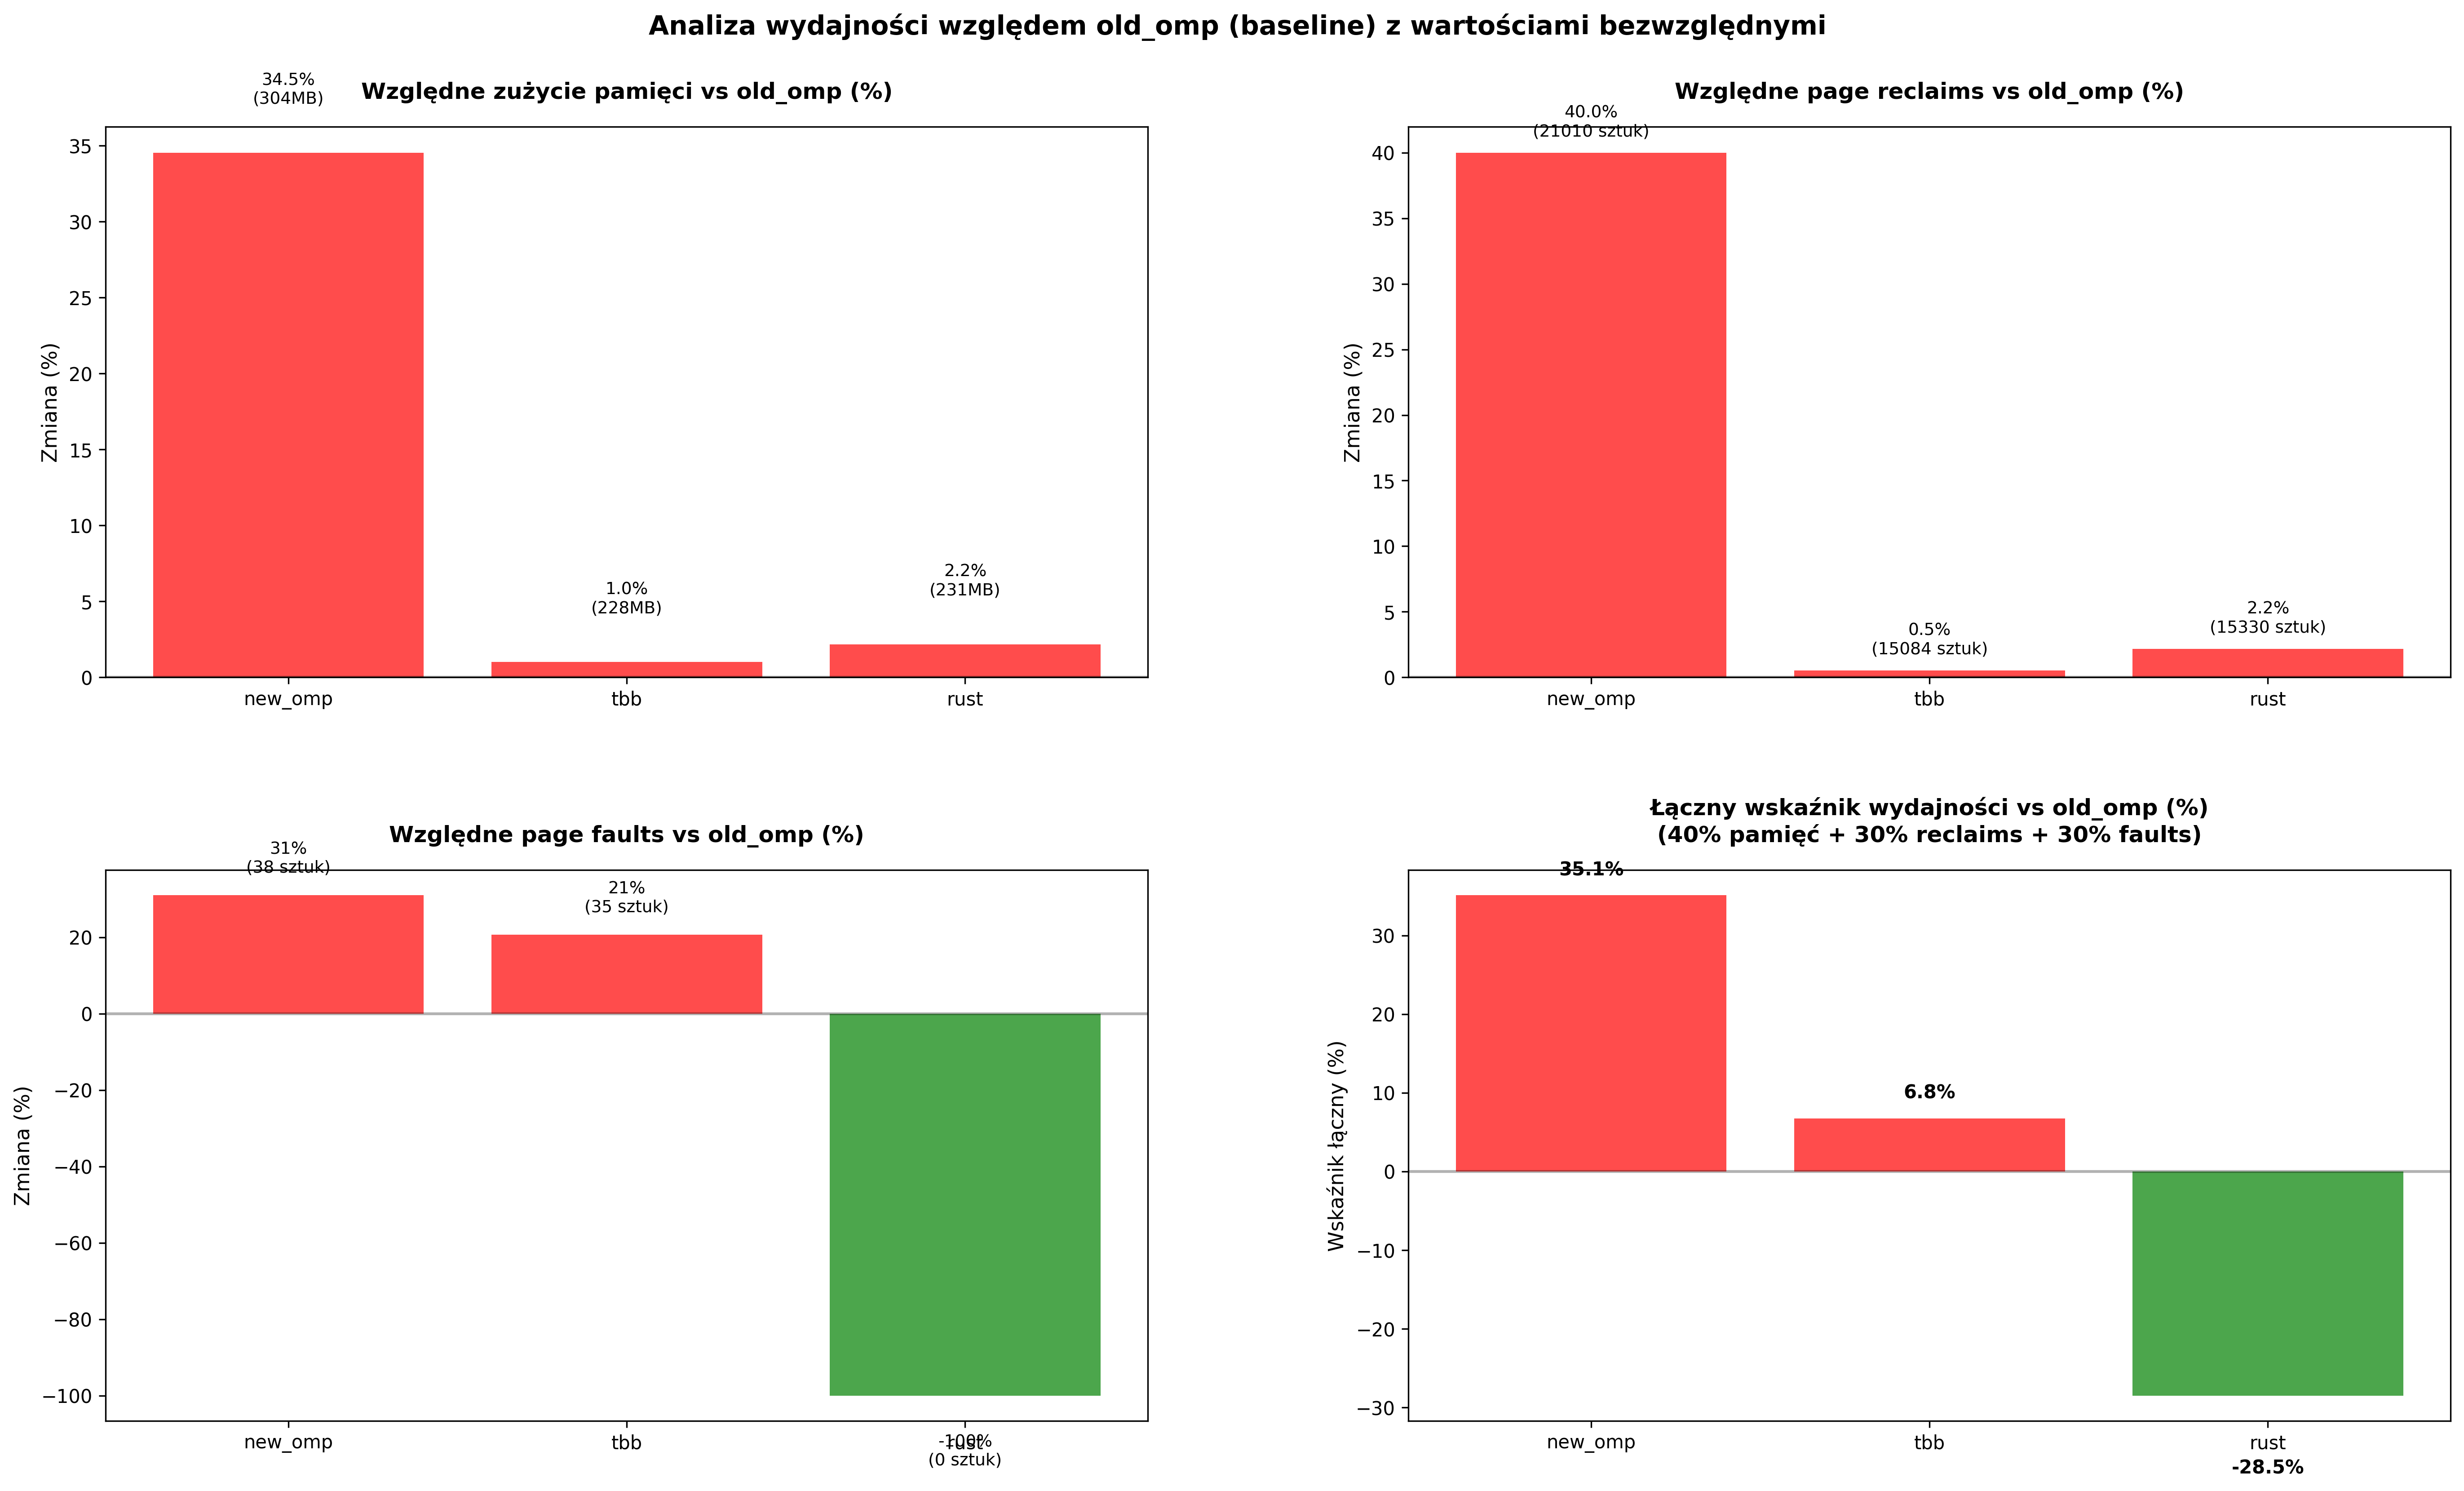
\includegraphics[width=\textwidth]{analiza/images/parallel/cg/arm/chart_05_performance_ratios.png}
    \caption{Analiza wydajności względem old\_omp (punkt odniesienia) z wartościami bezwzględnymi na platformie ARM64}
    \label{cg_analiza_wzgledem_old_omp}
\end{figure}
Na wykresie - rysunek \ref{cg_analiza_wzgledem_old_omp} szczegółowa analiza czterech wykresów przedstawiających względną wydajność trzech wersji implementacji (new\_omp, TBB, rust) względem wersji bazowej old\_omp. Analiza dotyczy zużycia pamięci, liczby zwolnionych stron pamięci, odwołań do nieobecncyh stron oraz skumulowanego wskaźnika efektywności.
\subsubsection{Względne zużycie pamięci na tle old\_omp}
Pierwszy wykres - rysunek \ref{cg_analiza_wzgledem_old_omp} (lewy górny róg) ukazuje procentową zmianę w zużyciu pamięci operacyjnej względem implementacji referencyjnej. Największy wzrost odnotowano dla new\_omp, gdzie zużycie pamięci wzrosło o 34,5\%, co przekłada się na dodatkowe 304 MB. Zmiany dla TBB i rust były marginalne i wyniosły odpowiednio 1,0\% (228 MB) oraz 2,2\% (231 MB), co sugeruje ich większą efektywność w kontekście gospodarowania pamięcią.

\subsubsection{Względne odzyskiwanie stron pamięci na tle old\_omp}
Drugi wykres - rysunek \ref{cg_analiza_wzgledem_old_omp} (prawy górny róg) przedstawia zmiany w liczbie odzyskanych stron pamięci. Implementacja new\_omp wykazała aż 40\% wzrost (21010 stron), co może świadczyć o intensywnym zarządzaniu pamięcią w trakcie wykonywania programu. Dla TBB i rust zmiany były minimalne (odpowiednio 0,5\% i 2,2\%), co może być interpretowane jako korzystny efekt optymalizacji dostępu do pamięci.

\subsubsection{Względne błędy stron na tle old\_omp}
Na trzecim wykresie - rysunek \ref{cg_analiza_wzgledem_old_omp} (lewy dolny róg) obserwujemy względną liczbę błędów stron. new\_omp i TBB odnotowały wzrost liczby błędów stron odpowiednio o 31\% (38 sztuk) i 2\% (35 sztuk), co może wskazywać na mniej wydajne wykorzystanie pamięci w porównaniu z old\_omp. Z kolei rust jako jedyna implementacja odnotowała całkowitą eliminację błędów stron (-100\%, 0 sztuk), co potwierdza wyjątkowo skuteczną kontrolę pamięci operacyjnej - mechanizmy własności oraz pożyczania.

\subsubsection{Łączny wskaźnik wydajności na tle old\_omp}
Na ostatnim wykresie - rysunek \ref{cg_analiza_wzgledem_old_omp} (prawy dolny róg) przedstawiono zagregowany wskaźnik wydajności, będący ważoną sumą trzech poprzednich metryk: 40\% udziału zużycia pamięci, 30\% udziału odzyskiwania stron oraz 30\% udziału błędów stron. Najwyższy wskaźnik (35,1\%) ponownie osiąga new\_omp, co oznacza wyraźnie wyższą konsumpcję zasobów w porównaniu do referencji. TBB wykazuje niewielki wzrost (6,8\%), co czyni go względnie neutralnym względem old\_omp. rust natomiast charakteryzuje się łącznym wskaźnikiem na poziomie -28,5\%, co czyni go najbardziej efektywną implementacją w ujęciu ogólnym.

\begin{figure}[H]
    \centering
    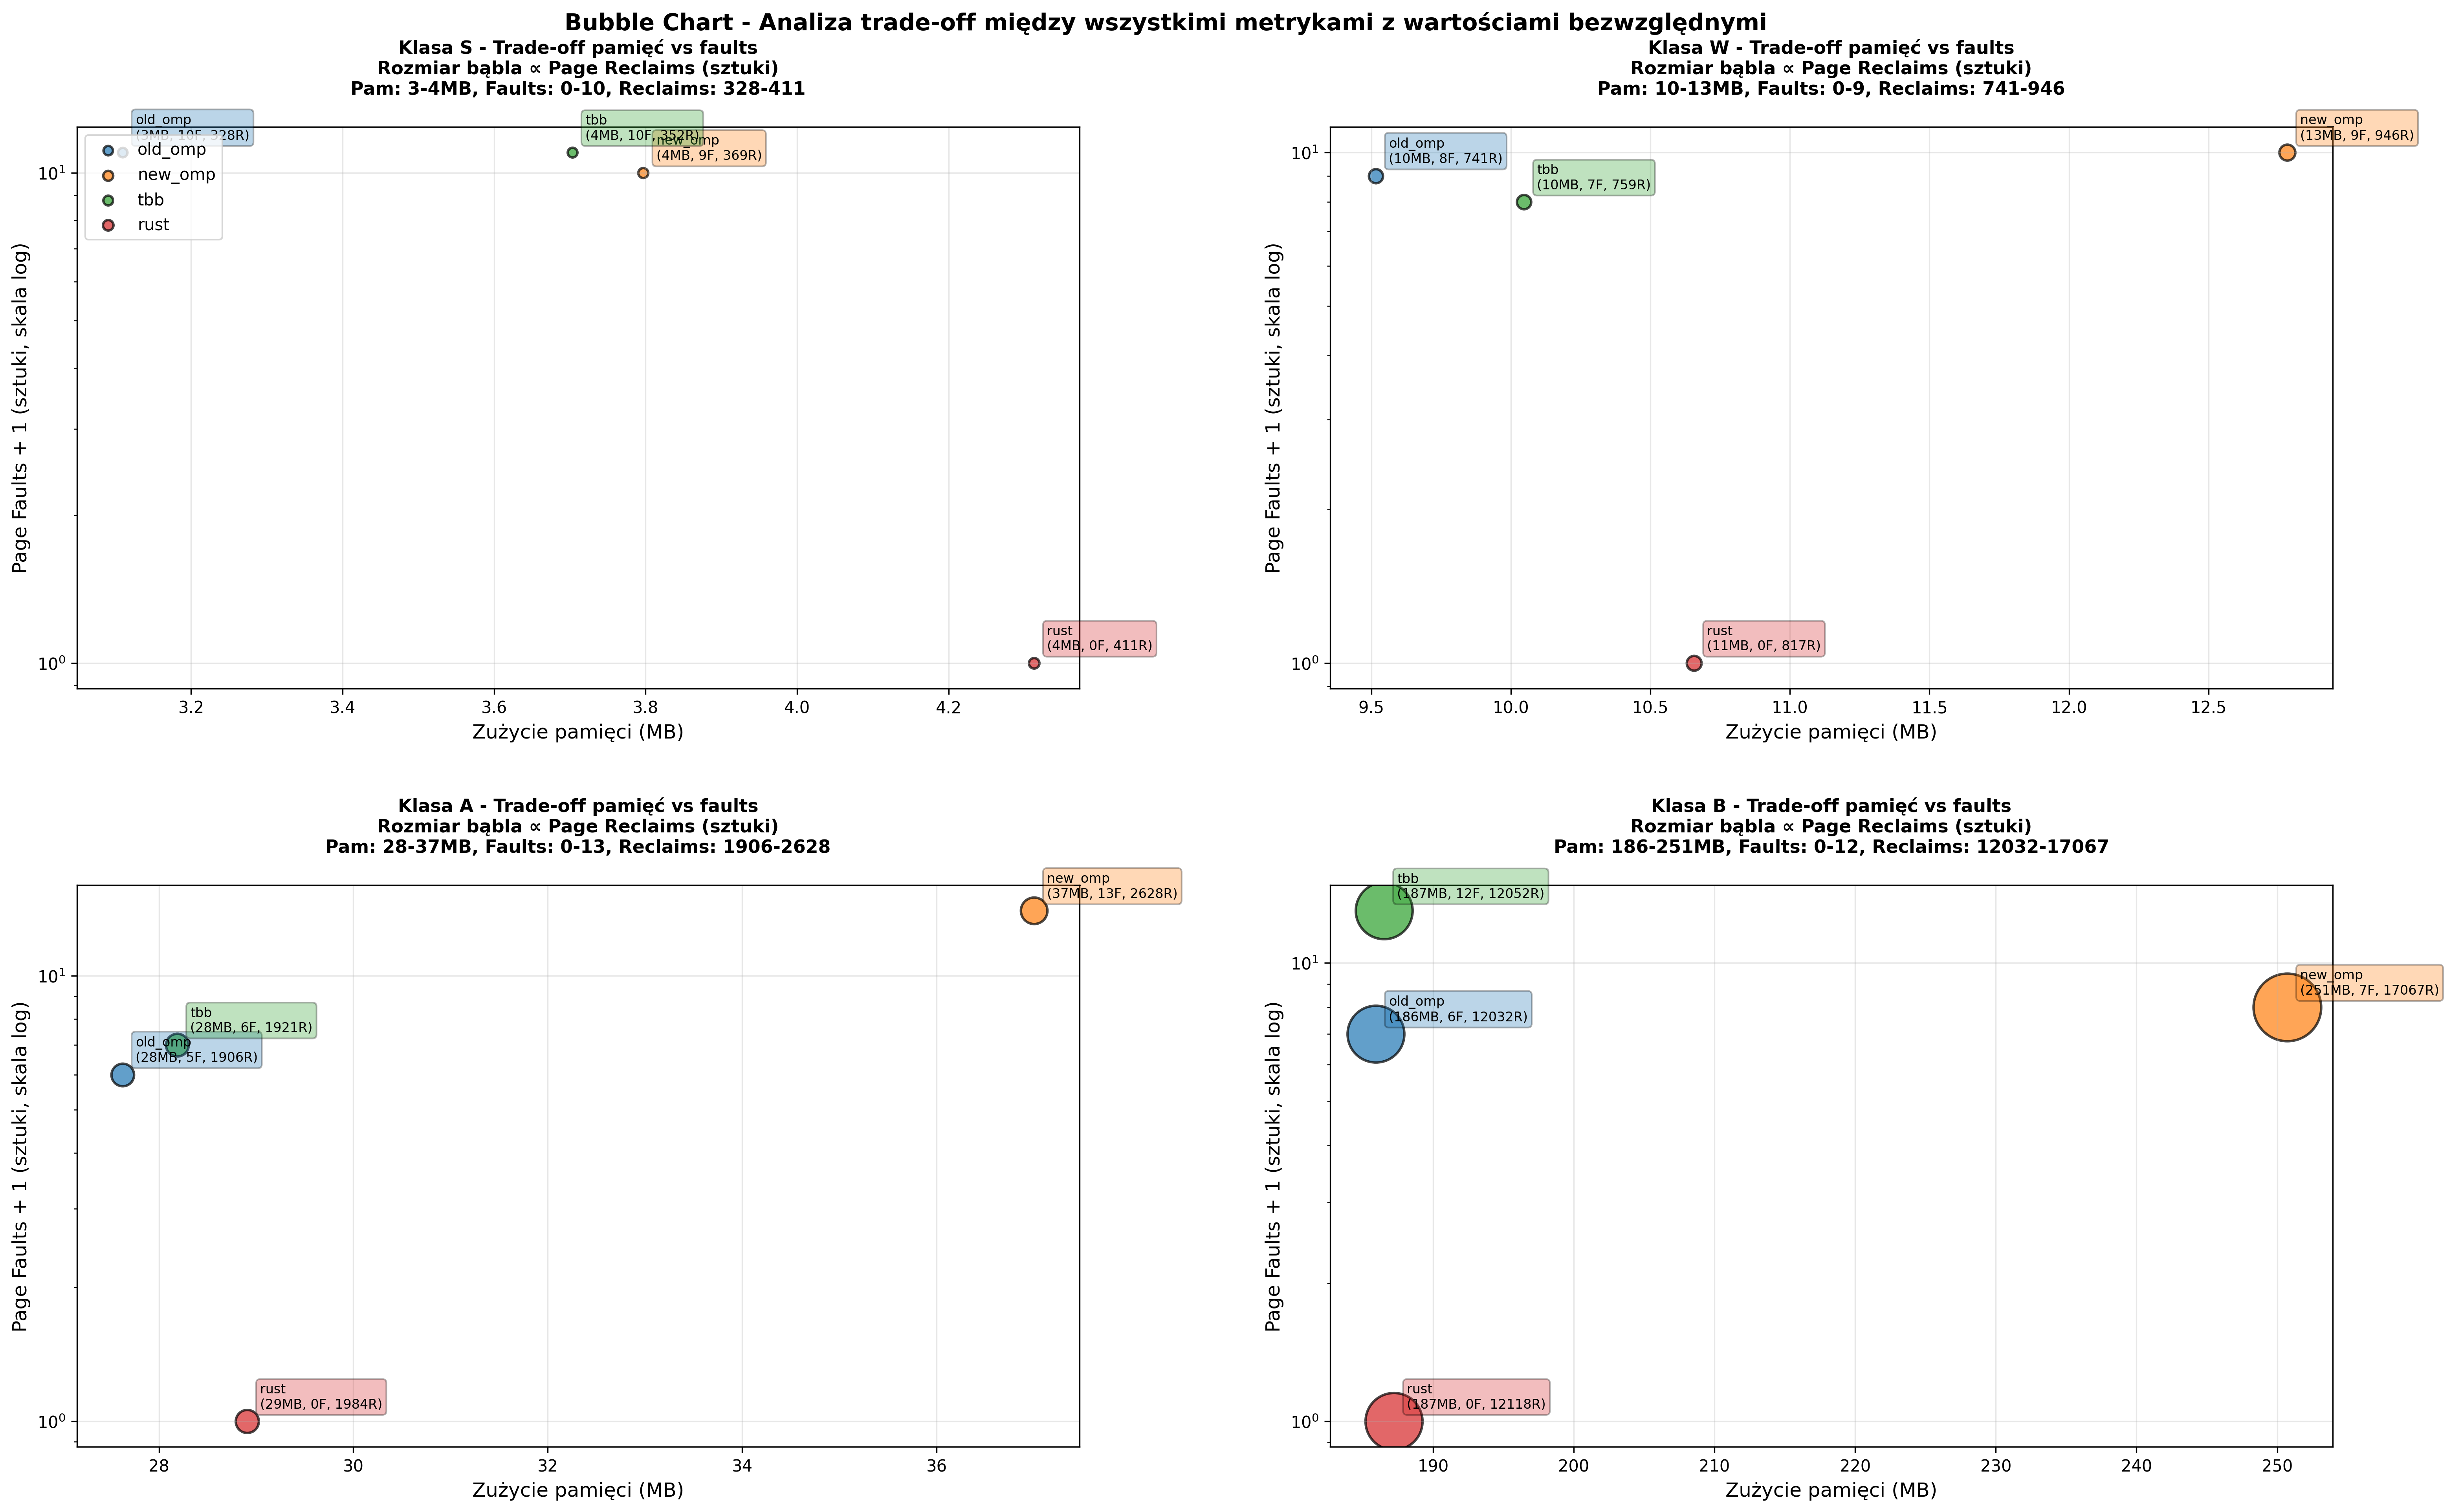
\includegraphics[width=\textwidth]{analiza/images/parallel/cg/arm/chart_06_bubble_chart.png}
    \caption{Kompromisy \eng{trade-off} pomiędzy zużyciem pamięci a błędami stron pamięci, z uwzględnieniem liczby odzyskanych stron jako trzeciej zmiennej reprezentowanej przez rozmiar bąbla na platformie ARM64}
    \label{cg_kompromisy_pamiec_bledy}
\end{figure}

W celu całościowej oceny efektywności pamięciowej badanych implementacji, opracowano wykresy bąbelkowe - rysunek \ref{cg_kompromisy_pamiec_bledy}, które ukazują kompromisy między dwiema kluczowymi metrykami: zużyciem pamięci oraz liczbą błędów stron. Wykresy te wzbogacono o trzeci wymiar - liczbę odzyskanych stron pamięci, która została zakodowana poprzez rozmiar bąbla. Wszystkie wartości przedstawiono w postaci bezwzględnej, przy czym oś Y jest skalowana logarytmicznie w celu lepszego rozróżnienia niewielkich wartości.

Każdy z czterech wykresów odpowiada innej klasie obciążenia pamięciowego (S, W, A, B), przy czym wspólnym celem ich analizy jest uchwycenie relacji pomiędzy wzrostem zużycia pamięci a pogorszeniem lub poprawą stabilności działania (mierzonej błędami stron) oraz intensywnością operacji odzyskiwania stron.

W skali globalnej można zaobserwować, że implementacja rust wielokrotnie wypada korzystnie - cechuje się niskim zużyciem pamięci, zerową liczbą błędów stron w wielu przypadkach oraz stosunkowo niską liczbą zwolnień, co sugeruje wysoką efektywność i dobrą kontrolę nad zarządzaniem pamięcią. Z kolei new\_omp, mimo czasem lepszych wyników obliczeniowych, wykazuje największe zużycie pamięci oraz relatywnie wysoką liczbę błędów stron i odzysków pamięci, co może oznaczać znaczną presję na system zarządzania pamięcią operacyjną.

Implementacja TBB prezentuje wyniki pośrednie, w niektórych przypadkach zbliżone do old\_omp, ale przy lepszym wykorzystaniu zasobów - co czyni ją kompromisowym rozwiązaniem o umiarkowanej efektywności.
-
\subsection{Wyniki profilowania wydajności - platforma x86\_64}
\begin{figure}[H]
    \centering
    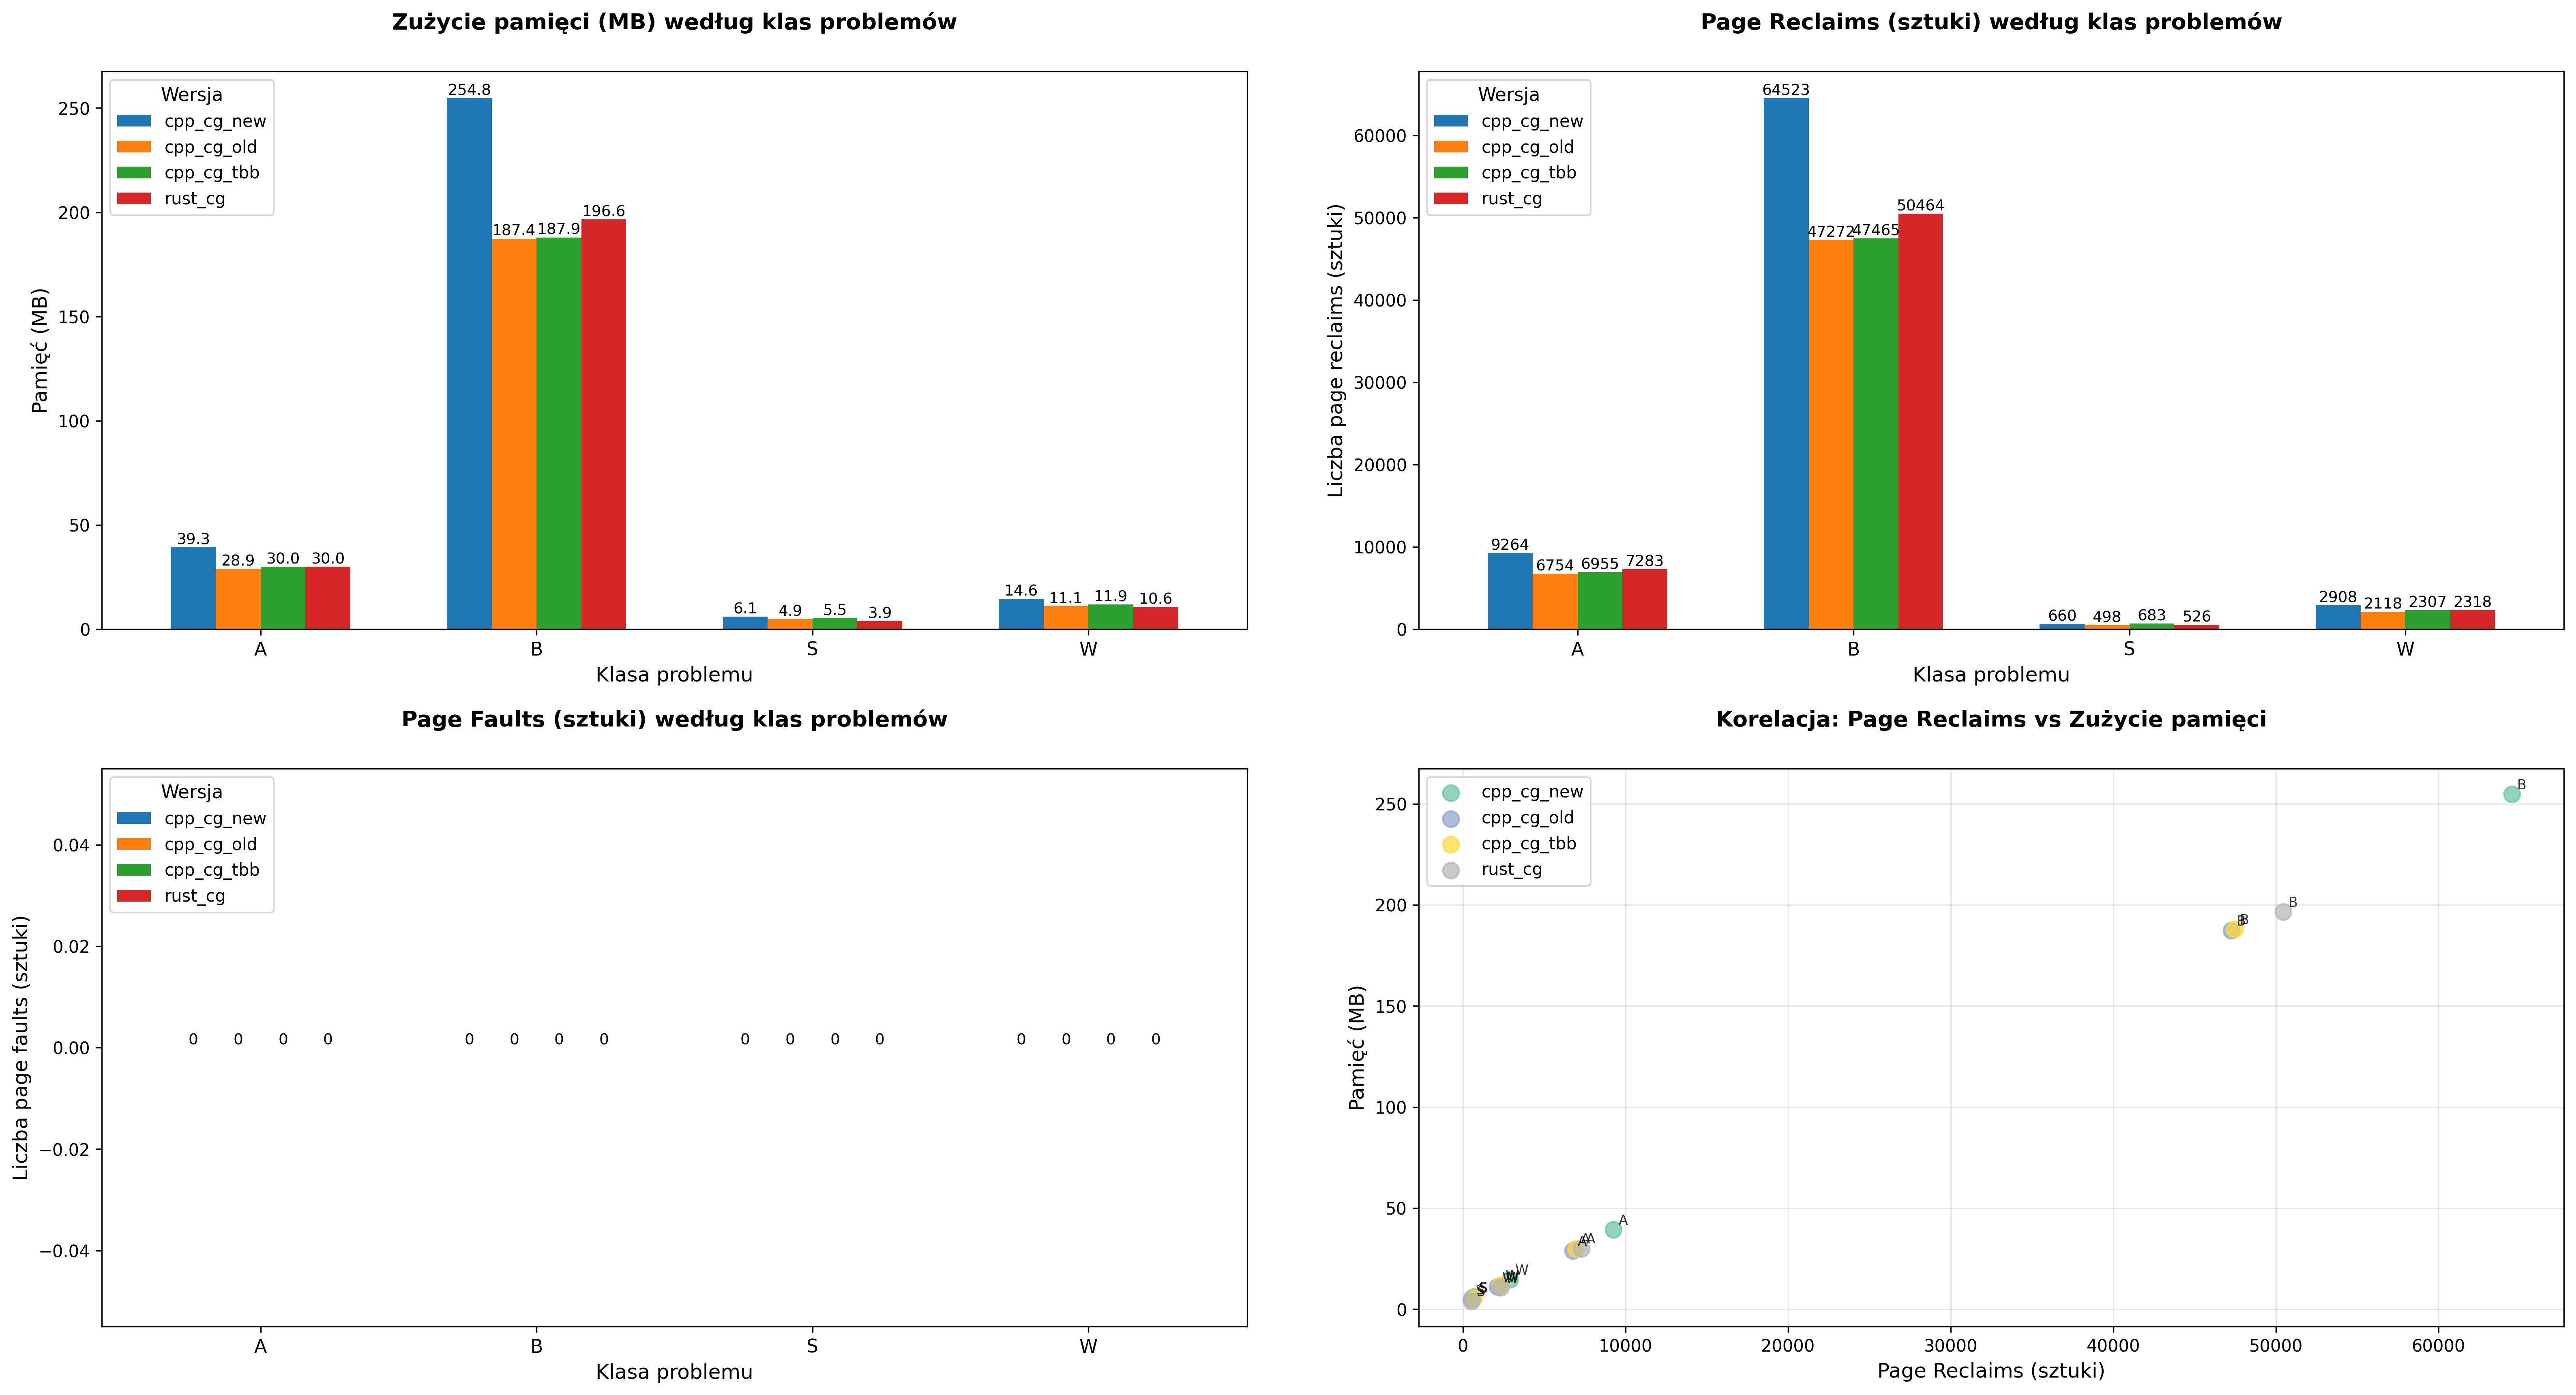
\includegraphics[width=\textwidth]{analiza/images/parallel/cg/x86/chart_01_memory_comparison.png}
    \caption{Profilowanie wydajności benchmarku CG dla klas S, W, A, B względem liczby użytych wątków na platformie x86\_64}
    \label{cg_porownanie_zuzycia_pamieci_x86_64}
\end{figure}
\subsubsection{Zużycie pamięci (MB)}
Z wykresu - rysunek \ref{cg_porownanie_czasow_wykonania_x86_64} zużycia pamięci wynika, że implementacja new\_omp jest zdecydowanie najbardziej pamięciożerna w klasie B, gdzie osiąga wartość 254,8 MB — to istotnie więcej niż pozostałe implementacje, które utrzymują się w zakresie 187-197 MB. Dla pozostałych klas (A, S, W) różnice pomiędzy implementacjami są znikome i mieszczą się w przedziale od 3,9 MB do 39,3 MB.

Zależność zużycia pamięci od klasy problemu jest zgodna z oczekiwaniami: większa klasa (większy problem obliczeniowy) wiąże się z wyższym zużyciem zasobów. Jednak istotna różnica dla new\_omp w klasie B sugeruje potencjalne niedoskonałości w zarządzaniu pamięcią lub większy narzut alokacyjny tej wersji.

\subsubsection{Operacje zwolnień stron (w sztukach)}
Podobnie jak w przypadku zużycia pamięci, new\_omp generuje najwyższe liczby operacji zwolnień stron — w klasie B sięgają one ponad 64 tys. Operacje te wskazują na intensywną aktywność zarządzania pamięcią przez system operacyjny i mogą prowadzić do pogorszenia wydajności w warunkach ograniczonych zasobów. Pozostałe implementacje generują wyraźnie mniej takich operacji (ok. 47-50 tys. dla klasy B).

W klasach A, S i W różnice między implementacjami są mniej znaczące. Warto jednak zwrócić uwagę, że rust we wszystkich klasach cechuje się stosunkowo niskim poziomem zwolnień, co może świadczyć o bardziej efektywnym wykorzystaniu pamięci przez alokator w środowisku Rust.

\subsubsection{Błędy stron (w sztukach)}
Wszystkie implementacje, niezależnie od klasy problemu, wykazują zerowy poziom błędów stron. Taki wynik jest pozytywny i świadczy o prawidłowej alokacji oraz dostępie do pamięci bez potrzeby kosztownego przenoszenia stron pamięci z dysku do RAM-u. To również sugeruje, że żadne z testów nie spowodowały przeciążenia systemu w zakresie dostępnej pamięci fizycznej.

\subsubsection{Korelacja: liczba zwalniania stron pamięci a zużycie pamięci}
Wykres rozrzutu przedstawia silną dodatnią korelację pomiędzy liczbą operacji zwolnień stron a zużyciem pamięci. Punkty odpowiadające klasie B znajdują się wyraźnie w prawym górnym rogu wykresu, potwierdzając, że najbardziej zasobożerna klasa problemu generuje również najwięcej interakcji z systemowym menedżerem pamięci. Punkty dla klas A, S i W rozmieszczone są blisko siebie w lewym dolnym obszarze, co wskazuje na relatywnie stabilne i niskie zużycie pamięci.

\subsubsection{Nota wyjaśniająca}
Ze względu na brak błędów stron nie zamieszczono pozostałych wykresów, które byłyby oparte na tej metryce. Wykresy te nie miałyby sensu, ponieważ brak błędów stron oznacza, że wszystkie operacje pamięciowe były realizowane w ramach dostępnej pamięci fizycznej bez konieczności angażowania mechanizmów swapowania lub przenoszenia stron z dysku.

\subsection{Porównanie pomiędzy platformami}
\subsubsection{Średnia wydajność i współczynnik przyspieszenia}
\begin{figure}[H]
    \centering
    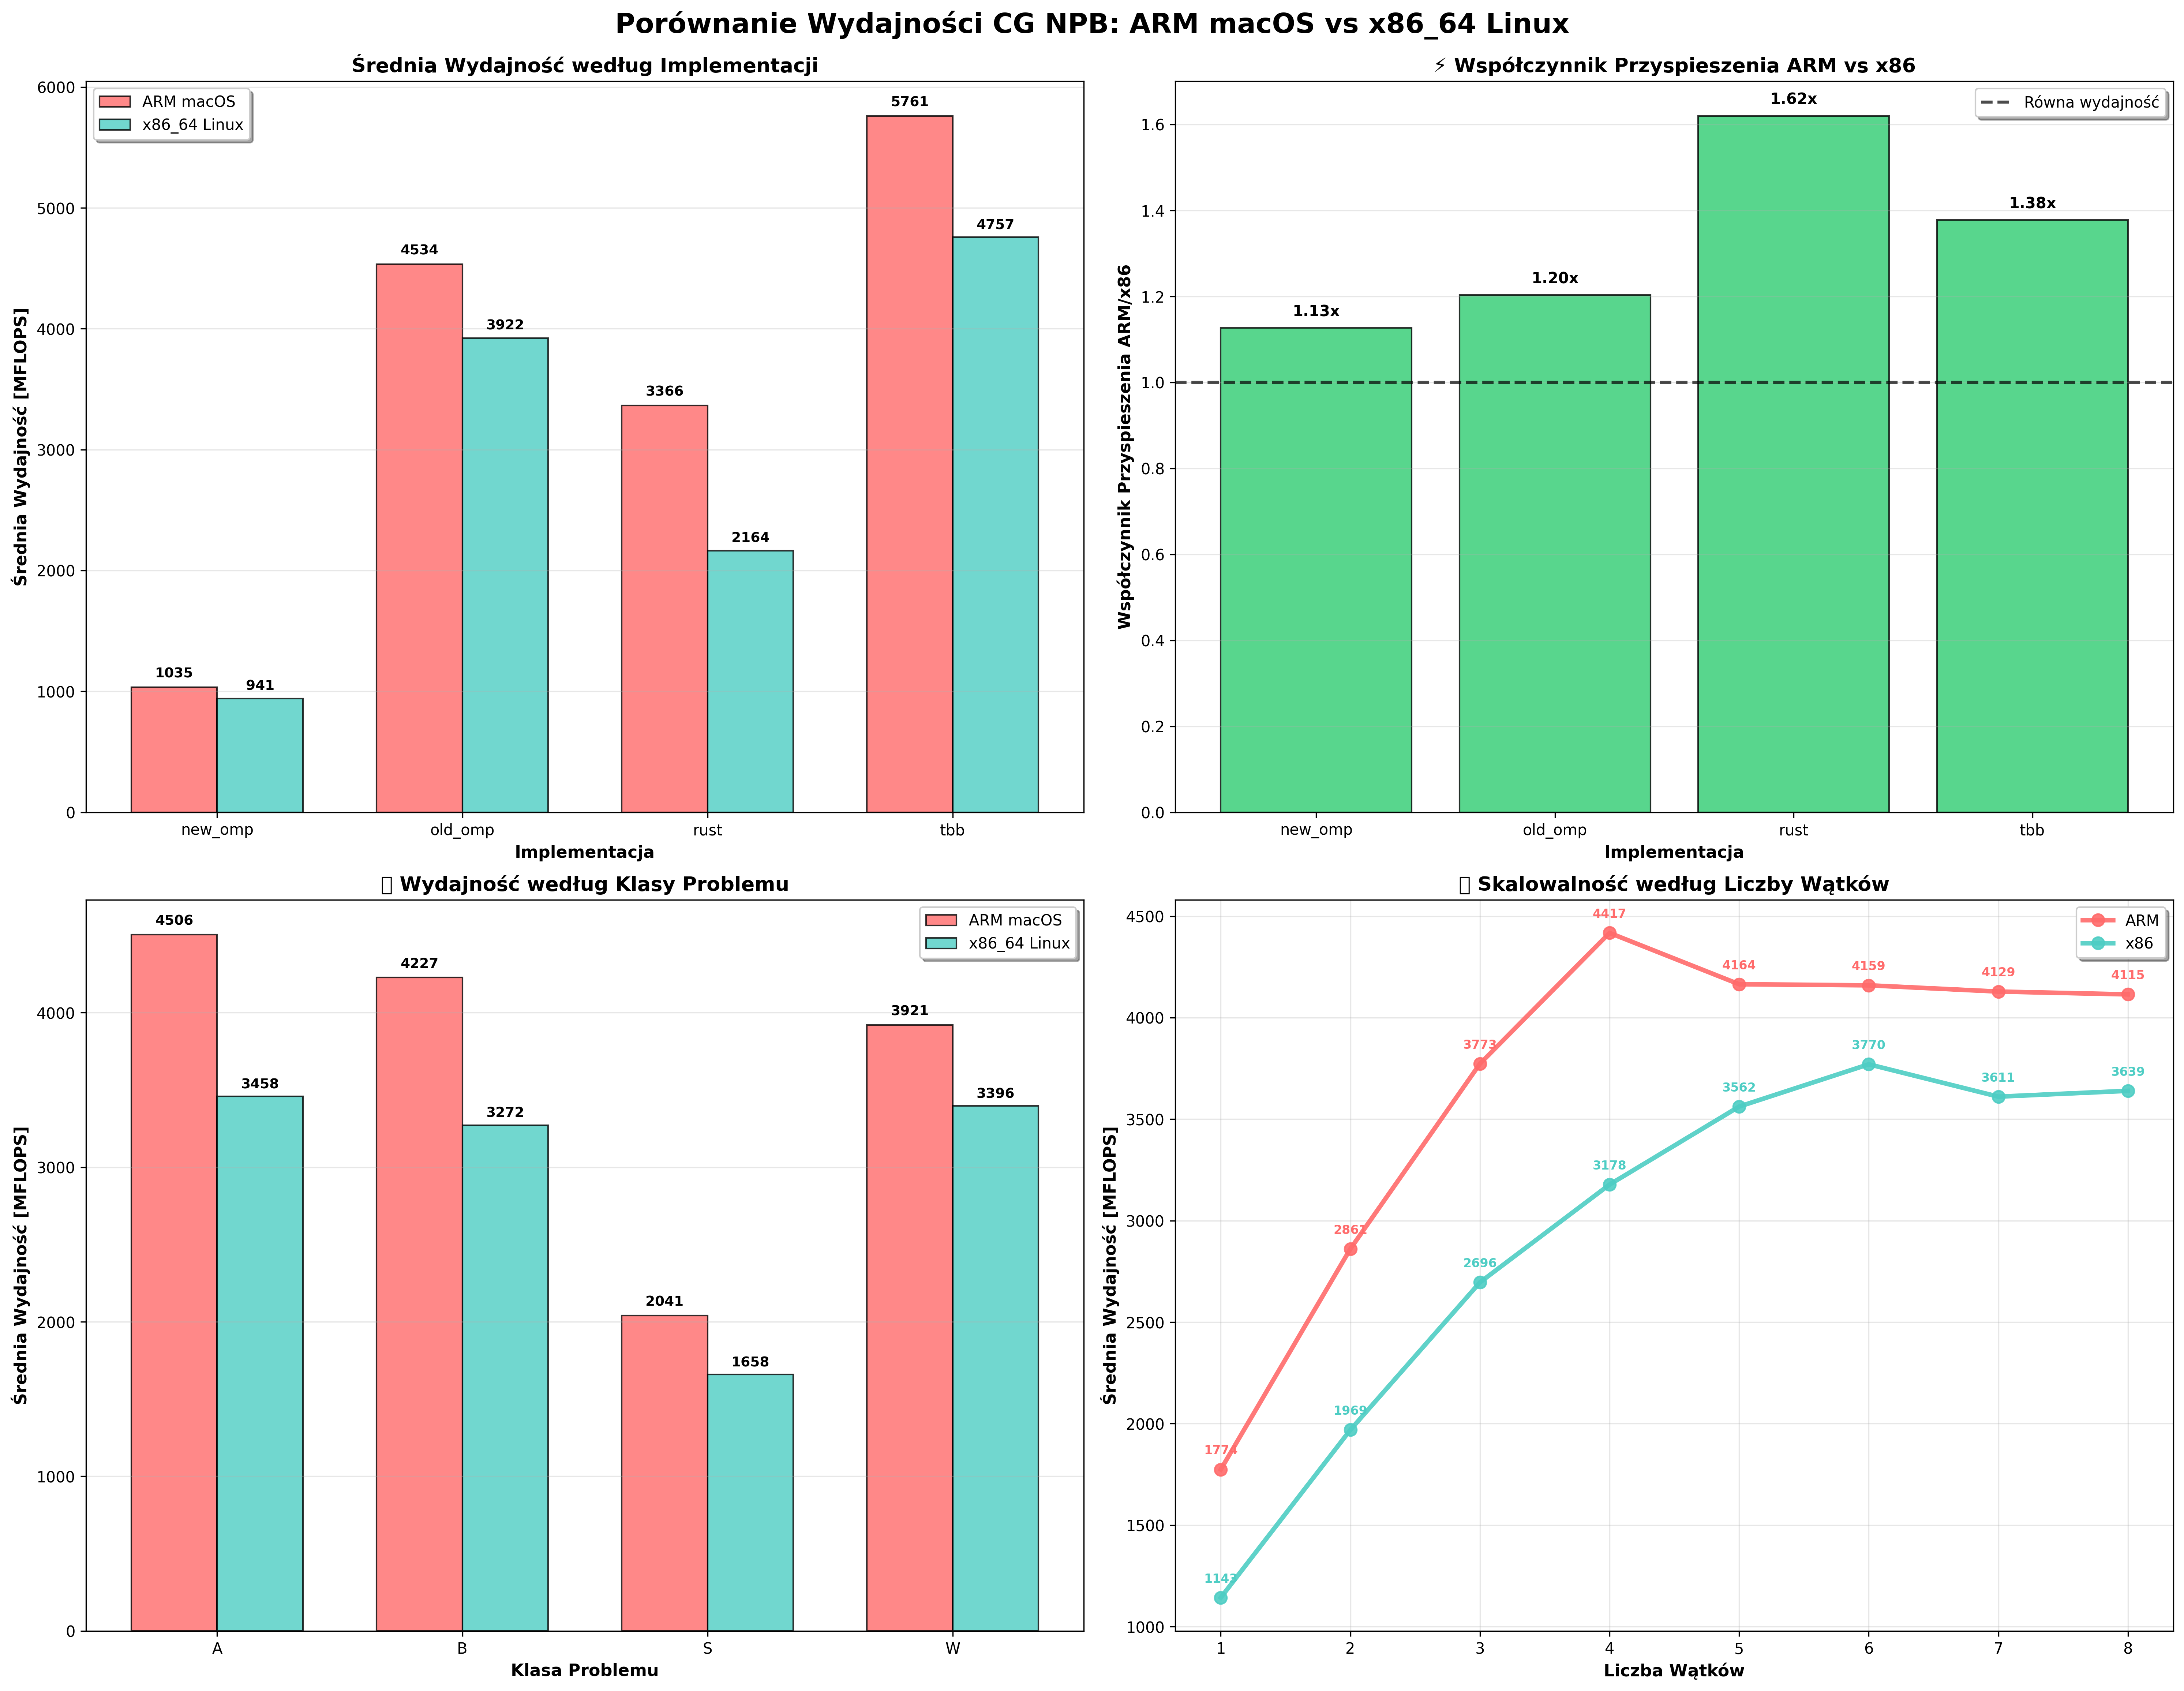
\includegraphics[width=\textwidth]{analiza/images/parallel/cg/compare/cg_porownanie_platform_arm_vs_x86.png}
    \caption{Porównanie średniej wydajności benchmarku CG dla platform ARM64 i x86\_64}
    \label{cg_porownanie_platform_arm_vs_x86}
\end{figure}
Na podstawie wykresów - rysunek \ref{cg_porownanie_platform_arm_vs_x86} uśrednionej wydajności (wyrażonej w MFLOPS) można zaobserwować, że implementacje benchmarku CG uzyskują zróżnicowane rezultaty na obu platformach. Najwyższą wydajność osiąga implementacja tbb na obu architekturach, przy czym wynik dla ARM (5761 MFLOPS) jest wyższy niż dla x86 (4757 MFLOPS). Implementacja rust również wypada lepiej na platformie ARM, uzyskując przewagę nad x86 rzędu 62\% (współczynnik przyspieszenia ARM/x86 = 1.62).

Z kolei old\_omp i new\_omp wykazują mniejsze różnice pomiędzy platformami, jednak nadal na korzyść ARM (współczynnik przyspieszenia odpowiednio 1.20 i 1.13). Pokazuje to, że układy ARM, mimo mniejszej popularności w obliczeniach naukowych, mogą zapewniać porównywalną lub wyższą wydajność w zadaniach równoległych.
\subsubsection{Wydajność względem klasy problemu}
Dla wszystkich klas problemu platforma ARM uzyskuje wyższe wartości MFLOPS w porównaniu do x86, przy czym różnice te są szczególnie widoczne w klasach A i B — odpowiednio 4506 a 3458 oraz 4227 a 3272 MFLOPS. Mniejsze różnice występują w klasach S i W, co może być związane z ograniczoną skalowalnością w mniejszych problemach oraz różnicami w architekturze pamięci podręcznej.
\subsubsection{Skalowanie według liczby wątków}
Analiza wykresu skalowalności pokazuje, że ARM osiąga wyższe wartości MFLOPS w niemal każdej konfiguracji wątkowej. Dla 4 wątków uzyskuje wartość 4417 MFLOPS, przewyższając tym samym x86 (3179 MFLOPS). Mimo że przy wzroście liczby wątków następuje spłaszczenie wykresów dla obu platform, ARM utrzymuje przewagę aż do 8 wątków, co potwierdza dobre skalowanie procesora ARM w tej klasie obliczeń.

\begin{figure}[H]
    \centering
    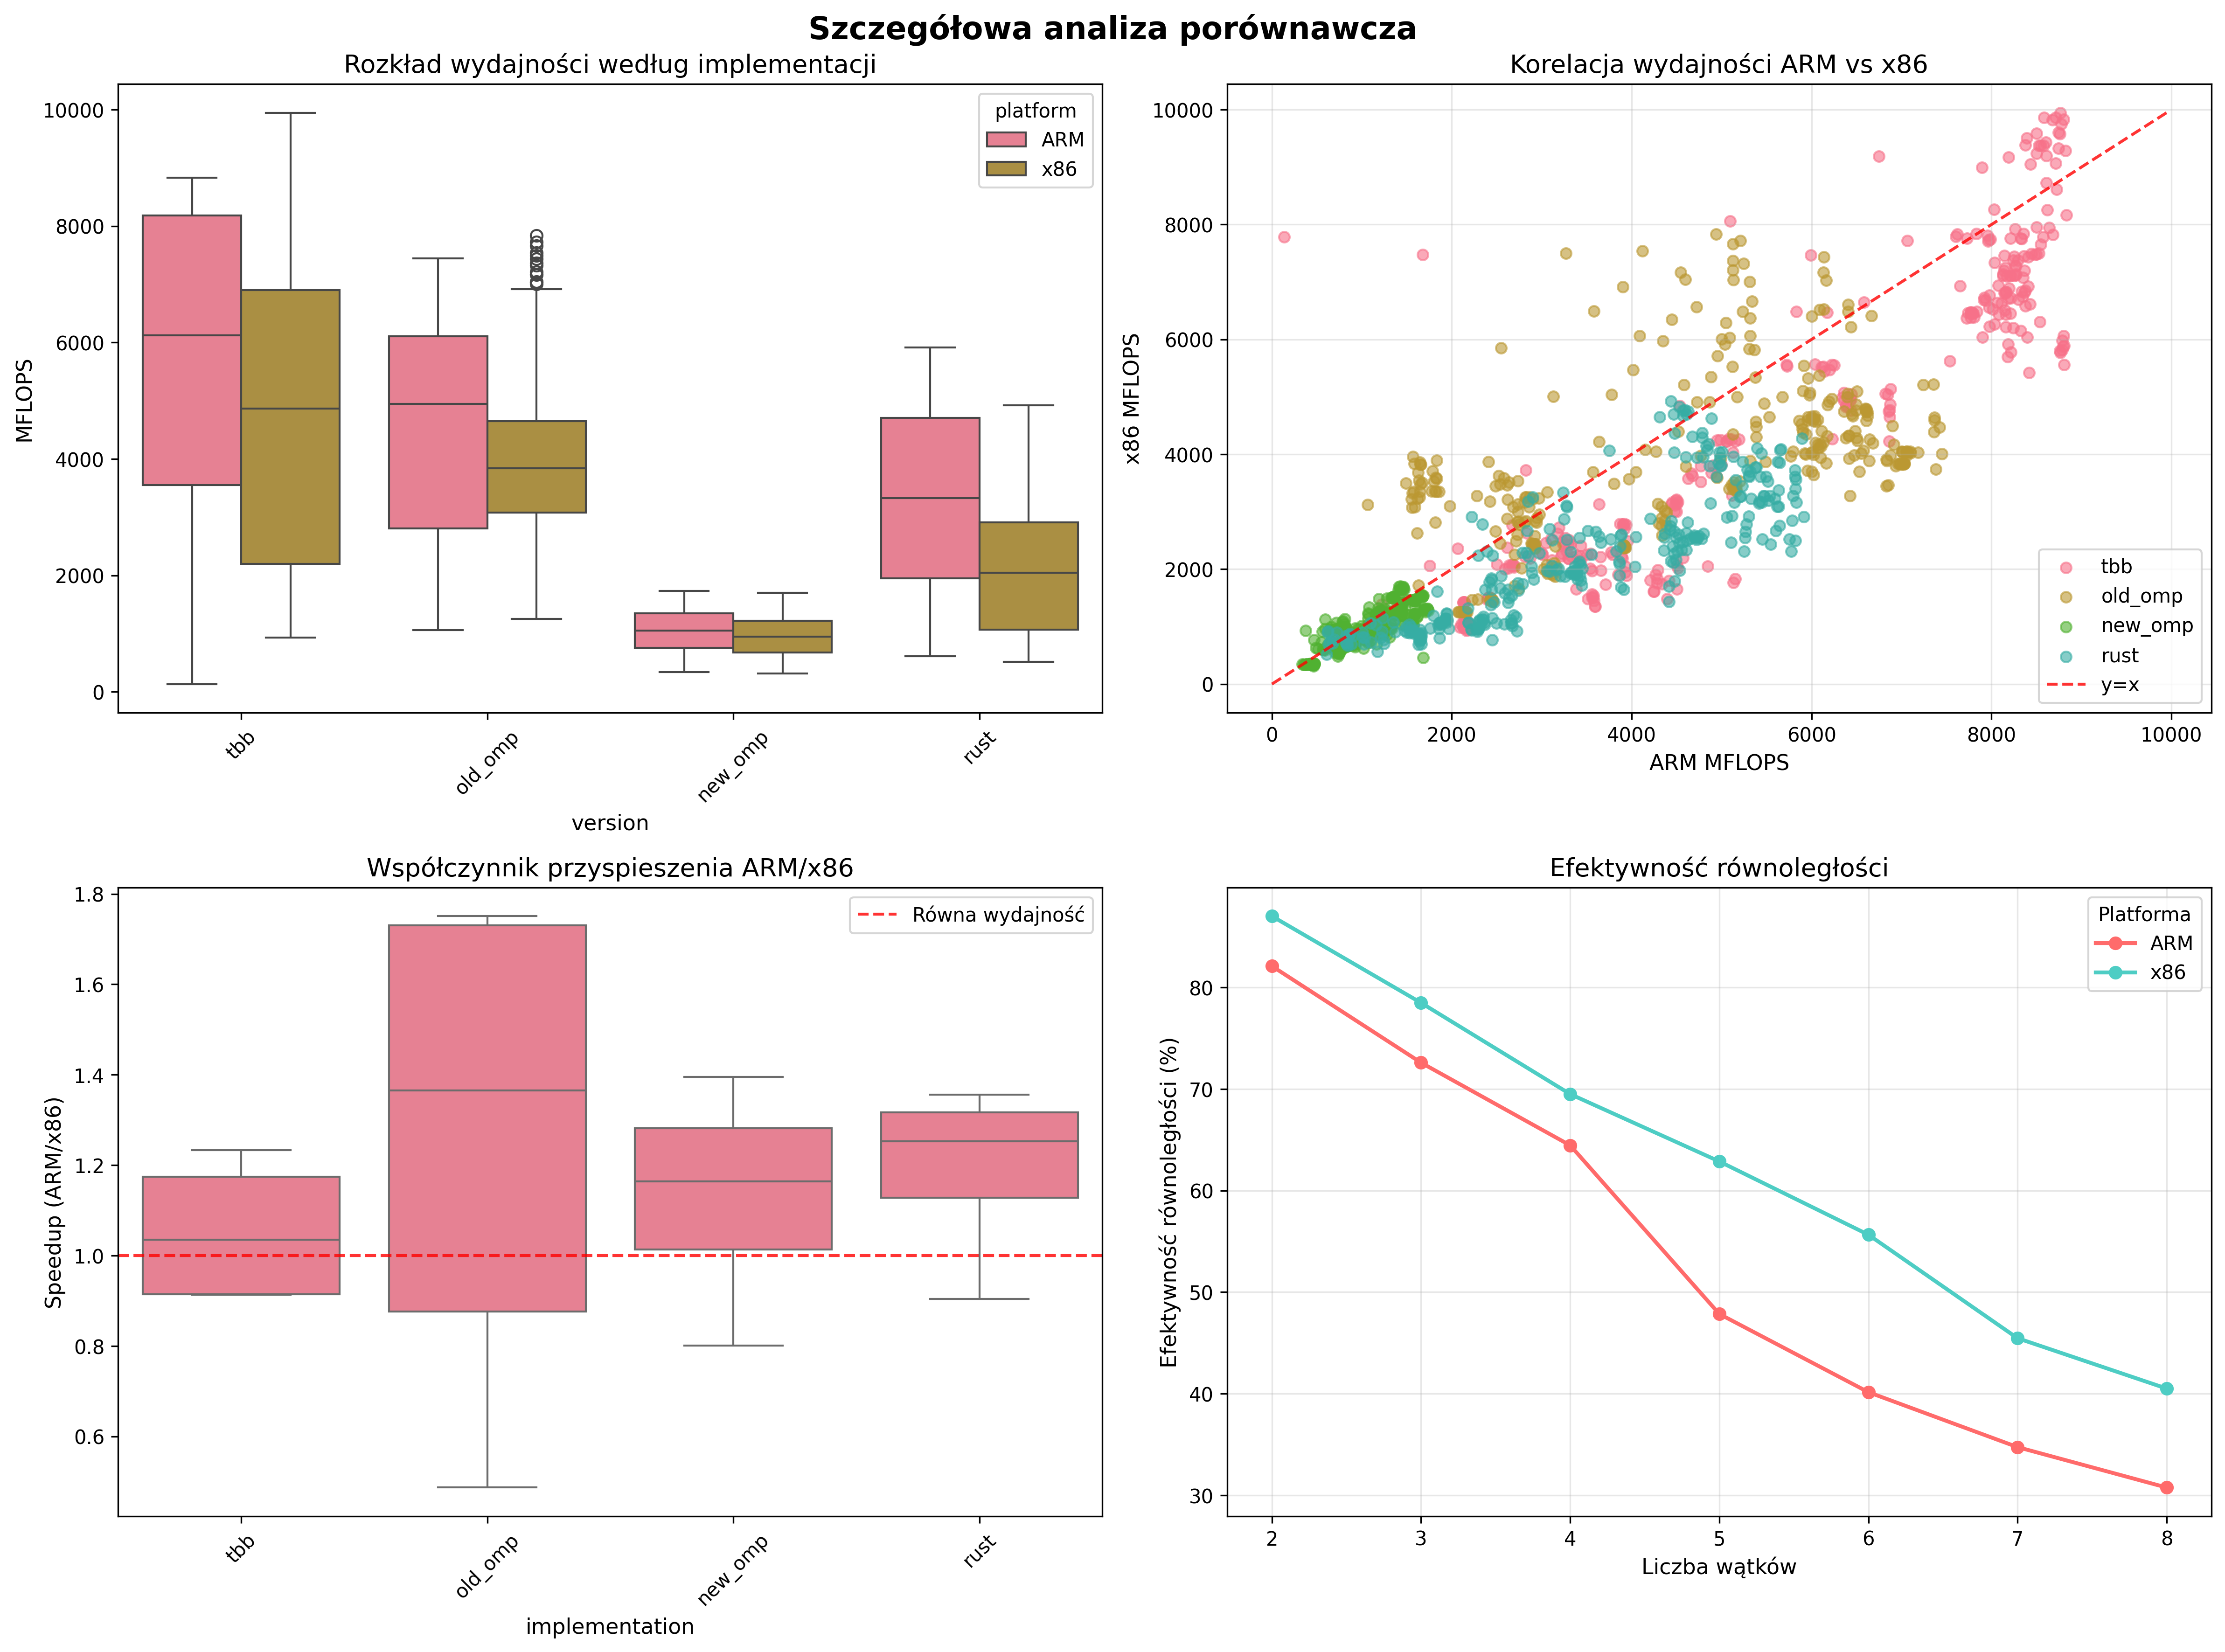
\includegraphics[width=\textwidth]{analiza/images/parallel/cg/compare/cg_szczegolowa_analiza_wydajnosci.png}
    \caption{Szczegółowa analiza wydajności benchmarku CG dla platform ARM64 i x86\_64}
    \label{cg_szczegolowa_analiza_wydajnosci}
\end{figure}
\subsubsection{Rozkład wydajności i korelacja}
Wykres pudełkowy obrazujące rozkład wydajności według implementacji pokazują większą zmienność wyników na platformie ARM, szczególnie dla tbb i old\_omp, co może świadczyć o bardziej dynamicznym zarządzaniu zasobami na poziomie systemowym (macOS). Mimo tej zmienności, wartości median są konsekwentnie wyższe dla ARM.

Wykres korelacyjny MFLOPS ARM a x86 ukazuje silną dodatnią korelację między wynikami na obu platformach, z większością punktów powyżej linii równej wydajności (y = x), co oznacza, że ARM zazwyczaj przewyższa x86 pod względem osiągów. W przypadku rust różnica jest szczególnie wyraźna.

\subsubsection{Efektywność równoległości}
Analiza efektywności równoległości (rozumianej jako stosunek osiągniętej wydajności do liczby wątków względem wydajności jednordzeniowej) wskazuje na wyraźnie wyższe wartości dla platformy x86 przy większej liczbie wątków. Podczas gdy ARM charakteryzuje się dobrą wydajnością bezwzględną, jego efektywność maleje szybciej wraz ze wzrostem liczby wątków, co może wynikać z wąskiego gardła na poziomie pamięci współdzielonej lub mniejszej liczby jednostek wykonawczych na wątek fizyczny.

\begin{figure}[H]
    \centering
    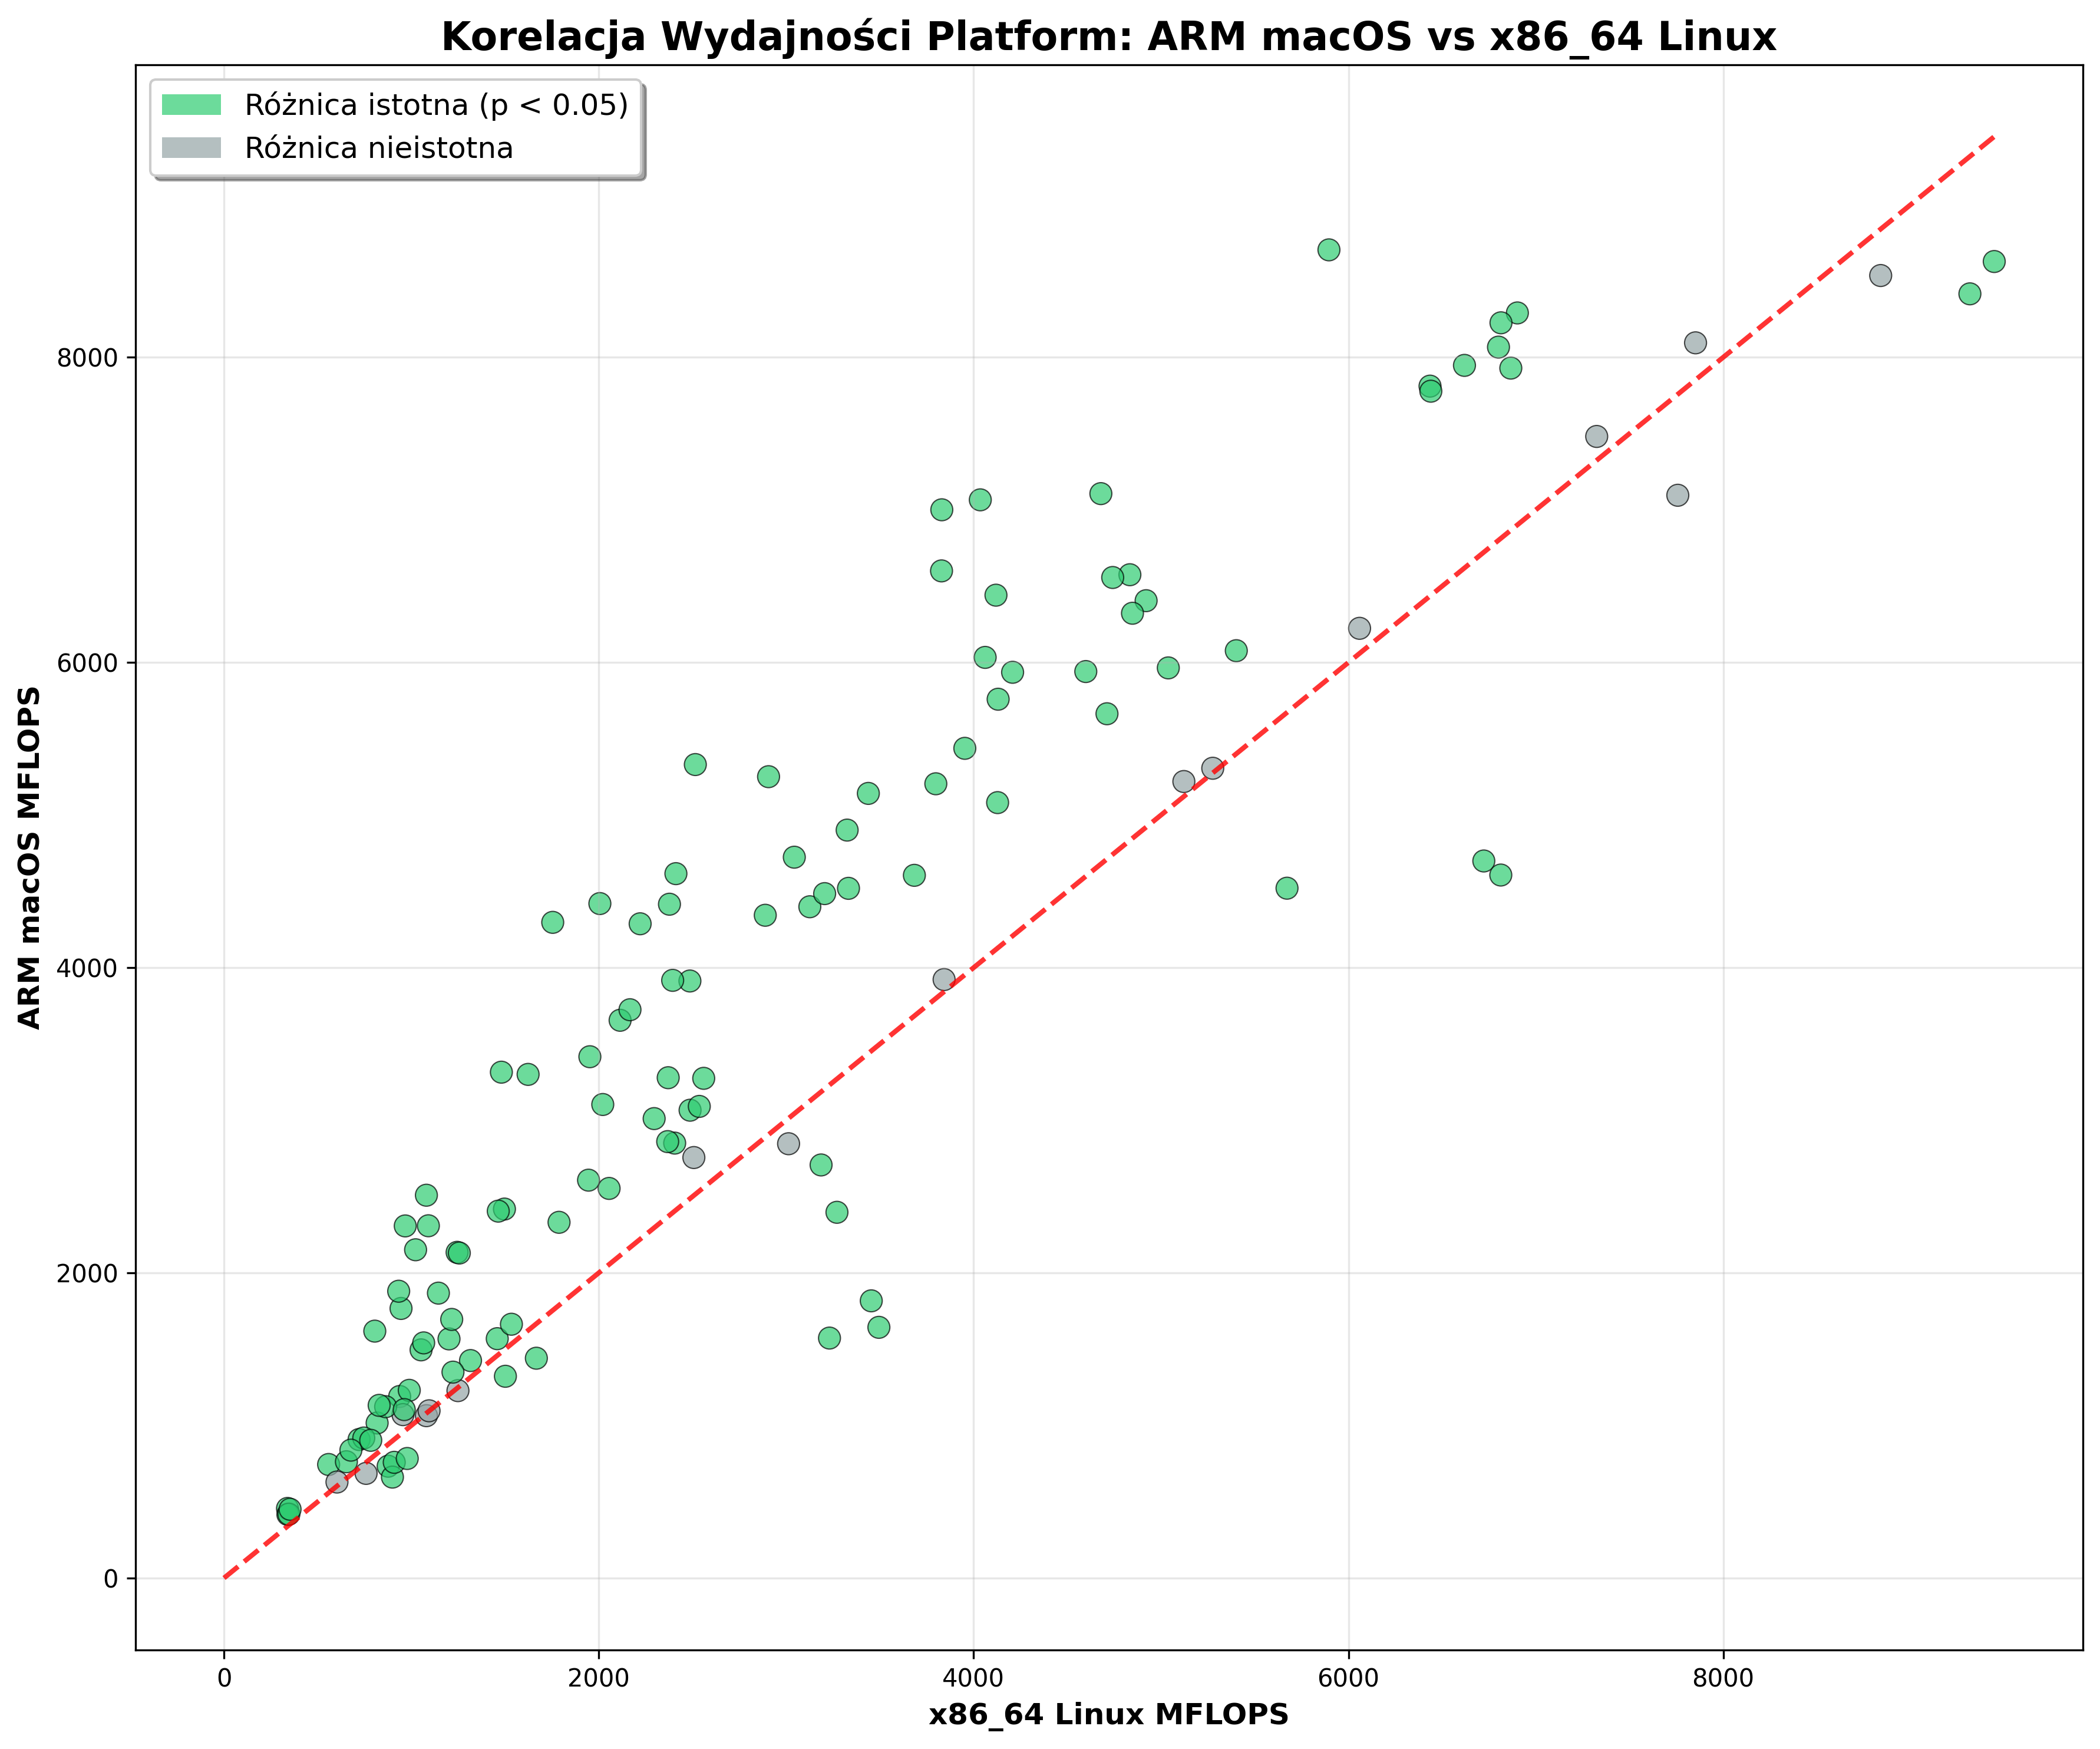
\includegraphics[width=\textwidth]{analiza/images/parallel/cg/compare/cg_analiza_istotnosci_statystycznej.png}
    \caption{Analiza istotności statystycznej benchmarku CG dla platform ARM64 i x86\_64}
    \label{cg_analiza_istotnosci_statystycznej}
\end{figure}
Na wykresie - rysunek \ref{cg_analiza_istotnosci_statystycznej} zaprezentowano korelację wydajności z uwzględnieniem istotności statystycznej (p < 0.05). Zdecydowana większość punktów (zielone oznaczenia) wskazuje na istotne różnice wydajności między platformami. Dla kilku przypadków (oznaczenia szare) różnica nie była statystycznie znacząca. Potwierdza to tezę, że platforma ARM macOS w większości przypadków przewyższa x86\_64 Linux, nie tylko nominalnie, ale również z punktu widzenia statystycznej wiarygodności wyników.